\documentclass[12pt]{book}
\usepackage[twoside,margin=1in,bindingoffset=0.5in]{geometry}
%\usepackage[round,authoryear]{natbib}
\usepackage{amssymb}
%\usepackage{tocbibind}
\usepackage{graphicx}


\usepackage{amsmath}
\usepackage{listings}
\usepackage{subcaption}
\usepackage[breaklinks = true, linktocpage, pagebackref,
colorlinks = true, hyperindex = true, hyperfigures] {hyperref}
\usepackage[grey]{quotchap}
\usepackage{pdfpages}

\hypersetup{
    colorlinks=false,
    pdfborder={0 0 0},
}

\usepackage{pdflscape}
\usepackage{afterpage}


\renewcommand{\bibname}{Reference List}

\begin{document}
\raggedbottom
%\openup .60em
% Set equal margins on book style
\setlength{\oddsidemargin}{53pt}
\setlength{\evensidemargin}{53pt}
\setlength{\marginparwidth}{57pt}
\setlength{\footskip}{30pt}
\openup 1em
%\includepdf[pages={1}]{titlePDF2}
\frontmatter
%\includepdf[pages={2}]{titlePDF2}
\makeatletter
\chapter{Abstract}

3D reconstruction algorithms generate 3D data from image or video data. The current focus of this research area is on iterative algorithms such as: feature matching/RANSAC, Iterative Closest Point, and other non-linear optimization strategies. These strategies tend to fail in scenes with few features or scenes which contain feature confusion. In 2D image registration research, feature matching is dominant but closed solution based Fourier registration techniques have been proven to outperform them with increased robustness to noise and low textured scenes. In this research, Fourier Volume Registration was explored in order to document the effects of 3D reconstruction and registration. Results are compared between Fourier Volume Registration, and several current techniques both quantitatively and qualitatively. Results show that the Fourier Volume Registration Technique often outperforms other methods in terms of minimizing registration error prior to optimization. Furthermore it is a closed solution which works well with parallel processing architectures. In conjunction, 3D data representations for 3D reconstruction data were also explored in order to improve storage and transmission of such data. Many current methods make use of Signed Distance Functions, volumetric occupancy grids or Octrees. Unlike previous work, lossy Octree compression is analysed. This direction paves the way for new storage and transmission rates of efficiency. A novel method called the Plane-Tree is proposed. The findings presented on both the Fourier Volume Registration method and the Plane-Tree indicate an improvement over existing methods and may lead to new research into the areas of Fourier registration and Hierarchical data representation research.


 % Abstract
\makeatletter
\chapter{Acknowledgements}

I would like to thank Dr. Ruben Gonzalez my supervisor, and myself for working so hard. I would also like to thank my wife Thao for her constant love and motivation.
\tableofcontents
\listoffigures
\listoftables
\mainmatter
%item : complete / required

%intro : 6/10\\
%lit-rev: 46/60\\
%meth : 28/60\\
%exps : 42/40\\
%conc : 2/10\\

%total: 173/180\\
%refs : 181/200\\

%re-factor plan
%Intro
%	3D reconstruction, aims & contributions, overview
%Background
%	Signal Registration
%	Depth Data Generation
%	Sensor Input Techniques
%	Data Representations	
%Pose Estimation
%	Fundamental Matrix
%	Feature Matching with RANSAC
%	ICP
%	SDF Optimization
%	3D Feature Matching
%	PCA
% 	Fourier Volume Registration
		%Recovery of Translation: overview, experiments
		%recovery of Y-Rotation: overview, experiments
		%A method for full 3D rotation recovery: overview, experiments
		%filtering techniques
		%speed improvements
%A 3D reconstruction method based on the Fourier Approach
	%pipeline,error metrics,reconstruction integration, advantages + disadvantages, experiments
%Data representations Revisited
	%octree
	%3D shadetree
	%plane-tree
	%octree subdivision
	%leaf node representation and computation
	%compression + decompression
	%experiments + analysis
%conclusion
%todo:
%research optimization methods
%work in the rgb-research into the methods parts
%put summary after the fft section
%do some slam techniques
%
%do some 3d representation stuff


\begin{savequote}[8cm]
  ``It is not knowledge, but the act of learning, not possession but the act of getting there, which grants the greatest enjoyment''
  \qauthor{Carl Friedrich Gauss}
\end{savequote}
\makeatletter
\chapter{Introduction}

\section{Introduction}



In recent years, there has been a resergence of research and applications within the areas of human computer interaction, these include: virtual reality, augmented reality and 3D reconstruction. This thesis concentrates on the area of 3D reconstruction. In this domain, image and video data is processed to collect 3D structural information. This information has many applications in virtual reality, engineering, architecture and business. Currently, there exist many methods which are capable of extracting 3D structural information from image and video data. Methods include: Feature Matching, Principal Components Analysis and Iterative Closest Point. These algorithms work well in simplistic environments where data noise and corruption is of no concern. Experiments reveal that using Fourier based registration can also recover 3D structural information by registering depth maps. This approach is shown to be robust to noise and object movement. It is capable of solving 1 axis of rotation as well as scale and translation. In cases where 3D rotation must be registered, a novel PCA/Fourier registration methods is proposed. Experiments show that in terms of registration accuracy, this method improves over ICP, feature matching and basic PCA, especially in the presense of noise. During experiments, it was discovered that 3D reconstruction data uses large amounts of storage. 3D data compression methods were also researched. During the PhD, a novel 3D compression method was developed. Results show this outperforms several state of the art methods in terms of low bit rate compression. This is useful for the fourier based registration methods as they are robust to data noise.

3D Reconstruction research requires the development, testing and analysis of functions which input video and image data and output 3D reconstructed environments. This area is very similar to Simultanious Localization and Mapping or SLAM. However, we have separated the areas as SLAM does not nececarily care about the full dense reconstruction of 3D data. It also has an added requirement of computing localization information. In 3D reconstruction, as long as pleasant, dense and useful 3D reconstructions are computed, localization does not matter.

3D reconstruction is imprortant in a wide variety of areas including business, engineerign and architecture, virtual reality and augmented reality. For example, an architect may want to record 3D structural data in order to study it later. An engineer may want to study the under area of a bridge in order to assess possible faults. Or a software engineer may want to create an augmented reality application where possible home buyers can take virtual tours through an existing property. The scpecifications and 3D structures of these areas may be recorded, in which case 3D models may be built by artists. This however, costs both time and money, furthermore there may be no existing blueprints for the structures, we may also want to provide virtual walking tours through a rainforest, this definately has no blueprint.

Using image and video capturing hardware coupled with 3D reconstruction software, we would be able to scan in an invornmemtn and generate a dense 3D model of it for use in egineering/architectural analysis as well as any kind of virtual reality application. Furthermore, autonomous navigation systems may also generate and use this information as they navigate through a previously unknown environment. Furthermore, with the recent progress made in 3D printing, we may come across a situation where 3D objects and environments may be scanned in using 3D recosntruction and copied via 3D printing.


Without such a system, artists, architects, engineers or scientists would have to build, draw or find some alternative means of generating the 3D data they require. This costs much time and money.

As in other areas of image processing, 3D reconstruction is dominated by feature matching and RANSAC techniques. This involves computing matches between 2D pixels across images, these matches are typically used with RANSAC to compute a camera relationship between the frames. 3D data is then projected and registered using the relationship. This approach is efficient but is not robust to data noise. Furthermore, without some outlier removal function to filter matches, this method fails as feature detection methods typically over-compute matches to the point that only around 30 - 50 percent of features are actually matched. This method also fails in cases where large baselines are used, affine distortion is too large, feature confusion occurs or other times when feature matching fails. Another popular method Iterative Closest Point can be used. This method is more robust to failure than feature matching, and can also be used with RANSAC. However, it fails when the search reaches a local minima in terms of matching error.

Despite the apparent flaws in these methods, they are still popular in both research and industry. In image processing however, alternatives exist. One in particular: Fourier based registration works well at computing 2D rotation, scale and translation. The benefits of this technique are that it is robust to noise and outliers as it takes into account the full signal (it uses the frequency domain to perform fast correlation of data). It is also a closed form sollution (its speed does not depend on the amount of features or on the data itself) and lends itself more easily to parallel processing, a paradime which is set to take over the next generation of software and hardware. Such techniques are frequently used in medical image processing. This raises the question of how well such a technique or related set of techniques would apply to the area of 3D reconstruction.

During the research conducted in quest of answering this question, it was found that the storage and thus manipulation of 3D data became a bottleneck for database and network based operations to do with 3D reconstructed data. To alleviate this issue, compression techniques were also analysed. A set of novel techniques for compression and storage of 3D data are also proposed in this work.  

\section{Research Aims \& Contributions}

The primary aim of this research is to improve the accuracy, noise robustness, speed and storage, quantitative quality and perceptual quality of 3D models. To this end, fourier based registration schemes were investigated as well as compression systems. This motivated the research question, ``Can Fourier based registration techniques improve accuracy and noise robustness in 3D reconstruction applications?'' and ``Can hierarchical techniques improve compression, storage and processing of 3D reconstruction data?'' 

The quest to answer these questions has led to new 3D registration techniques \cite{Lincoln13Interpolating} which outperform ICP and feature matching approaches in terms of noise robustness and accuracy. A novel compression scheme was also developed which was shown to be capable of outperformign existing schemes, this method may be applied to 3D reconstruction storage and retrieval applications and research.

\section{Overview}

Chapter two presents a survey of techniques which may be used for 3D reconstruction. Following this, chapter three introduces some proposed techniques. These are used to answer the research questions and accomplish the primary aim of this project. The fourth chapter details the experiments performed, and presents both quantitative and qualitative results. The fifth chapter contains an analysis of these results and presents findings and discusses results. Finally, the sixth chapter concludes the thesis and discusses the results in terms of the primary aim and research question. 


 % The Introductory Chapter
\begin{savequote}[8cm]
  ``He who controls the past controls the future.''
  \qauthor{George Orwell, 1984}
\end{savequote}
\makeatletter
\chapter{Literature Review}

\section{Introduction}

In this section we review some of the crucial areas and techniques involved in both Simultaneous Localization and Mapping (SLAM) and registration. First, some important registration techniques are covered including both feature matching and phase correlation. Then, depth data generation is covered. These techniques assist with the generation of dense 3D data used for 3D reconstruction. Another important area: Pose estimation is also We begin with an overal tutorial on 3D-SLAM before covering registration. Next, 3D reconstruction data-representations and compression schemes are covered. 


%registration techniques [basics]
\section{Signal Registration}
\subsection{feature matching}


Harris and Stephens \cite{Harris88Combined} invented the Harris corner detector. This detector uses a variable sized window around each pixel, in which a Harris matrix is formed from the x, y and xy gradients. The Harris response is calculated using the determinant and trace of this matrix. Several years later, Smith and Brady \cite{Smith97Susan, Smith92New} presented a feature detector called SUSAN. SUSAN is an alternative to second order methods for corner detection and uses a non-linear filter to find corners and edges. SUSAN also naturally provides feature vectors. It works by surrounding each pixel with a circular non-linear kernel for filtering. The kernel's response is defined as the area within the kernel having the same or similar value to the nucleus (center of the kernel). Walker et al \cite{Walker98Locating} used a classification (machine learning) method to find salient places in images.\\


Trajkovic \& Hedley \cite{Trajkovic98Fast} presented a fast yet simple corner detection algorithm. This method computes the minimum intensity changes in all directions. It is fast as it only uses a 3x3 window for the corner response function. This method is compared to the Harris and Susan corner detectors. It is faster than both these methods whilst also being more robust than the Susan corner detector. Harris is the more accurate corner detector in terms of repeatability and detection.\\


Lowe's \cite{Lowe04Distinctive,Lowe99Object} method, SIFT (Scale Invariant Feature Transform) is a popular method for feature extraction and description. The method computes features at different scales using an image pyramid and difference of Gaussian to approximate the Laplacian of Gaussian. Features are represented using a vector of weighted gradients surrounding the feature. The descriptor is invariant to scale because of each descriptor is found at some scale within the multi-resolution pyramid. SIFT is rotationally invariant if the window is chosen so that its angle of origin is based on the angles surrounding the feature. It is invariant to luminance because of the use of gradients, and since features are described by the surrounding window of the feature, they are invariant to translation. This method is said to be robust to 3D viewing transforms and affine transforms. SIFT was also developed to run faster on GPUs \cite{Wu07Siftgpu}. \\


Tuytelaars \& Van Gool \cite{Tuytelaars00Wide} developed a method for detecting and describing affine invariant regions. These regions are computed directly from intensity values in the image using rays extending from the center of regions. Feature vectors made up from statistical moments within the regions, then nearest neighbour matching is used to match features. Boykov \& Jolly \cite{Boykov01Interactive} presented a method for region based feature extraction. This method uses graph cuts to find which regions are adequate features. This method requires some soft constraints performed by humans so is not good for automatic detection of features, also because features are not very localized their size and shape is not viewpoint invariant.\\


Itti \& Koch \cite{Itti01Computational} presented a biologically inspired bottom up image saliency detector. Schaffalizky and Zisserman \cite{Schaffalitzky01Viewpoint} developed a texture based region descriptor. It is invariant to photometric and affine transformations. It is also insensitive to the shape of the region and can be used to compute epipolar geometry. This method makes use of the second order matrix. Mikolajczyk and Schmid \cite{Mikolajczyk01Indexing} presented a new feature point detector and descriptor. Their detector is based on multi-scale Harris in which they then use to filter the points by the value of the surrounding Laplace. For feature description they use Gaussian derivatives. \\


Carson et al \cite{Carson02Blobworld} developed a method for image feature classification and matching called Blobworld. This method segments an image before using region vectors for image querying and feature matching. This technique begins by defining a pixel neighbourhood size, it then groups pixels together based on the texture and colour data within one of these neighbourhoods. Finally, vectors describing colour and texture are formed for each region and these are used in image queries. Sebe et al \cite{Sebe03Evaluation} compared local based feature detectors, their proposed method uses a wavelet saliency extractor, making use of textures and colour in order to obtain invariance in its descriptor. \\


Kadir et al \cite{Kadir04Affine} developed a saliency based method for feature detection. This method is scale, viewpoint and perturbation invariant. Carbonetto et al. \cite{Carbonetto04Statistical} presented a method which segments images, labelling them with feature vectors made up of descriptive words. Image region mapping can be performed by statistically comparing feature description vectors. Matas et al \cite{Matas04Robust} developed a new feature detection and description method called MSER. This algorithm uses small regions as features instead of a single point and surrounding window. These regions are calculated by taking the foreground blobs of an image at every possible binary threshold. MSER detection and representation is invariant to scale (3.5 x), illumination, out-of-plane rotation, occlusion, locally anisotropic scale change and 3D translation of viewpoint. \\

Mikolajczyk and Schmid \cite{Mikolajczyk05Performance} performed an evaluation of local feature descriptors. They performed a comparison between shape-context, PCA-SIFT, differential invariants, spin images, SIFT, complex filters, moment invariants and cross correlation. They also present their method called GLOH, which is an extension of the SIFT descriptor. Results indicate that GLOH and SIFT perform the best. Rosten \& Drummond \cite{Rosten06Machine,Rosten05Fusing} aimed to improve the speed of feature detection over SIFT and SUSAN. They developed a technique called FAST (Features from Accelerated Segment Test), this method tests the difference between the center pixel and its surrounding pixels within the surrounding circle. They also improved this approach by first extracting FAST corners, then classifying these corners using a decision tree to extract better feature points, whilst retaining speed. Both FAST and FAST-ML (FAST with Machine Learning) methods are shown to be faster than SIFT and SUSAN whilst FAST-ML is also shown to be more reliable at classifying the same features from different viewpoints. Another method, ORB \cite{Rublee11Orb} is based on FAST and BRIEF \cite{Calonder10Brief}. ORB detects features similarly to FAST and computes rotation and feature descriptors similarly to BRIEF. It is shown to be robust to viewpoint changes and is faster than SIFT and SURF.  \\ 


Bay et al \cite{Bay06Surf,Bay08Speeded} improved the speed and accuracy of feature matching compared with SIFT using their method named SURF (Speeded Up Robust Features). In SURF, a Hessian matrix is used for the detection of features whilst Haar wavelet components are used as descriptors. A non rotation invariant version was also analysed and proved to be faster. This version is suitable if rotation invariance is not required for a particular application. Lepetit and Fua \cite{Lepetit06Keypoint} turn the wide stereo baseline matching problem into a classification problem. This method is stated to be robust, accurate and real-time. The training phase attempts to classify repeatable corners. The training set is built from many different rasterizations (which affect illumination) of only a few images. Key-points are extracted at multiple octaves and scales at the surrounding image patch. The authors report randomized trees as being the optimal machine learning method for their technique. \\


Cabani \& MacLean \cite{Cabani07Implementation} presented a feature detector based on the Harris point operator. This method detects affine invariant features using the speed of an FPGA. It can process images of 640 x 480 at up to 30 frames per second. This technique is compared to C and Matlab versions of the same process. Finally, Tuytelaars and Mikolajczyk \cite{Tuytelaars08Local} presented a survey on feature detectors. They provided a detailed introduction to the subject and categorize different feature types and techniques. \\

\subsection{phase correlation}

Phase correlation is a technique used in digital signal processing to register two sgianls, images or 3D volumes with translation differences. It is robust to noise and view-point changes. Techniques in phase correlation can be used to find additional parameters (such as rotation, scale and sheer). Fourier methods such as phase correlation can therefore be used to compute camera pose without the need for least squares approximations or the use of ICP (which cannot recover scaling parameters). \\ 

Digital signal processing is the scientific area concerned with the acquisition, filtering, processing and understanding of digital signals using computer technology. Digital signals are simply an array of numbers, digital images are 2D signals. One of the fundamental ideas behind this research area is that digital signals can be processed using a set of common techniques regardless of where or how they were generated. There are two fundamental techniques used in digital signal processing. One is the use of correlation and convolution, the other is the use of alternative representations (eg. the Fourier transform). For in depth details of these concepts read \cite{Smith97Scientist}. Convolution is the process by which one signal is used to filter another whilst correlation is used to measure the similarity between one signal and another at different phases. The Fourier transform is used to transform signals (in the time domain) into the frequency domain. The frequency domain represents the original signal using a set of sine and cosine waves at different frequencies. The time domain is the name given to the original domain of the signal. This transform is performed by correlating the signal with sine and cosine waves at varying frequencies. A transform called the inverse Fourier transform can be used to transform a signal from the frequency domain back to the time domain. \\

The inputs and outputs of the Fourier transform are digital signals made up of complex numbers. Most of the time, the input signal is not complex (as in the case of a photographed scene). In this case imaginary value scalars of zero are augmented to the signal to make it complex. The frequency domain can be visualized easily using the polar representation of these complex numbered signals. The polar representation represents the signal using the magnitude and phase of sine waves at different frequencies and directions (in the case of 2D). This can be visualized in figure \ref{fig:PCSecA}, here the magnitude represents the height of the sine waves, the phase represents the translation from the origin in which these waves occur and the 2D position within the image represents the direction the waves travel in 2D. The most useful aspect of the Fourier transform is that when signals are represented in the frequency domain, their point-wise multiplication is equivalent to convolution in the time domain. This is important because convolution is a computationally intensive process, especially in image processing where there is a lot of data to process. \\

\begin{figure*}[t!] 
        \centering
        \begin{subfigure}[b]{2.0in}
                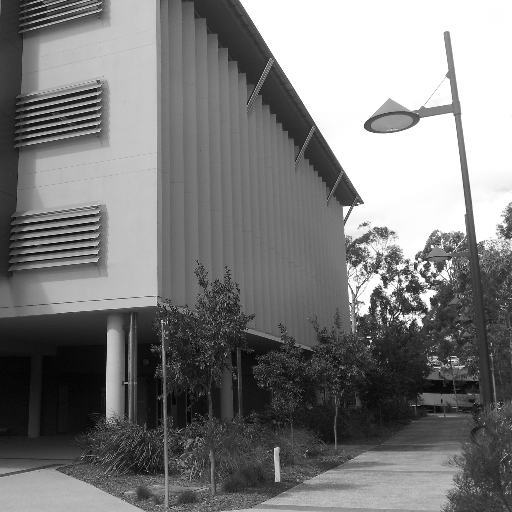
\includegraphics[width=1.5in]{images/pc/original}
                \caption{original}
                \label{fig:PCSecOrig1}
        \end{subfigure}%
        \begin{subfigure}[b]{2.0in}
                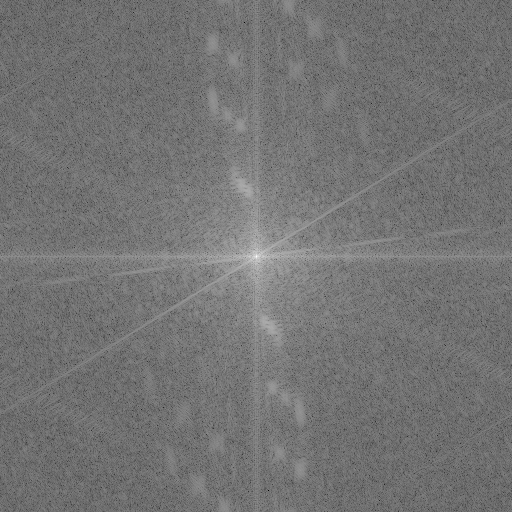
\includegraphics[width=1.5in]{images/pc/magnitude}
                \caption{magnitude}
                \label{fig:PCSecMag}
        \end{subfigure}%
                \begin{subfigure}[b]{2.0in}
                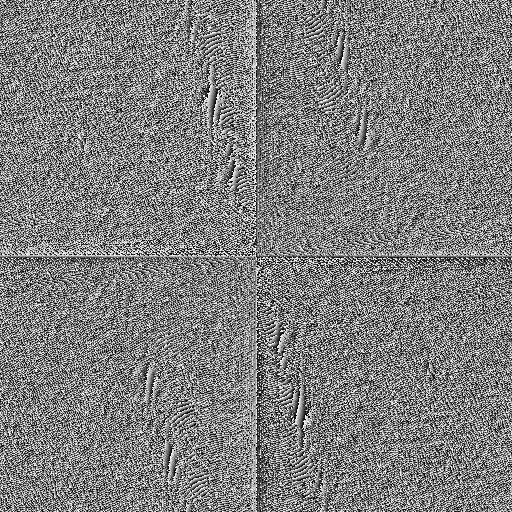
\includegraphics[width=1.5in]{images/pc/phase}
                \caption{phase}
                \label{fig:PCSecPhase}
        \end{subfigure}%        
       \caption{The polar representation of the Discrete Fourier transform on an input image.}\label{fig:PCSecA}
\end{figure*}

Phase correlation is the process of using the frequency domain representation to perform image registration using correlation. In image processing, this allows us to find the translation parameters between two images (does not work if rotation or scaling is introduced) efficiently. This can be performed by flipping one image before transforming both into the frequency domain. Since point-wise multiplication in the frequency domain causes convolution in the time domain, flipping one image causes correlation in the frequency domain which is what is required. Once this correlation is performed, the inverse Fourier transform is performed, the output image contains a peak which is used to compute the translation different between the two images. This can be visualized in figure \ref{fig:PCSecCC}. Here, the original image is translated from figure \ref{fig:PCSecORY} to figure \ref{fig:PCSectrans} and the two are phase correlated producing the peak in figure \ref{fig:PCSecCCPC} which represents the translation between the two. \\


\begin{figure*}[t!] 
        \centering
        \begin{subfigure}[b]{2.0in}
                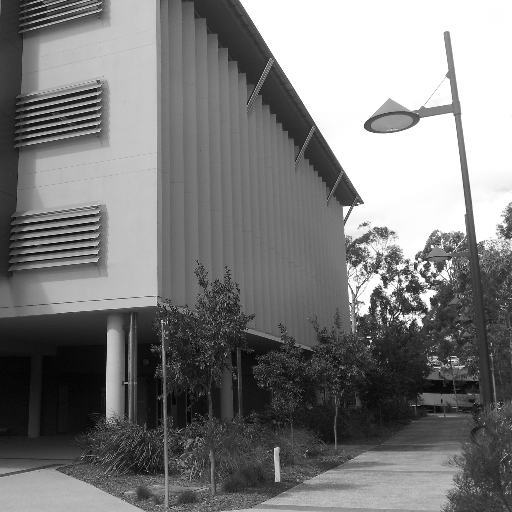
\includegraphics[width=1.5in]{images/pc/original}
                \caption{original}
                \label{fig:PCSecORY}
        \end{subfigure}%
        \begin{subfigure}[b]{2.0in}
                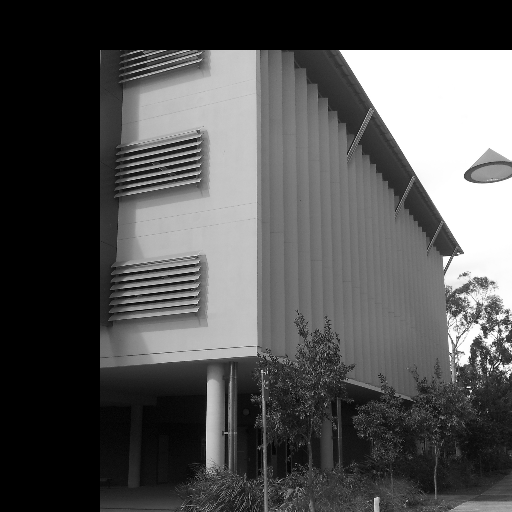
\includegraphics[width=1.5in]{images/pc/translated}
                \caption{(a) translated}
                \label{fig:PCSectrans}
        \end{subfigure}%
                \begin{subfigure}[b]{2.0in}
                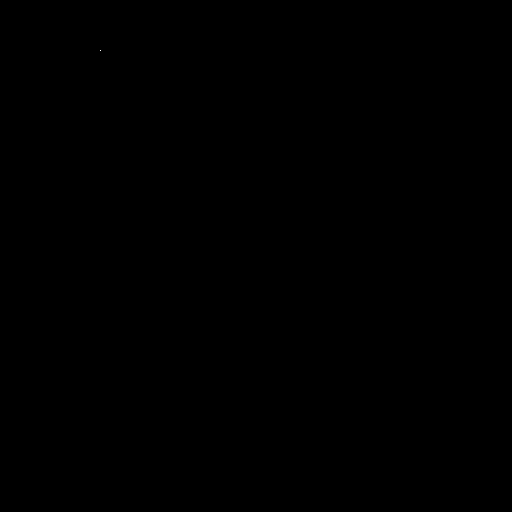
\includegraphics[width=1.5in]{images/pc/phasecorrelation1}
                \caption{correlation}
                \label{fig:PCSecCCPC}
        \end{subfigure}%        
       \caption{Phase correlation used to align two images seperated by a translation.}\label{fig:PCSecCC}
\end{figure*}

The other parameters we wish to estimate for registration are the scale and rotation parameters, however another type of transform is introduced first. This image transform is called the log-polar transform. This transform re-arranges the pixels from euclidean 2D space $[x,y]$ to the polar space $[log(sqrt(x^2+y^2)),atan(y/x)]$ where rotation about the center is turned into y-axis translation and scaling about the center is turned into x-axis translation. This representation changes any rotation and scaling performed on the image into translation. Translation parameters can be easily found using phase correlation. This process can be visualized with the help of figure \ref{fig:PCSecB}. The problem is, the rotation and scaling has to be about the center of the image, which is an issue if the images contain a translation added to them. Luckily, in the magnitude of the polar representation of the frequency domain the effects of translation are not present. On top of this, any sort of rotation or scaling (whether translation is present or not) occurs about the center of the image. \\

\begin{figure*}[t!] 
        \centering
        \begin{subfigure}[b]{1.5in}
                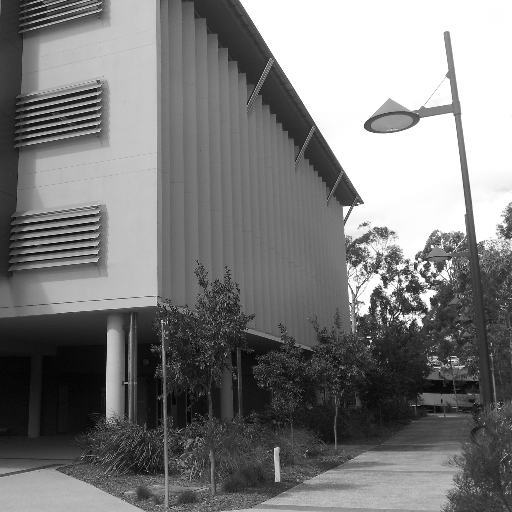
\includegraphics[width=1.4in]{images/pc/original}
                \caption{original}
                \label{fig:PCSecOrig2}
        \end{subfigure}%
        \begin{subfigure}[b]{1.5in}
                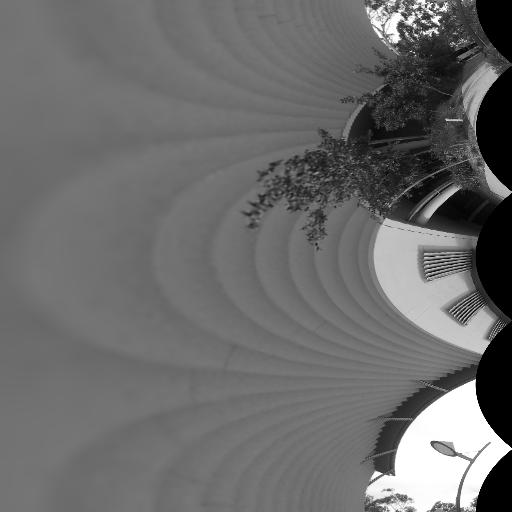
\includegraphics[width=1.4in]{images/pc/logpolar}
                \caption{log-polar of (a)}
                \label{fig:PCSecLP}
        \end{subfigure}%
         \begin{subfigure}[b]{1.5in}
                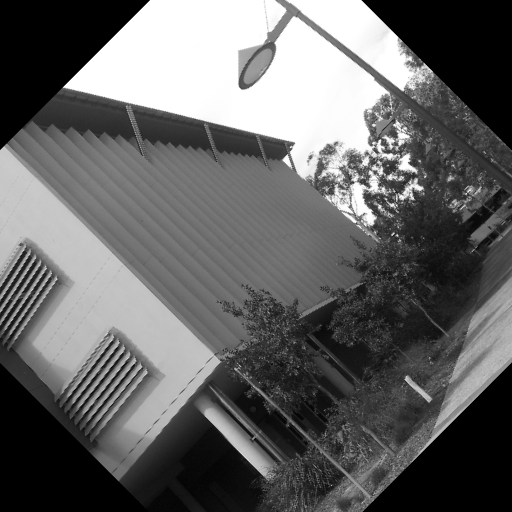
\includegraphics[width=1.4in]{images/pc/rotation}
                \caption{rotation by -45 ${}^{\circ}$}
                \label{fig:PCSecRot}
        \end{subfigure}%
        \begin{subfigure}[b]{1.5in}
                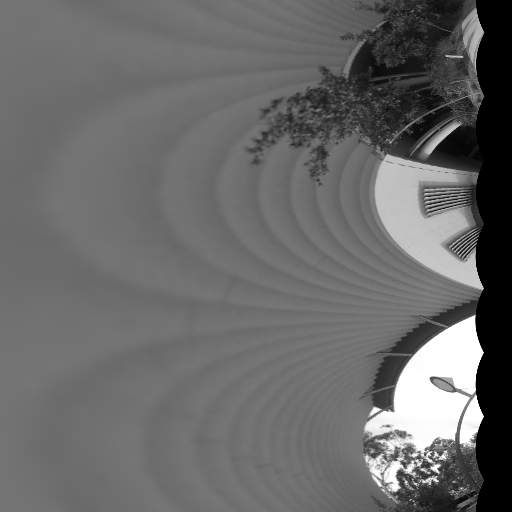
\includegraphics[width=1.4in]{images/pc/logpolarRotation}
                \caption{log-polar of (b)}
                \label{fig:PCSecLPR}
        \end{subfigure}
         \begin{subfigure}[b]{1.5in}
                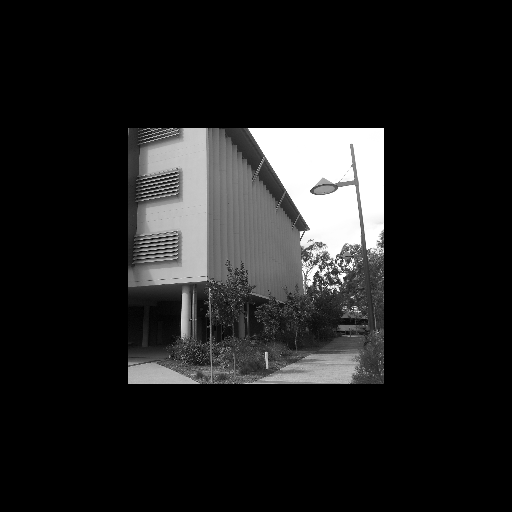
\includegraphics[width=1.4in]{images/pc/scaled}
                \caption{scaled by 0.5}
                \label{fig:PCSecOrig2}
        \end{subfigure}%
        \begin{subfigure}[b]{1.5in}
                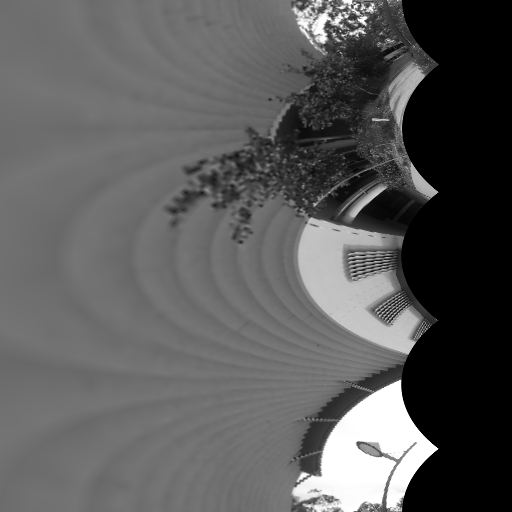
\includegraphics[width=1.4in]{images/pc/logpolarScale}
                \caption{log-polar of (c)}
                \label{fig:PCSecLP}
        \end{subfigure}%
                \begin{subfigure}[b]{1.5in}
                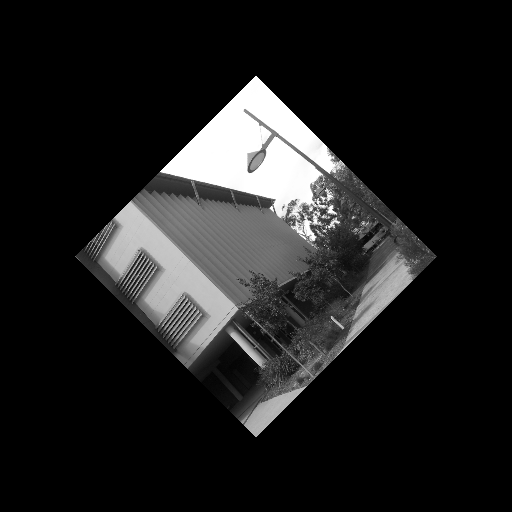
\includegraphics[width=1.4in]{images/pc/rotationscale}
                \caption{rotation + scaling}
                \label{fig:PCSecRot}
        \end{subfigure}%
        \begin{subfigure}[b]{1.5in}
                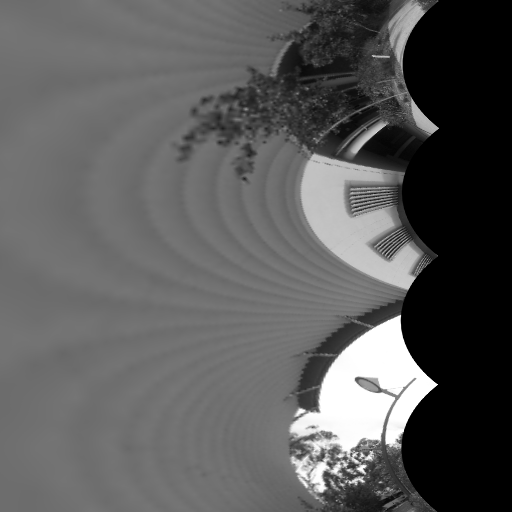
\includegraphics[width=1.4in]{images/pc/logpolarRotationScale}
                \caption{log-polar of (d)}
                \label{fig:PCSecLPR}
        \end{subfigure}%        
       \caption{The effects of the log polar transform.}\label{fig:PCSecB}
\end{figure*}

This allows the phase correlation method to recover the translation, scaling and rotational information between two images. First, the magnitude of the polar representation of both the images is computed. Then both magnitudes are log-polar transformed and phase correlated. This finds the scaling and rotational parameters. Both of the original images have their rotation and scaling reversed, then both images are phase correlated to undo the effects of translation, which is the final parameter to compute. In this way, translation, scaling and rotational parameters can be computed directly without the need for feature matching and least-squares estimation of the transformation matrix. \\


%depth data generation and pose estimation
\section{Depth Data Generation} \label{DepthDataGenSection}

In 3D reconstruction, dense depth data is very important, without it there is no dense 3D reconstruction, only sparse mapping. This section introduces some techniques and research on different methods (both hardware and software) of depth data generation. In the first section the use of sensors which are capable of generating depth data is introduced. Next, methods using stereo camera pairs are discussed. Finally, monocular techniques are discussed. \\


\subsection{Sensors}

In 3D reconstruction, it is often ideal to use specialized sensors which capture reliable and dense depth data on a per pixel basis. One such camera is the RGB-D (Red, Green, Blue \& Depth) camera. These sensors are becoming more accurate and less expensive and are now found in mobile technologies. \\

Research by Zhang et al \cite{Zhang12Microsoft} used an RGB-D camera to generate smooth, continuously updating dense 3D reconstructions using only depth data. Here, using the data, 6 degrees of freedom were tracked. This techniques uses depth information only, and as such it works in the absence of visual light (it works in the dark) unlike passive camera approaches \cite{Klein07Parallel, Newcombe10Live,Stuhmer10Real} and techniques which use color data along with depth data \cite{Henry10Rgb}. \\

The Kinect is one such rgb-d camera. It uses a structured light based depth sensor along with an application specific integrated circuit to generate an 11-bit $640\times 480$ depth map at 30 times per second (real-time). \\

There is no doubt that these sensors are the easiest way to compute ready dense depth data for 3D reconstruction, but there are several drawbacks. Depth images contain holes. This is caused by a lack of structured light on a captured surface. Some materials simply do not reflect infra-red light (surfaces at steep angles or very thin objects). Also, when moving fast, the device easily experiences motion blur which leads to missing and incorrect data. \\

Some 3D reconstruction techniques use the approach of dense mapping and tracking via depth sensors and lasers. These approaches usually compute feature matches to align the frames or some sort of error minimization function.


\subsection{Stereo Cameras}

\label{StereoMethodsSection}

Stereo camera set-ups employ two cameras capturing a singular scene. Using a variety of techniques, depth data is computed from the stereo pair by measuring parallax. Stereo cameras may be calibrated or un-calibrated. Un-Calibrated stereo pairs require calibration using the Fundamental or Essential matrix, whilst pre-calibrated cameras require no further action before parallax may be computed. Using a variety of pose estimation techniques, the dense depth data may be integrated forming a 3D reconstruction. \\

In this section, some important techniques proposed within the area of depth data generation via stereo algorithms. Readers wanting to research techniques prior to 2005 are encourages to seed a survey by Scharstein and Szeliski \cite{Scharstein02Taxonomy}. \\


Sun et al \cite{Sun05Symmetric} presented an occlusion handling stereo matching algorithm. Their method incorporates a visibility constraint into the energy function for the belief propagation global optimisation method. Klaus et al \cite{Klaus06Segment} devised a stereo correspondence algorithm which uses colour segmentation combined with a self adapting matching score which minimizes the number of reliable occurrences. This method also uses belief propagation to assign a single disparity to each segmented region. Hirschmuller \cite{Hirschmuller05Accurate} proposed a semi-global matching method based on mutual information and approximation of a global smoothness constraint. \\

Yoon \cite{Yoon06Adaptive} presented work on a local method for computing disparity. In this method, the window is weighted based on geometric proximity and colour similarity. Darabiha et al \cite{Darabiha06Reconfigurable} presented an FPGA based local window stereo algorithm. This method obtains sub-pixel accuracy for 256$\times$360 images at 30 frames per second. Their window matching method uses correlation. Klaus et al. \cite{Klaus06Segment} devised a stereo method which segments the image before fitting regions with disparities. This fitting is based on interpolating depth values along each region. A self adapting matching score for segments is also used to maximize correspondences. Belief propagation is then used to optimize depth among the regions. \\


Yang et al \cite{Yang07Spatial} came up with a method which uses super pixel resolution to improve disparity images. First a depth map is computed at a lower resolution, it is then up-sampled to the same resolution as the corresponding colour image. The depth map is then used as a hypothesis to compute a cost volume, which is bilateral filtered. Then, a winner take all and a sub pixel estimation procedure are performed to estimate the full resolution depth map. This method is shown to improve sub-pixel resolution by up to 100 times compared to previous methods.\\


Sarkis et al \cite{Sarkis07Fast} improved the efficiency of the graph cut global optimisation based disparity algorithm whilst maintaining similar accuracy. Their method involves splitting the global space up using a quad-tree. Each space has an adapted energy function which is minimized using the graph cuts algorithm. Results show this method improves efficiency by up to 3 times over similar works. Wang and Zheng \cite{Wang08Region} came up with an inter-regional cooperative optimization based stereo correspondence technique. This method uses a local adaptive window based approach to compute an initial depth map. The original image is also segmented using a colour based mean shift technique. The segmented image and the initial depth map are then input into a region based optimization method.  \\


Yang et al. \cite{Yang08Near} attempted to solve the problem of stereo mapping for texture-less image regions. These regions are known to be difficult because there is less texture to correlate with. They use colour segmentation and plane-fitting with loopy belief propagation for error correction. Wang and Zheng \cite{Wang08Region} used a stereo method which uses image regions, plane fitting and segmentation as well as a novel region stereo optimization method. Ernst and Hirshmuller \cite{Ernst08Mutual} presented a GPU implementation of the semi-global matching technique (scan-line optimization) for stereo correspondence. Bleyer et al \cite{Bleyer09Stereo} devised a method which extracts disparities and alpha matting information at the same time. Alpha matting is used to generate artificial views for viewpoint effects. This method divides the image up into segments and computes the depth and alpha value for each of these segments. \\


Bleyer and Gelautz \cite{Bleyer09Temporally} presented a method for generating stereo disparity information from an un-calibrated stereo video. First, the video is segmented into scenes. Next, the two camera shots are calibrated before dynamic programming is used to optimize the disparity calculation. Then the disparity estimates are smoothed temporally in order to achieve robustness to disparity flickering. Hirschmuller and Sharstein \cite{Hirschmuller09Evaluation} presented a survey on stereo depth mapping with respect to radiometric differences. They investigated different metrics used in local matching methods as well as their relationship with radiometric variations. Also investigated were the effects of different filters: Laplacian of Gaussian (LOG), bilateral background subtraction, rank, SoftRank, census and ordinal. \\


In his masters thesis, Olofsson \cite{Olofsson10Modern} presented a survey and evaluation of various global and local stereo vision methods. He also presented a novel and efficient local method. This technique is shown to achieve state of the art results with some datasets. Bleyer et al \cite{Bleyer10Surface} introduced a method which models stereo images using smooth surfaces. This technique is based on the assumption that the entire scene is composed of a few smooth surfaces, and each pixel is a part of a surface. Colour segmentation is used to estimate different surfaces. Bleyer et al \cite{Bleyer11Patchmatch} presented a variation on the Patchmatch algorithm (PMA). PMA is a global optimisation method which models each pixel as a plane in 3D space. Each pixel is set to a random value within a larger region, as long as there is at least one close guess for the planes of one of the pixels, this information can be propagated. The default PMA performs spatial propagation, and uses adaptive support weighting to improve correspondence around the border. The method by Bleyer et al introduced view and temporal propagation to the original PMA. \\


Bleyer et al \cite{Bleyer11Object} later presented a joint stereo matching and segmentation algorithm. This method models segmented regions as objects having colour and a disparity distribution, they also use a novel 3D connectivity property for each object region. Lu et al \cite{Lu11Revisit} presented a method for increasing depth map quality given a colour original of the same scene at higher resolution. This allows disparity maps to be computed quickly by computing a lower resolution depth map before scaling-back the resolution. This method makes use of markov random fields and is unique in applying the technique to super pixel resolution in terms of depth mapping. This method is also uses state of the art disparity computation algorithms and so improves efficiency whilst retaining accuracy. \\ 


De-Maeztu et al \cite{De11Linear} presented a novel cost aggregation step for computing disparity images from a stereo pair. Their method works similarly to weighted pixel and scalable window routines but has complexity independent of window size. Unlike other cost aggregation methods, it can be used with colour and includes a novel disparity refinement pipeline. This method effectively filters the image so the pixels are weighted prior to performing some local disparity cost computation. Mei et al \cite{Mei11Building} presented a GPU based stereo correspondence algorithm which makes use of cost aggregation followed by scan-line optimization. Results show this GPU based algorithm is among the state of the art. \\


Mizukami et al \cite{Mizukami12Sub} described a novel method to reliably compute disparity cost volumes for sub-pixel depth mapping. It uses a combination of interpolation and an edge preserving filter. First a sub-pixel cost volume is computed, then this volume is filtered. Finally a two step sub-pixel disparity search is performed. Later, Zhu et al \cite{Zhu12Locally} presented a novel regularization method for stereo matching. This regularization method overcomes noise and captures general disparity at higher octaves and between regions. Lee et al \cite{Lee13Local} introduced a non-iterative one pass method for improving local stereo methods. To this end, a novel three mode cross census transform with a noise buffer is introduced. This method is used for both stereo image and video calculation. Stereo Video computation also makes use of optical flow. \\


Chen et al \cite{Chen13Novel} presented a local windowing based method which uses an adaptive support weight to achieve state of the art local method results. This method uses a novel trilateral filter as a weighting function. The trilateral filter extends the bilateral filter by adding in a component measuring boundary strength. Lu et al \cite{Lu13Patch} presented a super pixel variation of the Patchmatch stereo correspondence technique. Mei et al \cite{Mei13Segment} proposed a tree based approach for optimizing cost volumes. Their method first segments the image based on colour, instead of forming a graph between segments, and calculating the minimal spanning tree. A tree graph is created for each segment, then these graphs are linked with the optimization algorithm.\\


Tan et al \cite{Tan14Stereo} made an improvement to segmentation for use in disparity mapping. Since under-segmented regions contain disparity discontinuities (many methods assume regions have a global or planar based disparity value) and over-segmented regions contain noise, Tan et al proposed a new segmentation based stereo algorithm. This method makes use of a cost volume watershed algorithm and a new region merging strategy. It detects when regions are under-segmented and fixes the situation accordingly. Their method first computes information from an arbitrary segmentation method as well as an arbitrary local windowing disparity algorithm. This information is fed forward into their cost volume watershed. Using discontinuities in the cost volume, they further segment the regions, then a novel region merging method is performed, this final segmentation information is used for the global belief propagation disparity mapping method. \\


Yang \cite{Yang14Pattern} first developed a non-local disparity calculation algorithm based on using the minimal spanning tree to find an optimal solution using the cost volume. This method is supposedly improved upon by Vu et al \cite{Vu14Efficient}. This other method was designed for robustness to texture-less regions. It formulates the cost volume as a minimal spanning tree search problem. Yang et al also contributed some software for interactive depth of field effects called scribble2focus. Tan et al \cite{Tan14Soft} devised a multi-resolution based approach to disparity selection using cost aggregation over a cost volume. Results show this method performs close to global methods for reduced complexity. Lie et al \cite{Liu143d} posed the stereo correspondence problem in terms of interacting 3D entities. Their solution is aimed at curved feature depth estimation, and so they formulate their cost functions according to this constraint. \\



\subsection{Monocular Approaches}

Monocular depth generation includes any and all systems which use a single colour or grey-scale camera to generate dense depth data. Dense depth data is often computed using consecutive frames of a video sequence. If a relationship between frames is known, then the depth data may be either triangulated (given camera pose) or computed as in other stereo methods by calibrating image pairs first. The most popular technique is the computation of the essential matrix in order to perform stereo calibration. Once stereo calibration is performed, generic disparity computation methods (reviewed in \ref{StereoMethodsSection}. \\

An overview of computing the essential and fundamental matrix and the role they play in not only computing dense depth but computing camera pose is discussed in section \ref{FundamentalMatrixSection}. 


\section{Pose Estimation Techniques}

\subsection{Introduction}

\cite{Callieri04Roboscan} Callieri et al. 2004 use robots input movements to project camera depth maps to the correct position


\subsection{Fundamental Matrix Method}

\label{FundamentalMatrixSection}

The Fundamental matrix method is used in systems where monocular cameras are used for 3D reconstruction. From 2D point correspondences, the fundamental matrix may be computed. This leads to the computation of not only the camera pose but also of stereo calibration (which is required to compute dense depth information from a monocular set of images). Here we describe the Fundamental and Essential matrices and their computation and use in camera pose estimation.

In order to describe this technique, linear algebra is used. Firstly, all of the transforms required to represent imaging systems can be represented using $4 \times 4$ matrices and homogeneous vectors (with four rows and a single column). These important transforms include: 3D rotation, scaling, shearing/skewing, mirroring, translation and perspective. Rather than describing camera capture using projecting rays, we can use linear algebra which provides further capabilities and allows us to estimate the fundamental matrix. 

In figure \ref{fig:INTRO_FMA1} there are two camera systems, for this part of the discussion we focus on the left camera $C_{1}$ and the left frame. Next we will describe how point $Q$ is projected from 3D onto the 2D point $Q_{1}$. First, $C_{1}$ is translated to the origin (later this allows rotation and perspective transforms to more easily be performed). In order to do this, $C_{1}$ can be subtracted from itself (to become the origin) and so it is also subtracted from $Q$ as well. Rather than performing this directly though, we will use a $4 \times 4$ translation matrix T instead. Next, rotation is performed in order to align the camera's axes with the x, y and z axes. The camera's axes can be defined using three vectors. One pointing directly ahead where the camera is facing (piercing the center of the projection frame), another points directly to the right perpendicularly (orthogonal to the first), the final points above the camera, aligned orthogonally with the previous two vectors. \\

These three axes can be placed into the columns of a four by four homogeneous matrix. This forms a matrix which rotates an aligned camera's axes to face the direction where $C_1$ currently points to. In other words, it performs the exact opposite of what is needed. Since this matrix is orthogonal (known because the column vectors are all perpendicular) the inverse transform is simply the transpose of this matrix. This rotation matrix will be named R. Next, there may be a lateral alignment, this is a translation which further aligns the points to the center of the frame. This is performed using another $4 \times 4$ matrix, L. Finally, another $4 \times 4$ matrix, P is used to project the point $Q$ to the 2D point, $Q_1$. The entire projection can be performed by multiplying these matrices together, $Projection = P * L * R * T$. Here, $P * L$ are known as the intrinsic parameters whilst $R * T$ are called the extrinsic parameters. Due to the imperfect nature of the camera lens, the intrinsic camera matrix often has distortion, this becomes important later when we define the difference between the fundamental matrix and another matrix introduced, the essential matrix.

\begin{figure*}[t!]
	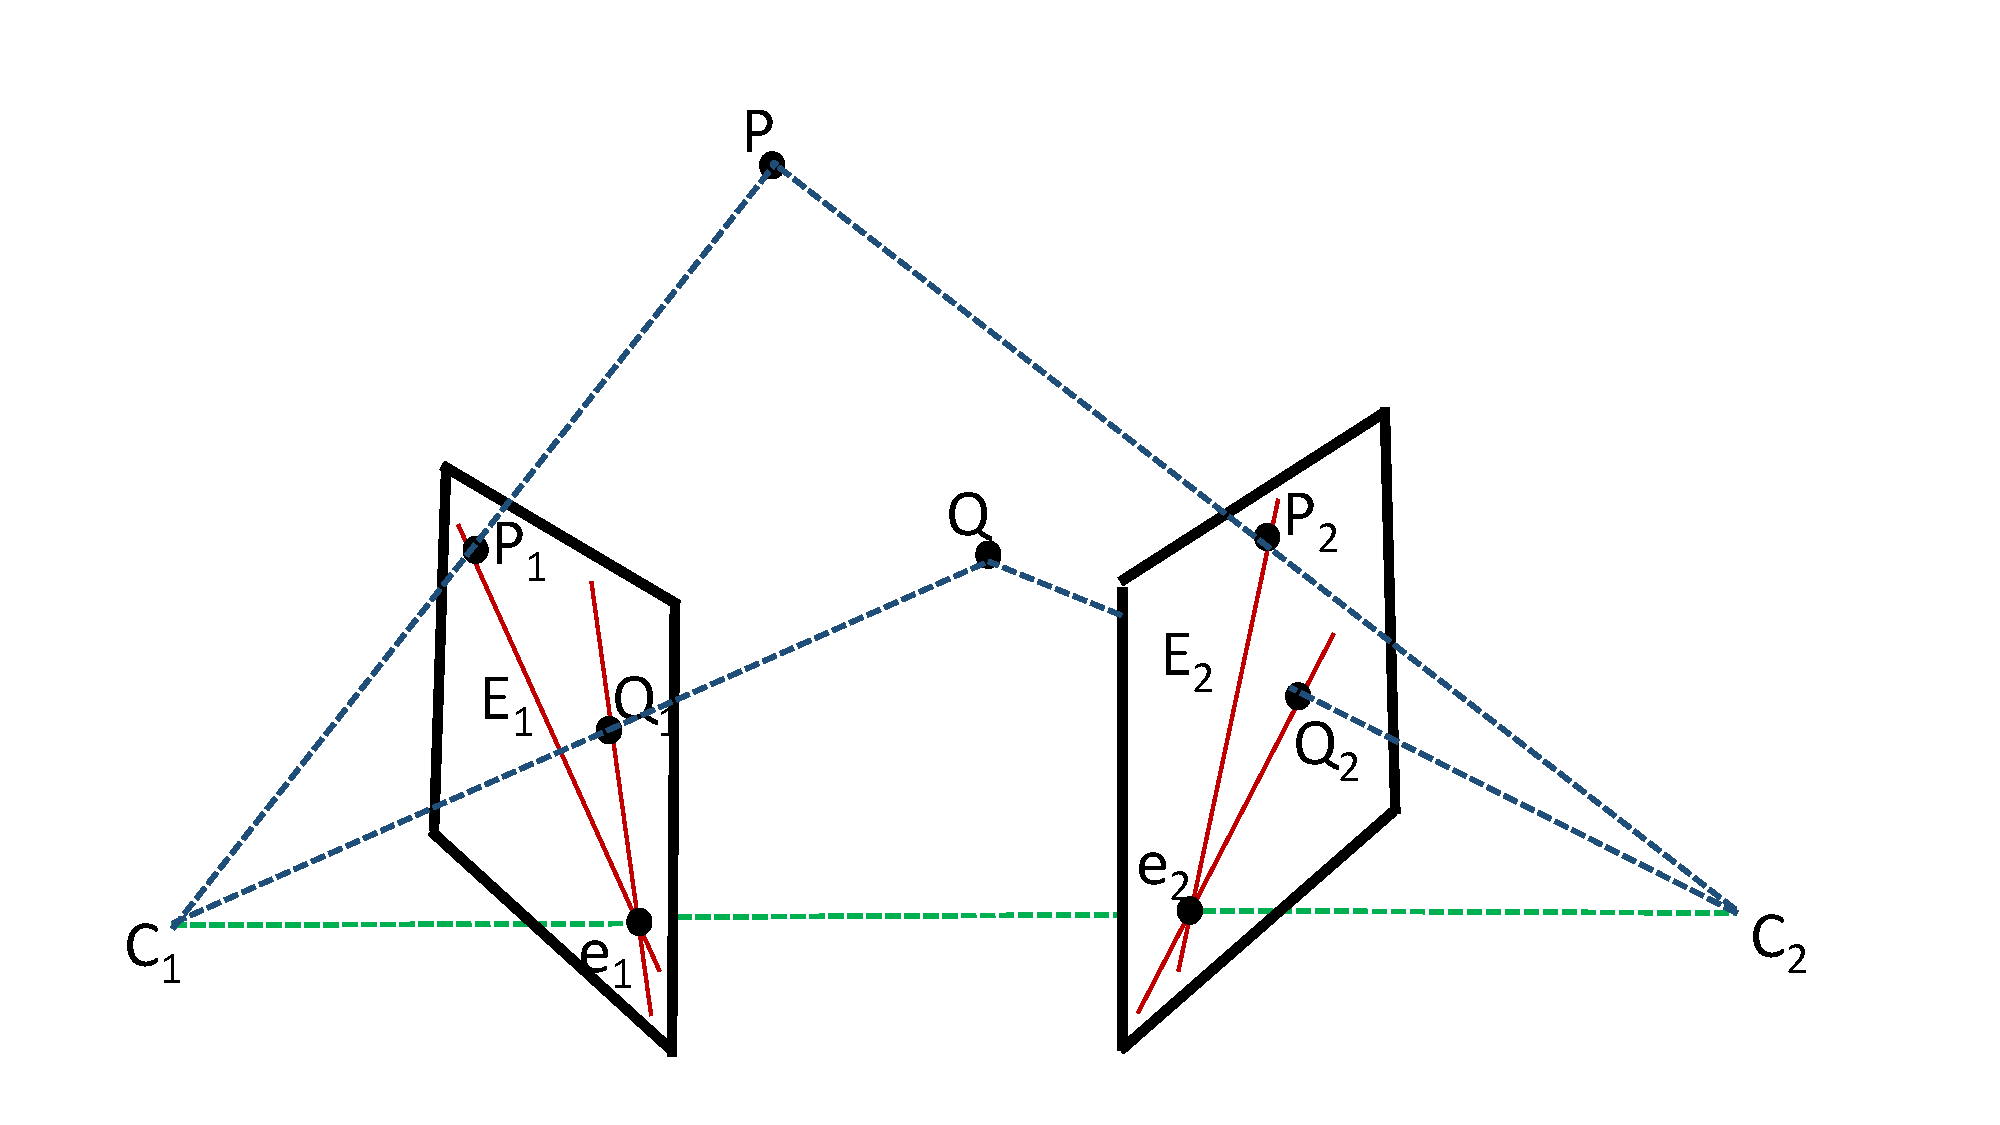
\includegraphics[width=5.0in]{images/introfm1}
	\caption{A pair of cameras viewing two points. This figure is a reconstruction of the figure on page 492 in Computer and machine vision: theory, algorithms, practicalities \cite{Davies12Computer}.}
	\label{fig:INTRO_FMA1}
\end{figure*}  

Using the steps described and looking at figure \ref{fig:INTRO_FMA1}, we now know how 3D point $P$ can be mapped to both of the frames with cameras $C_1$ and $C_2$. Projecting point $P$ onto the two frames gives points $P_1$ and $P_2$ respectively. Next, we describe the relation between vectors, $V_1$, formed by normalising the vector from $C_1$ to $P$, and $V_2$ (normalizing $(P - C_1)$. Skipping past the mathematical proof, which is detailed in Computer and Machine Vision \cite{Davies12Computer}, the relation between between these vectors is the essential matrix, $E$. This relation is $V_2^{T} * E * V_1 = 0$. Unfortunately we may not know the depth of $P$ and unless an investigation is performed on the particular camera system in use, we do not know the precise perspective transform and associated distortion. Fortunately, both the depth and the perspective are cancelled in this matrix formulation, and so we can specify the relation using only the 2D points, $P_1^T * E * P_2 = 0$. \\

This formula is based on the assumption that no distortion present in the camera system. In this case, both of the cameras may have distortion. We represent this distortion here using matrices $G_1$ and $G_2$. If both shots are taken with the same camera, we may assume $G_1 = G_2$. We therefore relate the theoretically precise $P_1$ and $P_2$ with their real world equivalents (which have distortion) $D_1$ and $D_2$ by $P_1 = Q_1^{-1} * D_1$ and $P_2 = Q_2^{-1} * D_2$. Inserting this into the essential matrix formulation we have, $(Q_1^{-1} * D_1)^T * E * Q_2^{-1} * D_2 = D_{1}^{T} * {Q_1^{-1}}^{T} * E * Q_2^{-1} * D_2 = 0$. The presence of this distortion is the difference between the essential and fundamental matrices with the fundamental matrix being $F = {Q_1^{-1}}^{T} * E * Q_2^{-1}$. If no distortion is present, the fundamental matrix is equivalent to the essential matrix. \\

Using the Essential or Fundamental matrices, we may compute both camera pose, and stereo calibration. If we take the essential matrix $E$ and break it down into 3 matrices ($W$, $U$ and $V$) using singular value decomposition (SVD). Here, translation may be computed using these matrices via equation \ref{eqn:FundaTrans} and the rotational part may be computed via equation \ref{eqn:FundaRote}


\begin{equation} \label{eqn:FundaTrans}
Translation Matrix = W\left[
\begin{array}{ccc}
0 & 1 & 0 \\
-1 & 0 & 0 \\
0 & 0 & 0 \\
\end{array}
\right]W^{T}
\end{equation}

\begin{equation} \label{eqn:FundaRote}
Rotation Matrix = W\left[
\begin{array}{ccc}
0 & -1 & 0 \\
1 & 0 & 0 \\
0 & 0 & 0 \\
\end{array}
\right]V^{T}
\end{equation}

Looking at figure \ref{fig:INTRO_FMA1} again, line $E_1$ represents something called an epipolar line, this line lies on the plane in which both cameras and point $P$ sit on. Line $E_1$ is the epipolar line of the left frame and $E_2$ is the epipolar line of the right frame. Point $e_1$ is the epipole of the left frame and point $e_2$ is the epipole of the right frame. Epipoles are the projection of one camera's location onto the frame of another camera. The projection of $C_2$ onto the left frame by camera $C_1$ is the epipole $e_1$. If the fundamental matrix is multiplied by a particular point it produces a vector in $R^3$ which represents the epipolar line as $[a b c]^T$ in which $a,b$ and $c$ represent the line equation $ax^2 + bx + c$. We can see that the epipolar line corresponding to $Q$ and $Q_1$ passes through a common point with the other epipolar line $E_1$. In fact, all epipolar lines intersect at the epipole. Therefore, if the fundamental matrix can be computed, so can the epipolar lines and the epipoles. \\

The fundamental matrix is computed using around 8 point matches between images. Using the fundamental matrix, image rectification can be performed as well as camera pose estimation. Using point $P$ in figure \ref{fig:INTRO_FMA1}, we already know the fundamental matrix, epipolar lines and epipoles can be computed from the point correspondences. If the epipoles are known, then we know the direction in which the other camera resides. The basic pipeline for the fundamental matrix method begins with feature matching, followed by fundamental matrix estimation via RANSAC. Then the extrinsic camera information is estimated and images are rectified and so that disparity information can be computed. Then depth maps can be projected through any of the two cameras and aligned. One downside to this method is that the scale of the translation computed is not to scale. \\


Monocular Feature based SLAM systems use feature matches to estimate camera pose and location changes across frames \cite{Davison02Simultaneous}. Variations of this method use different features including: corners and lines \cite{Jeong06Visual}, image patches \cite{Silveira08Efficient} and exemplar feature matching \cite{Chekhlov07Robust}. SIFT features are used most often in SLAM \cite{Jensfelt06Framework,Pollefeys08Detailed,Beall11Bundle,Eudes10Fast}, in addition FAST features have been explored \cite{Kundu10Realtime,Leelasawassuk133d,Konolige10View,Konolige08Frameslam}. Beall et al \cite{Beall11Bundle} made use of both SIFT and SURF features in their underwater SLAM system. Real-time monocular SLAM systems based on this approach have also been proposed \cite{Chekhlov07Robust,Pollefeys08Detailed}. RANSAC is often used in monocular SLAM \cite{Eudes10Fast,Kundu10Realtime,Konolige10View,Konolige08Frameslam,Pradeep13Monofusion} to remove outliers which cause incorrect camera parameter estimates. Bundle adjustment is also used as an additional step to refine camera parameter estimation \cite{Eudes10Fast}.  \\


\subsection{Feature Matching and RANSAC}
\label{FMANDFM}

Feature matching along with RANSAC  may be used to compute the Fundamental/Essential matrices which leads to camera pose estimates. However, the computation of the correct Fundamental matrix is typically difficult. Furthermore, the intrinsic camera parameters must be known prior in order to use such a technique, else noise destroys the ability to accurately estimate camera pose. \\

Another, more common way to use feature matching with RANSAC \cite{Fischler81Random,Chen99Ransac} is to compute the camera pose directly using RGB-D data. As covered in section \ref{DepthDataGenSection}, dense depth information may be computed using monocular, stereo or sensor based camera set-ups. This method begins by computing feature matches between two given frames. These matches along with the 3D location of each corresponding match (projected using the dense depth data) are injected into the popular Random Sample Consensus Algorithm commonly known as RANSAC. RANSAC is an iterative algorithm which works by repeatedly selecting a subset of input data, computing a model on the subset and testing that model on the global superset. During this repeated process, the subset with the best classification (lowest error or greatest strength model) is chosen for the final model. RANSAC is useful because it is capable of filtering out outliers. \\

In the case of camera pose estimation, the subset is used to compute the camera pose (using singular value decomposition) and the camera pose which minimizes the global error is chosen as the best camera pose. Here we describe how to compute the camera pose given a set of 3D points matched from one frame to another. Given two identical length arrays of 3D points, $P$ and $Q$ where, for each index $i$, $P_i$ matches best with $Q_i$. Next, we compute covariance matrix $X$ based on $P$, $Q$ and their mean values. The calculation for $X$ is shown in figure \ref{eqn:CovarMatForFMRansac}.


\begin{equation} \label{eqn:CovarMatForFMRansac}
X = \sum_{i=1}^{N} (P_i - P_{mean}) \times (Q_i - Q_{mean})^T
\end{equation}

Given the covariance matrix $X$ we compute its singular value decomposition matrices $W$, $U$ and $V$ (was usv). Then the rotation part of the pose may be computed as $R = V^T \times U^T$. The camera movement can be computed by $T = -R \times P_{mean} + Q_{mean}$. If scale must be computed, it can be computed as $S = (Q_i - Q_{mean}) / (R \times(P_i - P_{mean}))$ for any $i$. \\

Computing 3D reconstructions using feature matching is often preferred as close competitor ICP (Iterative Closest Point) is often unnecessary and expensive \cite{Endres12Evaluation}. However, the computation of pose without ICP with feature matching only is non-trivial because the system may suffer from the following issues:


\begin{itemize}
\item Synchronization problems between the RGB camera and Infrared camera shutters
\item depth jump interpolation - the interpolation of computed depth at object boundaries
\item feature matches often occur at depth jumps
\end{itemize}



\subsubsection{RGB-D SLAM}

Endres et al \cite{Endres12Evaluation} presented a dense 3D reconstruction technique using RGB-D data from the Kinect sensor based on feature matching and RANSAC. They also evaluated their technique under different illumination and camera movement speed conditions. It is able to operate at near real time speeds in small in-door environments. This method begins by feature matching RGB images across frames. Using the projected 3D points available for each pixel in the depth map, RANSAC \cite{Fischler81Random,Huttenlocher91Fast} is used to compute the camera pose across frames. These poses are optimized globally using the $g^2$o graph optimizer, the Octomap representation \cite{Wurm10Octomap} is used to voxelize the 3d points before storing them in a volumetric occupancy map. Since this system is based on feature matching, Endres et al evaluate 3 different feature matching techniques: SIFT \cite{Lowe04Distinctive} , SURF \cite{Bay06Surf,Bay08Speeded} and ORB \cite{Rublee11Orb}. ORB feature matching is tested because it is faster than SIFT and SURF with slightly less accuracy, the authors also evaluate a GPU implementation of SIFT \cite{Wu07Siftgpu}. Endres et al evaluate their algorithm using their own benchmark \cite{Sturm11Towards}. Results show it can handle up to 50 degrees of rotation per second, and speeds of up to 43 centimetres per second.  \\


This system is divided into a front-end and a back-end. The front-end performs feature detection, matching and sensor pose estimation via the RANSAC method whereas the back-end performs non-linear pose optimization using the $g^2o$ optimization procedure   and integrates these results into an occupancy grid based on the Octomap. A diagram of the combined front-end and back-end systems is given in figure \ref{Endres12EvaluationPipeline}. 


\begin{figure}[!h]
\centering
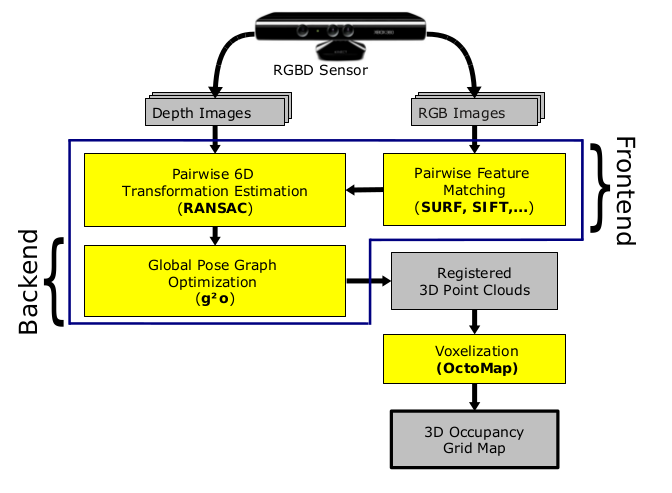
\includegraphics[width=12cm]{images/ch1/Endres12EvaluationPipeline}
\caption{RGB-D SLAM Pipeline used by Endres et al \cite{Endres12Evaluation}}
\label{Endres12EvaluationPipeline}
\end{figure}


The front-end uses OpenCV \cite{Bradski08Learning} for feature matching. During the feature detection process, the Hessian threshold is used to keep the total number of features constant. This is required because pose may not be able to be computed if there aren't enough features, but on the other hand, too many features typically lead to many false positives in the feature matching schema. As mentioned, these matched features (and thus matched 3d points) are used with RANSAC to compute pose \cite{Umeyama91Least}. During the RANSAC process, corresponding points with distances below 3cm are considered inliers. The inliers are then used exclusively to compute a finer pose. This method of pose estimation is fast but computational complexity depends on the number of features computed. For each frame, the pose relationship with 20 previous frames (including the most recent 3) is computed in parallel on the GPU. Then the final computed pose is given to the back-end. If accurate pose cannot be compute, constant motion is assumed. \\

\subsection{ICP}

Iterative Closest Point (ICP) \cite{Besl92Method,Rusinkiewicz01Efficient,Segal09Generalized} is a non-linear optimization method used to register 3D data. It works by iteratively minimizing registration error given two sets of point clouds and is a popular method for estimating 6-dof (6 degrees of freedom) camera alignment in 3D reconstruction. The algorithm works by computing the closest point using some metric (usually euclidean distance) for each of the points in the first point cloud. Then computing a transform which minimizes either the euclidean distance error or some other error metric (\cite{Steinbrucker11Real,Tykkala11Direct,Kerl13Robust,Chen92Object}. \\

The points are then transformed by the computed transform and this process is repeated which is supposed to continually decrease registration error. The 6-dof are commonly computed using the method described in section \ref{FMANDFM}. Various distance metrics have been researched including the point-plane metric \cite{Chen92Object}. This metric improves convergence rates and is used for surface reconstructions which contain additional information about the normal of each points. This algorithm is highly successful in generating accurate 3D reconstructions but it does have a few issues. \\

The first issue is that whilst computing the best transform based on "feature matches" based on closest points is relatively simple, computing these closest points for each input point is expensive. This can be improved using the projective data association algorithm \cite{Blais95Registering} usually used by exploiting a projected version of the 3D data. The efficiency issue can also be improved using a coarse to fine scheme. \\

Another issue that ICP is limited to small rotation, translation and scale. If larger transforms are present (especially scale in the case of general registration) ICP will usually get stuck in a local minima and fail to register \cite{Mitra04Registration}. Here we present some important algorithms which use ICP in 3D reconstruction.

\subsubsection{Henry10Rgb}

Some systems make use of feature matching with RANSAC (see section \ref{FMANDFM}) for pose estimation and ICP for further alignment \cite{Engelhard11Real, Henry10Rgb}. These methods are very similar and make use of the advantages of both the feature matching methods and ICP method. \\

Henry et al \cite{Henry10Rgb} presented work on a 3D mapping method which combines Feature Matching and RANSAC (similar to \cite{Endres12Evaluation}) with ICP. This method makes us of an RGB-D camera, and used the camera input for sparse feature matching. Features are used with RANSAC and the technique described in section \ref{FMANDFM}. ICP is used for refinement of the initial prediction. If Loop-closure is detected, a constraint is added to the 3D pose graph \cite{Kummerle11G} and is used to close the loop. A Surfel \cite{Pfister00Surfels} volumetric fusion method is used to represent and store the 3D reconstruction. This technique may be used for robot localization and path planning \cite{Hornung10Humanoid}. Endres et al \cite{Endres12Evaluation} compared this method with theirs using a standard benchmark \cite{Sturm12Benchmark}.  \\

\subsubsection{Non-Rigid Alignment}

In addition to rigid alignment ICP is used by Pauly et al \cite{Pauly05Example,Brown07Global} to 
non-rigid alignments:
	Pauly et al. 2005 \cite{Pauly05Example}
	Brown and Rusinkiewicz 2007 \cite{}
	
ICP used, then global feature positions are found using a relaxation method 
the 3d point sets are then warped to final positions using thin plate splines.

outperforms rigid based alignments


\subsubsection{Kinect Fusion}

Newcombe et al \cite{Newcombe11Kinectfusion} proposed an accurate, real-time dense 3d reconstruction algorithm which works well on complex indoor environments. This algorithm computes relationships between depth map frames generated using the Microsoft Kinect \cite{Zhang12Microsoft} sensor. By aligning depth maps this method is capable of tracking both camera pose and location as well as generating dense 3d reconstructions. Only depth data is used in alignment computations thus, consequently because the Kinect is a structured light based depth sensor Kinect Fusion works under any lighting condition, including complete darkness. Since they use the Kinect and GPU (both considered commodity hardware these days) the technique may be considered inexpensive. \\

The method works by computing camera pose, transforming depth data by a computed pose (frame-by-frame) and fusing this data into a global surface volume. It uses a coarse to fine grain iterative closest point (ICP) algorithm to compute camera pose. During the ICP phase, the target points come from the entire globally matched previous frames. Therefore this method is considered global rather than frame-to-frame based. Such a method has direct advantages over frame-by-frame feature matching, since all data is used to compute pose. The downside, is that this method fails to find global solutions due to the nature of ICP. This may occur when some frames must be skipped due to motion blur, or the camera passing over surfaces which do not reflect infra-red light. \\

\begin{figure}[!h]
\centering
%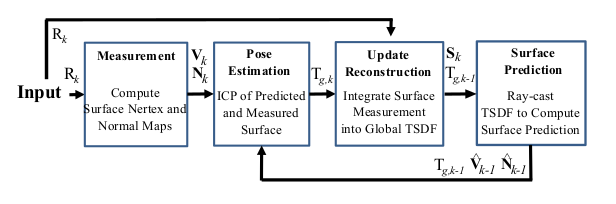
\includegraphics[width=12cm]{images/ch1/Newcombe11KinectFusion1}
\caption{Kinect Fusion Algorithm Pipeline \cite{Newcombe11Kinectfusion}}
\label{KFusionPipeliciteHne}
\end{figure}

Kinect Fusion has four main steps as illustrated in figure \ref{KFusionPipeline}. The first step named measurement, performs pre-processing on the depth data as well as generation of additional information for use by Kinect Fusion. Each depth map frame is first passed through a bilateral filter. From this, a dense vertex map (map of 3D points projected using a known projection matrix associated with the Kinect) is generated, as well as a normal map. For both the vertex and normal maps, a 3 level image pyramid is constructed. This makes the coarse to fine grain ICP technique possible. \\

Next, dense coarse to fine grain ICP is used to compute pose between the fused frames and the current frame. The authors exploit the fact that the transformation between frames is small because camera motion is slow when computing against every frame. With coarse-to-fine grain ICP they use projective data association \cite{Blais95Registering} and the point-plane metric for pose optimization \cite{Rusinkiewicz02Real}. The ICP based pose estimation computes pose given both a predicted and measured depth map. \\

After estimating camera pose relating to the globally fused model, each frame must be integrated into that model. The Kinect Fusion algorithm uses a truncated signed distance function (TSDF) representation. This is a signed distance function volume where the distances for each voxel are capped by some value. The TSDF uses a volume resolution of $512\times 512\times 512$. They use the TSDF, rather than relying on a linear but accurate discrete SDF transform \cite{Rasch09Remarks} because of the computational complexity of calculating the discrete SDF of large scale volumes. \\

As mentioned, Kinect fusion uses pose prediction and fuses each depth map into the TSDF representation. In this way, they align and fuse each depth map to the global 3d reconstruction. In this way, a global loop closure method is not required. This may have a negative side effect by which some frames which have larger resolutions may be heavily quantized in order to fuse with the SDF, especially very thin surfaces/objects. These features may also be advantageous for ICP in estimating pose. 


\subsection{SDF Optimization}

In 2013, Bylow et al \cite{Bylow13Real} presented a novel method which reconstructs static indoor environments in real time using RGB-D data captured using the Asus Xtion Pro Live sensor. Their system is able to generate accurate 3D RGB coloured models of the environment in real-time by optimizing for 6 degrees of freedom in terms of accurate projection of new depth map frames into an existing global signed distance function model of the scene. Their method uses several Gauss Newton optimization with a signed distance function representation, these techniques are represented and processed using a laptop with an NVIDIA GPU. Unlike Kinect Fusion \cite{Newcombe11Kinectfusion}, this method optimizes directly in the signed distance representation, in which camera pose is computed by finding a rotation and translation (6-DoF) which minimizes the error of projecting depth images into the SDF. Compared with the ICP based method used by Kinect Fusion, this technique is shown to be more robust and accurate. It compares favourably to bundle adjustment but is much faster for small to mid sized scenes. Results are generated using the TUM RGB-D benchmark and SDF volume sizes $256^3$ and $512^3$ are used in evaluations. The authors note the algorithm may be able to handle large scale scenes if used in conjunction with other techniques \cite{Kaess11Isam2,Kummerle11G}. \\

This technique is efficient because the error to minimize can be checked using several look-ups since the SDF itself contains the distances from each voxel to the global model's actual surface. Because of this, the algorithm is classified as working within global space rather than frame-by-frame. Using the SDF to lookup depth map projection error, the camera pose is iteratively estimated and then the depth map is integrated into the SDF and colour information is stored in another volume. The pose estimation procedure begins by storing the first frame as a volumetric signed distance function. Then for each new depth frame, camera pose is computed, and based on this pose the frame is projected into the scene. Using a lie algebra based 6-DoF model \cite{Ma12Invitation} envisioned as a vector in $R^6$ representing camera pose, the error for a given pose may be computed as the squared error of the depth map transformed by the pose and projected into the signed distance function. Due to noise or missing data within the depth frame, this error may never be reduced completely, instead the best pose is iteratively computed using this model and the Gauss Newton non-linear optimization algorithm. \\

The SDF representation uses two volumes as in \cite{Curless96Volumetric}, one volume stores the average distances, the other stores the cumulative weights for each voxel. Bylow et al use these weights to handle occlusion and sensor uncertainty. When integrating a point into the SDF, tri-linear interpolation is used between eight neighbours to handle point coordinated made up of floating point numbers. During integration, each voxel is projected onto the image plane rather than ray case from the center of projection as in \cite{Newcombe11Kinectfusion}. This ensures that each voxel is visited once when updating the SDF, whereas in the ray casting approach, this may not necessarily be the case. \\

In computing the SDF for a given depth map, the exhaustive marching cubes algorithm is too slow, even the fast marching algorithm \cite{Baerentzen01Implementation} is not suited for real time discrete SDF generation. Instead, the SDF is approximated with either the point to point distance or point to plane distance functions. For final visualization, marching cubes is used \cite{Lorensen87Marching} on the final SDF. Colour is computed from the colour volume using a technique found used by Whelan et al \cite{Whelan13Robust}. Since the method by Bylow et al is based on optimizing the projection error using the SDF and only uses locations in its pose estimation procedure, it is independent to illumination. Given this, it will also fail in cases where only co-planar surfaces are visible, they mention that using colour information during tracking \cite{Kerl13Robust} may mitigate these concerns.


\subsection{3D Feature Matching}

3D feature matching works much in the same way as the 2D feature matching and RANSAC approach (section \ref{FMANDFM}) but uses 3D features rather than 2D only, so it can work independently to perspective changes which 2D feature matching methods are only robust to. Many techniques have been proposed \cite{Scovanner073Dimensional,Flitton10Object,Li05Multiscale}. Technically, registering against rigid transformations may be achieved with as little as 3 feature matches. These 3 matches can be found by 3D feature matching or geometric hashing \cite{Wolfson97Geometric}.



\subsubsection{4-Point Congruent Sets}

Aiger et al \cite{Aiger084} developed a method for 3D registration (and pose estimation) named 4-Point Congruent Sets (4-PCS). This method is fast and robust to wide baselines in the registration of 3D data. It is resilient to noise and outliers and there is no pre-filtering or de-noising required prior to registration. It improves the typical feature matching approach by significantly reducing the number of points required to compare as features for use in a RANSAC approach to pose estimation. \\

This method works by extracting all co-planar 4 point sets from a 3D point cloud which are congruent (under a rigid transformation) to a given set of co-planar 4-points. The complexity of this method is $O(N^{2k})$ where N is the number of points and k is the number of 4-point sets. When there is not too much noise, this method may use feature matching only which brings the complexity down to $O(N+k)$. Aiger et al also presented an extension to register against affine transforms. This method was tested with varying levels of noise, outliers and and overlap. \\

This method works based on the principal of large numbers, which means solving the largest common point-set (LCP) problem. This problem states, given to point-sets $P$ and $Q$, LCP under δ-congruency solves for a subset $P_i$ of $P$ having the largest cardinality such that the distance between $T(P_i)$ and $Q$  is less than δ given an appropriate distance measure (T is a rigid body transformation). \\

The basic concept is to optimize the selection of the 3 points used as a base for alignment from one point-set to another. By choosing 3 matches, then measuring the distance between $T(P_i)$ and $Q_i$. This test is of complexity  O($m^3$ x $n^3$) but this can be reduced to  O($mn^3 log(n)$) \cite{Irani96Combinatorial} and even O($n^3 log(n)$). Despite these improvements, these complexities are still too large for practically sized point-sets. This novel 3D alignment scheme is capable of aligning surfaces with limited overlap and may be refined using ICP \cite{Rusinkiewicz01Efficient}. \\


\subsubsection{Base Shape Matching}

Gelfand et al \cite{Gelfand04Shape} presented a method which segments input models into base shapes, simple geometric parts which may be modelled and matched. Using these base shapes, slippable components are found by computing local slippage signatures for a set of points in the input and iteratively clustering regions with matching slippable motions. This method is stable but appears to be limited to mechanical human made parts and shapes.

\subsubsection{Multi-scale Features}

Extensions to both SIFT and SURF have been extended to 3D \cite{Scovanner073Dimensional,Flitton10Object}. These methods follow the same overall technique as the 2D counterparts however some procedures and practices are altered to better suit 3D data input. First, a 3D-volume scale pyramid is produced for matching at different scales. Then features are detected using the corresponding feature detection method (by SIFT or SURF) and then a feature vector for each feature is produced. Features can be matched between volumes and a rigid or non-rigid alignment may be computed. \\

Li and Guskov \cite{Li05Multiscale} developed a 3D feature matching technique based on 3D SIFT for SURFEL (3D point and normal) data. It computes a scale space pyramid using a per point scheme in which the next scale up for each point and corresponding normal is computed as the point which minimizes an error function. Salient features are then computed using the scale space. Features are those points which maximize (or minimize) a measurement based on dot product of the normal and the difference between points at adjacent scales. \\

Li and Guskov use their technique to find approximate transformations, then ICP is used for further alignment \cite{Besl92Method,Chen92Object}. This technique is slow for data-sets with large amounts of input data, yet it does not work well with sparse data-sets. \\

	
Mori et al \cite{Mori05Efficient} proposed a matching method based on two levels: a high level matching method which is used to compute a short-list for candidates and a low level method which is more computationally complex. This technique is simply used for matching and uses larger areas rather than local features like SIFT 3D. \\

Other 3D feature matching techniques which have been developed are based on images \cite{Wolfson97Geometric,Johnson97Spin}. In these techniques features are typically described using some sort of 2D image function rather than a single dimensional vector. Typically a normal is computed for a feature point and some projection is used to compute an image which is used as a descriptor. Then these features may be matched between 3D volumes using normalized cross-correlation or another image comparison method.  \\



\subsubsection{Hashing Techniques}

hashing-versions:
	[Germain et al 97 \cite{Germain97Fingerprint}
	Gal and Cohen-Or 06 \cite{Gal06Salient}
	Mitra 06 \cite{Mitra04Registration}]


voting rather than ransac
	[Ballard 87 \cite{Ballard91Generalizing}]

\subsection{Principal Components Analysis}

PCA can be used to compute bases but in the case of partial overlap, this quickly breaks down \cite{Aiger084}

	Pottmann et al. 2007 \cite{Pottmann07Principal}
		shows that PCA on local neighbourhoods can be used to define pricipal directions and curvatures at a given scale (this can be used for feature matching



%optimization techniques
\section{Global Optimization}

\subsection{$G^2$o}

graph slam use motion estimates as input to construct and optimiza a pose graph[15 \cite{Kummerle11G}] these methods render a joint map only after pose graph optimization
this map is generally not used for further optimization
the resulting maps are often represented as occupancy grid maps or octrees [25 \cite{Wurm10Octomap}]




\subsection{Bundle Adjustment}

Fioraio [7 \cite{Fioraio11Realtime}] presented a system which uses bundle adjustment to align rgb-d data


bundle adjustment using features over many views with [13 \cite{Klein07Parallel} , 2 \cite{Agarwal09Building}] with sparse 3d models generated

[END BUNDLE ADJUSTMENT]



[BG Bylow]

? not sure where to put this yet [maybe icp...]
whelan [24 \cite{Whelan13Robust}] estended with rolling reconstruction volume and color fusion, evaluated alternative methods for visual odometry estimation
pure visual odometry induces significant drift, so matching with global model is their preference
whelan integrated photometric + icp methods for kinect fusion [24 \cite{Whelan13Robust}]
?






\ref{Newcombe11Kinectfusion}

\subsection{RGB-D Sensor Feature Based Systems}
RGB-D SLAM systems use both depth and image data and are capable of generating dense 3D reconstructions. Many of these methods rely on feature matching techniques \cite{Engelhard11Real,Henry10Rgb,Endres12Evaluation}. RANSAC is often used to filter outliers for the estimation of camera parameters\cite{Engelhard11Real,Henry10Rgb,Endres12Evaluation}. Another method which has also been used extensively in the area is Iterative Closest Point (ICP) \cite{Engelhard11Real,Henry10Rgb,Bylow13Real,Newcombe11Kinectfusion,Stuckler12Robust,Izadi11Kinectfusion}. ICP iteratively registers point cloud data, and is used to refine camera parameter estimates. A method named KinectFusion was proposed by Newcombe et al \cite{Newcombe11Kinectfusion} which uses RANSAC and a GPU implementation of IPC. Whelan et al \cite{Whelan12Kintinuous} extended this method allowing it to map larger areas using Fast Odometry From Vision (FOVIS) over ICP. Bylow et al \cite{Bylow13Real} improved the ICP approach by registering data using a signed distance function.
\subsection{Non-Feature Based Methods}
Several RGB-D SLAM systems are also non-feature based \cite{Weikersdorfer14Event,Izadi11Kinectfusion,Kerl13Dense}. Weikersdorfer et al \cite{Weikersdorfer14Event} presented a novel sensor system named D-eDVS along with an event based SLAM algorithm. The D-eDVS sensor combines depth and event driven contrast detection. Rather than using features, it uses all detected data for registration. Kerl et al \cite{Kerl13Dense} proposed a dense RGB-D SLAM system which uses a probabilistic camera parameter estimation procedure. It uses the entire image rather than features to perform SLAM.
\subsection{Summary}
As is evident from the current literature, SLAM typically relies on feature matching and RANSAC. However, these approaches fail when there are too few features, when feature confusion occurs or, when features are non-stationary due to object motion. As the extent of random feature displacement becomes more global the effectiveness of these approaches diminishes. Feature matching also dominates in image registration. However, Fourier based methods have been shown to work well under larger rotations and scales \cite{Gonzalez11Improving} whilst being closed form, insensitive to object motion and scaling naturally to GPU implementations. Accordingly, we propose a novel, closed form Fourier based SLAM method.

Simultaneous localization and mapping (SLAM) has applications in many fields including: robotics, business, architecture and engineering, and science. Its goal is to generate a map (2D birds-eye view, or 3D) of an environment captured by camera and/or other means. In this work we focus on monocular systems, or systems which generate location and mapping data using information generated by a single basic video camera. To this end, current methods rely on the computation of the fundamental and essential matrices. These feature matching techniques fail in cases where features are not stable or where feature confusion occurs. 

It has been shown [1] that using volume registration to compute dense 3D maps is not only independent of feature matching, but it is a closed form solution and is robust to noise and object motion. However, this method requires RGB-D video input provided by special hardware. In this paper we present preliminary results in applying volume registration to generate dense 3D maps from monocular video data. To achieve this, disparity maps are generated between video frames. This data is then used as input for the RGB-D volume registration method.


%data compression and representation
\section{3D Reconstruction Data Representations}

\subsection{Mesh}

Mesh data is popular due to its simplicity and integration into GPU technology. The 3D data is made of connected polygons which in turn are made of vertices. Edge information is typically defined implicitly. An example can be seen in figure \ref{MeshExamples}, vertices are represented using black dots, edges by lines, and polygons are labelled $F_0, F_1, F_2, F_3, F_4$. Here, vertex data define geometric information whilst edge and polygon data forms topological information. \\

For processing purposes, polygons are usually triangulated, which means all polygons are sub-divided into triangles. Any mesh may be triangulated, an example of this is provided on the right hand side in figure \ref{MeshExamples}. In a typical data representation, vertices are stored in a list and triangles are stored using three references to this list. The number of bits per vertex (bpv) is typically used to measure storage requirements for mesh data. \\

\begin{figure}[!h]
\centering
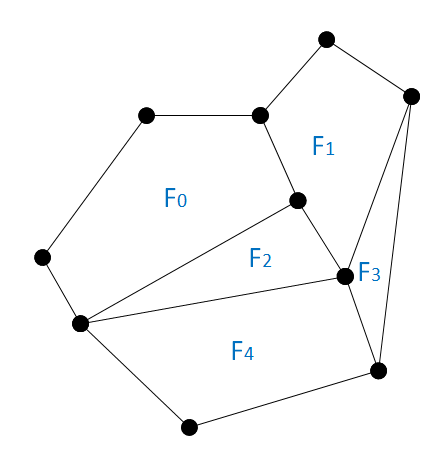
\includegraphics[width=6cm]{images/ch2/PolygonMeshExample}
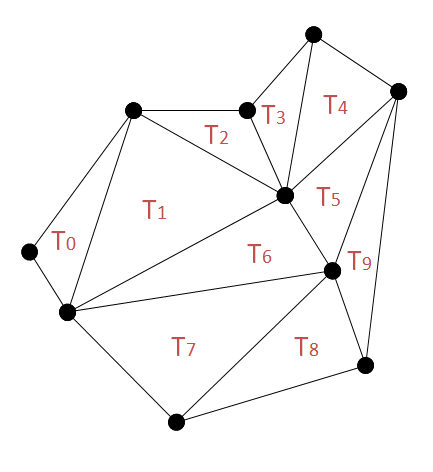
\includegraphics[width=6cm]{images/ch2/TriangleMeshExample}
\caption{Left: Polygonal Mesh, Right: Triangulated Mesh}
\label{MeshExamples}
\end{figure}

\subsection{The Point Cloud Representation}

The point cloud structure stores a list of 3D points. This representation can be thought of as discrete samples of the surface of a real 3D object. Figure \ref{PointCloudExample} shows an example. This structure can be sampled using a variety of methods. These methods include both dense and sparse sampling, and sample steps can be either regular or irregular. Along with each vertex, a variety of attribute information can be stored. Point cloud data may be obtained via a 3D scanner or RGB-D camera. 

\begin{figure}[!h]
\centering
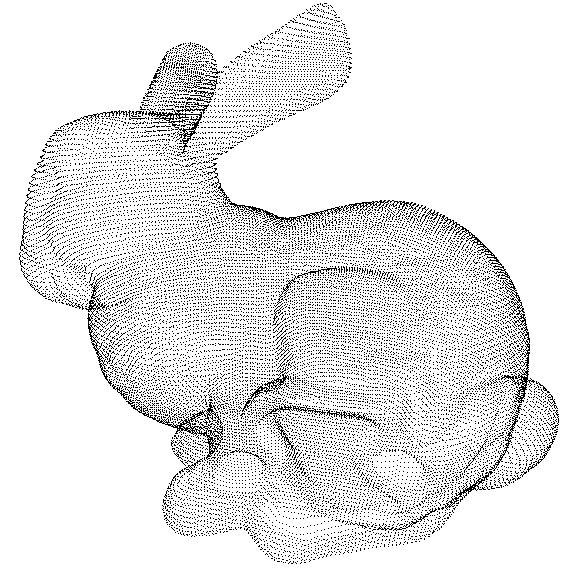
\includegraphics[width=6cm]{images/ch2/PointCloudExample}
\caption{A densely sampled point cloud of the Stanford Bunny.}
\label{PointCloudExample}
\end{figure}


\subsection{3D Volume}

In this representation, points are sampled into a 3D cubic space of sub-cubes called voxels. Such a space may have separate sizes for width, depth and height or the space may be a true cube. In the context of 3D reconstruction, this data-representation is common and is used to store boolean values describing the occupancy of a space \cite{Rusinkiewicz02Real}. A visualization of a 3D volume showing a reconstruction is shown in figure [WARNING: Insert Graphic here]. This data type is useful because it allows for quick updates. Downsides include: large storage space and the 3D space represented cannot be dynamically changed without significant cost.

\subsection{Signed Distance Functions}

A Signed Distance Function \cite{Curless96Volumetric} is a function which describes a 3D geometric space. Such a function takes a 3D location as $x,y,z$ coordinates as input and returns a single number value. The value describes the geometric detail of a particular object. Zero values are surface interfaces, positive values increase relative to the distance to the nearest surface and negative values represent the interior of the object. \\

SDFs may take the form of an equation or may be made discrete by means of discretization. In the context of 3D reconstruction we refer to the discrete SDF and example of which is show in figure [WARNING : insert a figure]. The SDF may be visualized by converting to mesh and rendering (by means of the marching cubes algorithm \cite{Cubes87High}) ray cast directly \cite{Parker98Interactive}. In the case of ray-casting a significant advantage over the volumetric representation, that is the step size may be adjusted dynamically reducing render time. \\

Canelhas \cite{Canelhas12Scene} did a masters thesis on an approach for camera tracking which makes use of an SDF. Similar to the work by Bylow et al \cite{Bylow13Real} the project concentrates on object detection and recognition in an SDF although little evaluation was performed. Additionally storage was not considered. Kubacki \cite{Kubacki12Registration} proved the SDF is useful in estimating camera pose but only showed proof using synthetic data performing no comparative evaluation. Ren and Reid \cite{Ren12Unified}  demonstrated SDF based object tracking based on prior known models. \\

[WARNING check these citations first:::]
Elfes et al \cite{Elfes87Sensor} use a Baysian probability of occupancy measure to decide if a point should be added to the grid and showed that SDFs can be used to fuse partial depth scans whilst impeding problems with mesh based reconstruction algorithms. The SDF representation was modified by Zach et al \cite{Zach07Globally} to be more robust to noise. Bylow et al noted that the SDF may be used for real time processing and produce globally satisfied reconstructions.


\subsection{Image Based Representations}

3D reconstructions may also be represented by means of elevation maps [7] and multi-level surface maps [19] however these methods cannot store known and unknown areas of occupancy in a volumetric way. Additionally compression is often not considered and these methods do not have the search capabilities which the Octree and volumetric representations have, nor the fine detail available in a mesh or point cloud representation. An example of an elevation map is shown in figure [WARNING: insert figure here]


\subsection{Octree}

The Octree is a hierarchical data representation ideal for storage, search and processing of 3D data. Other hierarchical structures exist (such as K-D tree and BSP-tree) \cite{Samet06Foundations} but these are not as useful for compression as the Octree, which is the aim of this research. The Octree is described in detail below in section \ref{OTDesc}. An important technique based on the Octree and used by many 3D reconstruction methods is the Octomap \cite{Wurm10Octomap}. It essentially records a volume occupancy grid using an Octree. This method models data probabilistically whilst simultaneously reducing memory size. The Octomap representation is lossless and is can reduce the file size of the reconstruction by up to 50\%. \\

Other methods also explore the Octree for 3D reconstruction and SLAM \cite{9,Fournier07Mapping,Meagher82Geometric,Fairfield07Real} however these methods do not really address storage advantages. 



\subsubsection{Octree Description}
\label{OTDesc}

In order to understand the OT structure, the Quad-Tree (QT) is explained first. This is done because the QT is the 2D equivalent of the OT and is easier to explain. The QT is a hierarchical data structure used for processing and compressing 2D data. Figure \ref{QuadtreeExample} shows an example of a QT used to represent an image. In this figure, the original image is on the left. The QT first uses a single coloured square to represent the entire image, then using some error metric it decides whether or not to, a) represent the image more accurately using more memory or b) stop decomposition and represent the image with a single colour. If option b) is chosen, the image will look like the second left picture. If option a) is chosen, the image is divided into four sub-images each with its own colour. From here the whole process begins again, with each sub-image given the same options. The final product of the QT is shown on the far right in figure \ref{QuadtreeExample} and a visualization of a QT hierarchy is shown in figure \ref{QuadTreeHierarchy}.
\begin{figure}[!h]
\centering
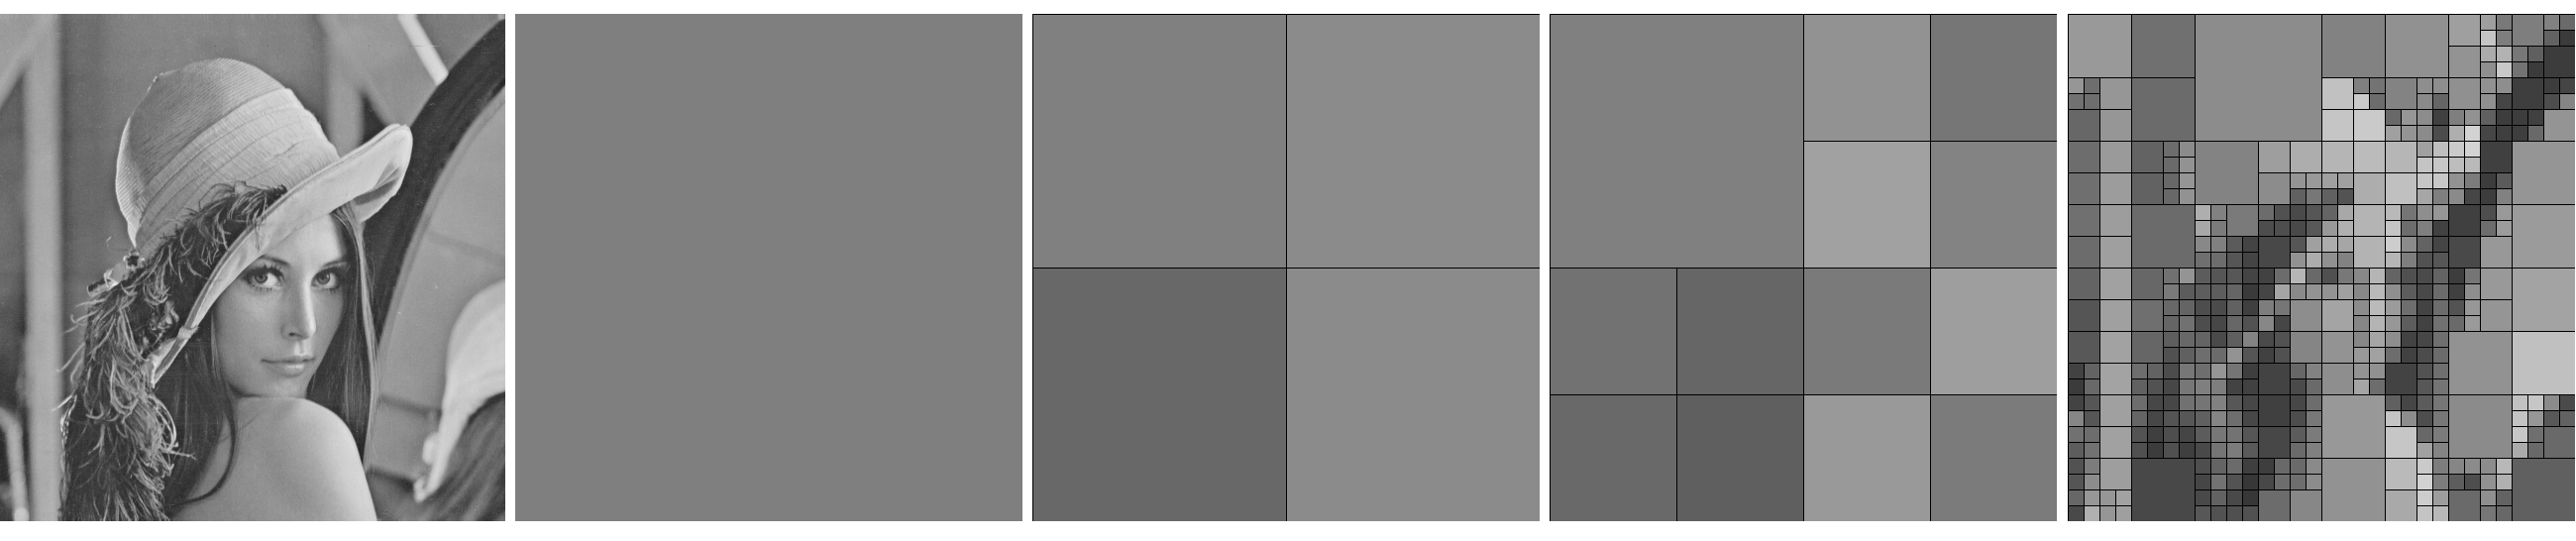
\includegraphics[width=12cm]{images/ch2/quadtreeexample}
\caption{Quadtree Image Representation, left to right: Original Image, 1st Level of Decomposition, 2nd Level of Decomposition, 3rd Level of Decomposition, QT codec Image.}
\label{QuadtreeExample}
\end{figure}
\begin{figure}[!h]
\centering
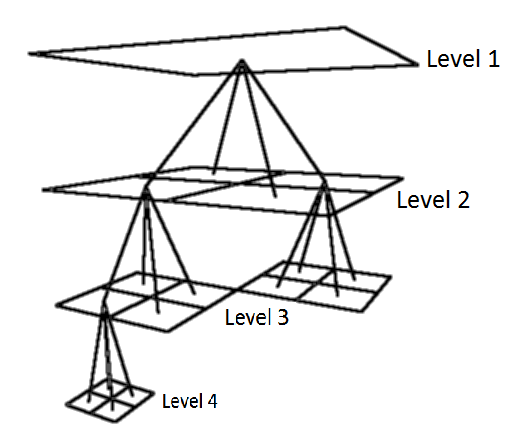
\includegraphics[width=6cm]{images/ch2/QuadTreeHierarchy}
\caption{A visualization of the QT hierarchy}
\label{QuadTreeHierarchy}
\end{figure}

The OT works similarly to the QT, however, instead of beginning with a square encompassing the entire region, a cube is used to enclose a 3D space. Similarly to the QT, an error metric is used to decide whether to split up the space or leave it unchanged. Each split operation divides each coordinate ($x,y,z$) by two, leaving 8 subspaces. Figure \ref{OctreeExample} shows this decomposition. The further each cube is split, the more the OT resembles the model being compressed. In the QT and OT, nodes which have not been split are called leaf nodes and the function which decides whether a node should be split is called the leaf criterion. 

\begin{figure}[!h]
\centering
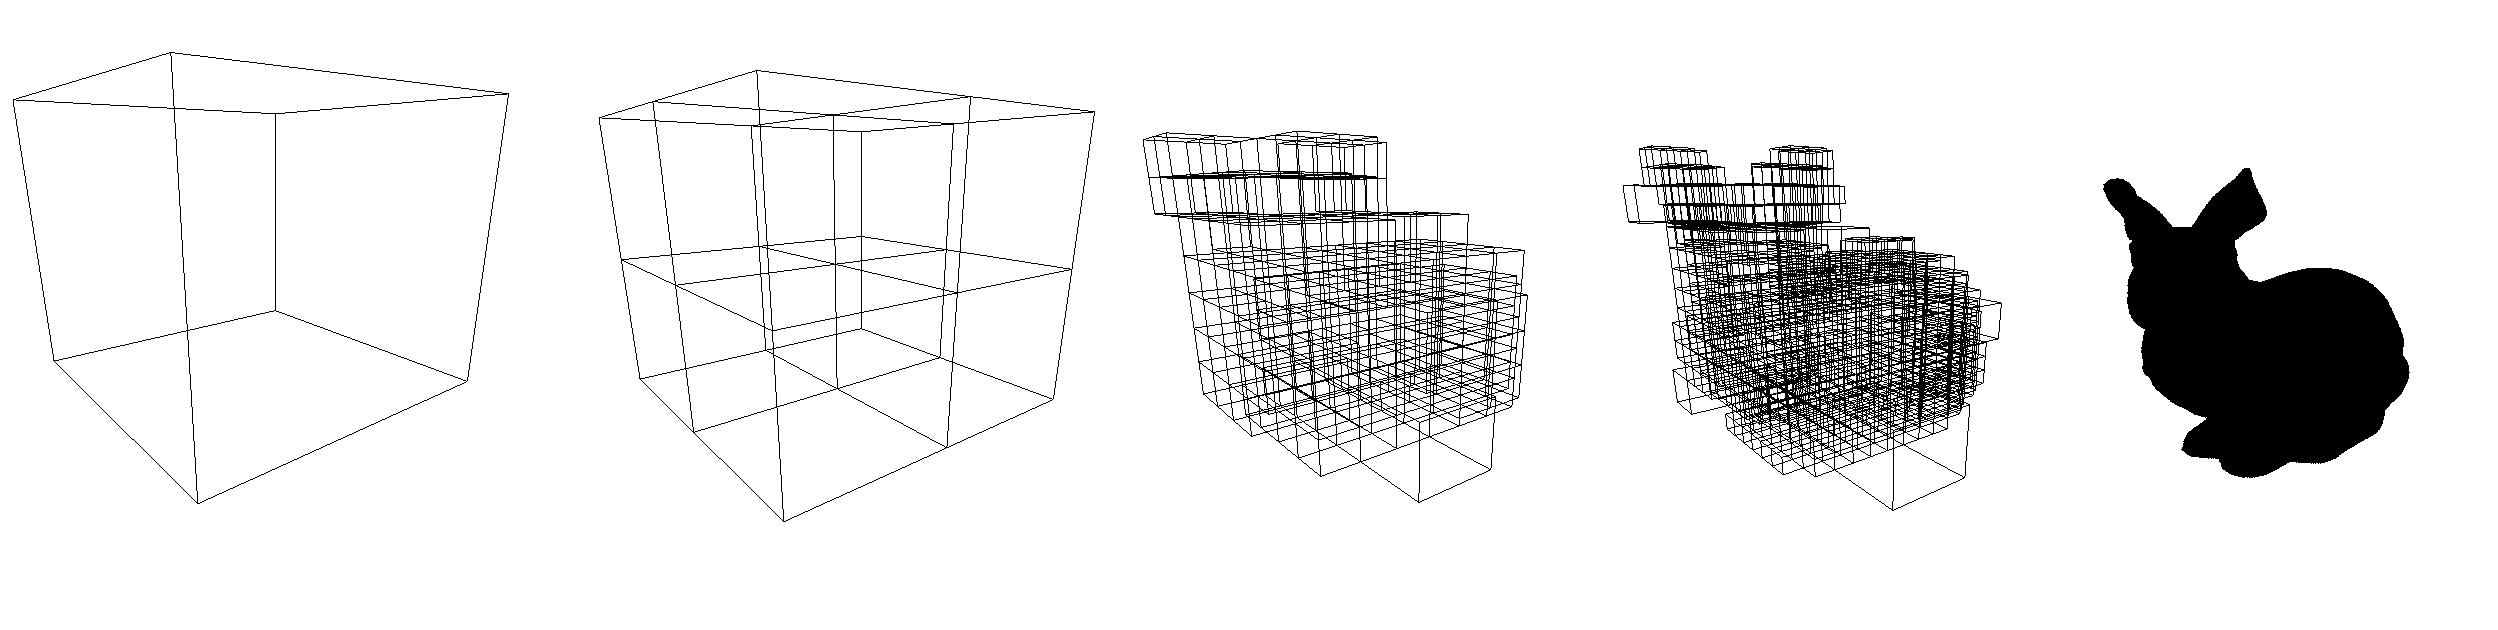
\includegraphics[width=16cm]{images/ch2/OctreeExample}
\caption{Visualization of OT Decomposition}
\label{OctreeExample}
\end{figure}


The goal of the OT and the QT is to store the size and attributes of each node implicitly. There are two main methods of representation, a packed traversal of the tree and a linear tree. The packed traversal method stores the hierarchy using a pre-defined traversal of the tree, and typically follows one of two orderings. These are, breadth-first traversal and depth-first traversal, these orderings are shown in figure \ref{TreeTraversalExample}. The depth-first traversal starts at the root, then works it's way down, top to bottom, then left to right of the tree. In essence, it travels to a node's children before considering its neighbours. In contrast, the breadth-first traversal goes to all nodes which are at the same depth before continuing on to lower levels. 

\begin{figure}[!h]
\centering
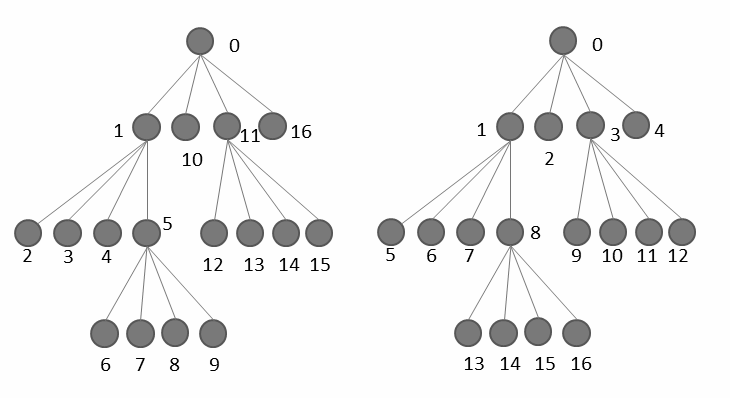
\includegraphics[width=12cm]{images/ch2/TreeTraversalExample}
\caption{Tree Traversals, Left: Depth First Traversal, Right Breadth First Traversal}
\label{TreeTraversalExample}
\end{figure}

Encoding these two tree traversal methods requires one nibble (4 bits) for a QT node, and one byte (8 bits) for an OT node, where the bits represent the structure of the sub-node. For example, the QT node bit sequence, $1001_2$ means that the node has two children (corresponding to the ones), the sequence $0000_2$ means the node is a leaf node. Each bit position indexes a child node using a pre-determined ordering. An example of a possible ordering for a quadrant and an octant is shown in figure \ref{ChildOrderExample}, both breadth-first and depth-first traversals use the same index method, the difference lies only in the order which nodes are visited. 

\begin{figure}[!h]
\centering
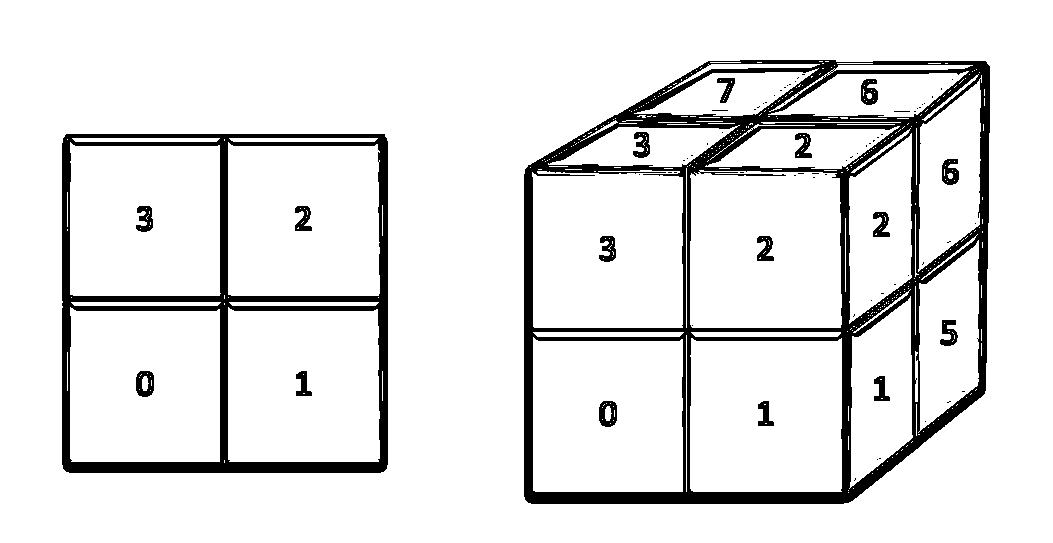
\includegraphics[width=12cm]{images/ch2/ChildOrderExample}
\caption{A possible child ordering for the QT (left), and the OT (right).}
\label{ChildOrderExample}
\end{figure}

The linear tree representation stores each leaf node individually. Each leaf is encoded as the pathway from the root to the leaf itself. This method was investigated in the 1980s \cite{Gargantini82Effective,Yufei88Octcodes}, but has not been used much in modern compression algorithms due to its inefficiency compared with the packed traversal method. An example of this structure is shown in figure \ref{LinearCellCodeRepresentation}, where each node: $a$, $b$, $c$, $\dots$ , $m$  is encoded as a variable length traversal path. The QT and OT are widely used in image \cite{Varma12Application} and 3D compression \cite{Schnabel06Octree}. Hanan Samet \cite{Samet88Fund1} presents an introduction to both of these structures, he also describes both tree storage methods in depth. 

\begin{figure}[!h]
\centering
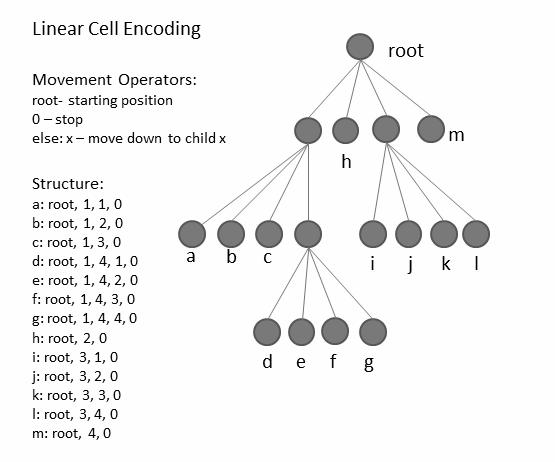
\includegraphics[width=12cm]{images/ch2/LinearCellCodeRepresentation}
\caption{A Linear Tree Code Representation Example}
\label{LinearCellCodeRepresentation}
\end{figure}



\section{3D Data Compression Schemes}







\section{Conclusion}

 % The Literature Review
\begin{savequote}[8cm]
  ``I have not failed. I've just found 10,000 ways that won't work.''
  \qauthor{Thomas Edison}
\end{savequote}
\makeatletter
\chapter{Methodology}

\section{Introduction}

Here we present several techniques used to extract dense 3D reconstruction from image/video data. In the first section we describe techniques in addition to Fourier volume registration. These include the recovery of translation, y-axis rotation and scale information as well as a technique for the recovery of a so called 7 degrees of freedom transform. \\

We also list notable speed-ups for volume registration which reduce the amount of processing by over a third. After this, a full 3D reconstruction technique based on the principles of phase correlation is presented. Then we also present two novel reconstruction data representations which may be used to efficiently represent and fuse 3D reconstructions. Lastly, different sensor inputs are discussed and some conclusions are given about the usefulness of this technique in the context of these sensors is presented.

\section{Fourier Volume Registration} 

\subsection{Recovery of Translation Values}

Given a volume $V_1$ and a spatially shifted version of it $V_2$, the offset along each axis, $(x,y,z)$ may be recovered if a suitable correlation between the two volumes can be found. \\

The measure of correlation between $V_1$ and $V_2$ can be found by shifting $V_1$ and $V_2$'s mean values to zero, then summing the element-wise multiplication of $V_1$ by $V_2$. Equation \ref{eqn:CorrelationEquation} computes this correlation measure.

\begin{equation} \label{eqn:CorrelationEquation}
\sum_{z=0}^{N}\sum_{y=0}^{N}\sum_{x=0}^{N}(V_1(x,y,z)-avg(V_1)) \times (V_2(x,y,z)-avg(V_2))
\end{equation}

Using this measurement, two volumes which are similar in signal shape (element-wise-value to location correspondence) will give a larger measure of correlation than two volumes with a differing signal shape. If the volumes are first normalized we can regard volume $x$ is more aligned with volume $y$ than with volume $z$ given $x$ correlated with $y$ gives a larger value than $x$ correlated with $z$. \\

Cross-correlation searches over a space of translation parameters and outputs the optimal translation to align two volumes. It is optimal in the sense of correlation measurement. This is used as a best guess in terms of the alignment of the two volumes. It can be thought of as the optimization of parameters $x,y,z$ in equation \ref{eqn:CrossCorrelationEquation}.

\begin{equation} \label{eqn:CrossCorrelationEquation}
CrossCorrelate(Transform(V_1, x,y,z), V_2)
\end{equation}

Since we typically do not know the range of translation values $x,y,z$ to optimize for, we take into account the range from $[0,N]$ where $N$ is the width/height/depth of the volume. This gives a complexity of $N^6$. This is too computationally complex for practical volume sizes. Therefore, we use the properties of the Fourier Transform to reduce computational complexity. \\
 
The 3D Fourier transform transforms a volume from the 3D spatial domain into the 3D frequency domain. The frequency domain is a complex valued volume made up of sinusoids where each value in the frequency domain represents the magnitude, phase and direction of a wave.  \\


WARNING: show picture of 3D volume fft\\

WARNING: show picture of 3D pc surface\\

Using the properties of the Frequency domain, we can efficiently recover the optimal alignment translation parameters using a function called $PhaseCorrelation$ (Eq. \ref{eqn:PC_basic}). This function takes two volumes as input and returns the best alignment translation between them in terms of maximizing correlation.
\begin{equation} \label{eqn:PC_basic}
(x, y, z) = PhaseCorrelation(V_x, V_y)
\end{equation}
The $PhaseCorrelation$ function first applies 3D FFTs to volumes, $V_1$ and $V_2$, converting them into the frequency domain, i.e. $F_{1_{x,y,z}} = FFT(V_1)$ and $F_{2_{x,y,z}} = FFT(V_2)$. Taking the normalised cross power spectrum using Eq. \ref{eqn:PHCOR_eq} based on these frequency domain volumes computes the frequency domain of a new volume called the phase correlation volume. \\


\begin{equation} \label{eqn:PHCOR_eq}
F_{3_{x,y,z}} = \frac{F_{1_{x,y,z}} \circ F_{2_{x,y,z}}^*}{ | F_{1_{x,y,z}} \circ F_{2_{x,y,z}}^* | }
\end{equation}

Here, $\circ$ is an element-wise multiplication and $|x|$ is the magnitude function. Taking the inverse FFT of the frequency domain of the phase correlation volume, $F_3$ gives the phase correlation volume itself, $V_3$ ($V_3 = FFT^{-1}(F_3)$). The location of the peak value in the phase correlation volume $V_3$, $(x_1, y_1, z_1)$ gives the shift between the $V_1$ and $V_2$. The phase correlation volume is typically noisy making the peak difficult to locate. Each in the phase correlation volume evaluates the correlation between $V_1$ (translated by the location of the peak) and $V_2$.


\subsection{Recovery of Y-Axis Rotation and Scale}

Using the phase correlation procedure along with some spatial transformation functions allows the computation of a single axis of rotation (out of 3) along with the scale difference between two volumes. If $V_1$ and $V_2$ are translated, rotated and scaled versions of the same volume, such that they are related by some translation $(t_x, t_y, t_z)$, y-axis rotation $\theta$, and scale $\varphi$.\\


WARNING: show picture of log-spherical transform\\

Here we describe how to compute the rotation and scale parameters, further action is required to recover translation. The first step, given two volumes $V_1$ and $V_2$ of size $N^3$ is to apply a Hanning windowing function (Eq. \ref{eqn:Hann}). This function assists in filtering the volumes prior to a discrete Fourier transform being applied to them. Since the discrete Fourier transform relies on a continuous signal (volume) and this cannot be used in the calculation, by reducing the signal strength near the volume borders, we can improve the accuracy of the discrete Fourier transform.
\begin{equation} \label{eqn:Hann}
\scriptstyle
HW_{x,y,z} = \frac{1}{2}\left(
1 - cos \left(
\frac{2\pi
\left(
\sqrt{\left(\frac{N}{2}\right)^3} -
\sqrt{
\left(x-\frac{N}{2}\right)^2 + \left(y-\frac{N}{2}\right)^2 + \left(z-\frac{N}{2}\right)^2
}
\right)
}
{2\sqrt{\left(\frac{N}{2}\right)^3} - 1}
\right)
\right)
\end{equation}
The rotation and scale factors can only be recovered if translation information is removed from the two volumes. Therefore we take the magnitude of the FFT of the volumes, $M_1 = |FFT(V_1)|$, $M_2 = |FFT(V_2)|$. Since the magnitude values do not contain phase information they do not, by nature, contain location information of the volume (translation information). The zero-frequency of both $M_1$ and $M_2$ is next shifted to the center of the volume and the log of the result is taken $M'_1 = Log(M_1)$, $M'_2 = Log(M_2)$. Like in phase correlation the log function spreads out the contribution of the frequencies so that high frequencies contribute as much as lower frequencies which have larger magnitudes. A log-spherical transform is then used to turn rotation and scaling into translation for both $M'_1$ and $M'_2$. Eq. \ref{eqn:Log_Spherical} shows the corresponding log-spherical space coordinate $(X_{log-spherical}, Y_{log-spherical}, Z_{log-spherical})$ for a given $(x,y,z)$ euclidean space coordinate.
\begin{equation} \label{eqn:Log_Spherical}
\begin{split}
X_{log-spherical} & = \frac{atan\left(
\left(\frac{x-\frac{N}{2}}{\sqrt{x^2+y^2+z^2}}\right)
\left(\frac{y-\frac{N}{2}}{\sqrt{x^2+y^2+z^2}}\right)^{-1}
\right)N}{360}\\
Y_{log-spherical} & = \frac{acos\left(
\frac{y}{\sqrt{x^2+y^2+z^2}}
\right)N}
{180} \\
Z_{log-spherical} & =\frac{log\left(\sqrt{x^2+y^2+z^2}\right)N}{log\left( \frac{N}{2.56} \right)} \\
\end{split}
\end{equation}
The log-spherical transforms of $M'_1$ and $M'_2$ are then phase correlated to find the shift between them, $(x_{M'},y_{M'},z_{M'}) = PhaseCorrelation(M'_1, M'_2)$. The rotation $\theta$ and scale $\varphi$ factors between $V_1$ and $V_2$ can then be found from the shift parameters using Eq. \ref{eqn:ROTATIONSCALEFROMXM} . 
\begin{equation} \label{eqn:ROTATIONSCALEFROMXM}
\begin{split}
\theta & = \frac{-360x_{M'}}{N}\\
\varphi & = e^{
-\left(
2.56^{-1}N
\right)z_{M'}N^{-1}
}
\end{split}
\end{equation}
Using $\theta$ and $\varphi$, $V_1$ can now be inverse transformed (using $(\frac{N}{2}, \frac{N}{2}, \frac{N}{2})$ as the origin). This aligns $V_1$ and $V_2$ with respect to scale and y-axis rotation. The translation parameters $(t_x, t_y, t_z)$ can then be found using phase correlation as given in Eq. \ref{eqn:FINALTRANS}.
\begin{equation} \label{eqn:FINALTRANS}
(t_x, t_y, t_z) = PhaseCorrelation(scale(rotate(V_1,\theta),\varphi), V_2)
\end{equation}
The complete function to recover translation, rotation and scaling, combining equations \ref{eqn:PHCOR_eq}-\ref{eqn:FINALTRANS} as is denoted in \ref{algorithm:PCSLAM} is \ref{eqn:FULLPC}.
\begin{equation} \label{eqn:FULLPC}
(\theta, \varphi, t_x, t_y, t_z) = PhaseCorrelation_{\theta \varphi t_x t_y t_z}(V_m, V_n)
\end{equation}

\subsection{Full Recovery of 3D Rotation}

\label{FullRecovery3DSection}

In order to recover full 3D rotation (as well as scale and translation) the model must first be aligned by some common axis. PCA or Principals Component Analysis is a well known technique for recovering the primary axes of an N-dimensional signal. In this case, we can use the most accurate axis (the eigen-vector with the largest corresponding eigen-value) to align two volumes, then y-axis rotation, scale and translation values can be recovered by the described FFT based volume registration method. \\

WARNING: SHOW picture of this PCA procedure

PCA is a capable registration technique on its own, but when faced with non-overlapping, missing or noisy data it typically fails on its own. The technique of alignment is discussed in the following sections. \\

Given a 3-dimensional signal $A$ of length $N$, the co-variance of the signals between two of the dimensions ($x$ and $y$) is given as a function in equation \ref{eqn:Covariance3DSignal}.

\begin{equation} \label{eqn:Covariance3DSignal}
Cov(A_x,A_y) = \sum_{i=0}^{N}(A_{x_i} - A_{x_{mean}})(A_{y_i} - A_{y_{mean}})
\end{equation}

Here, $A_{x_{mean}}$ and $A_{y_{mean}}$ are the mean values of these x and y dimensions of $A$. 

Using the voxel locations of volume $A$ we can generate the covariance matrix \ref{eqn:CovarMatrix}. This matrix describes the how each coordinate changes with respect to each other.

\begin{equation} \label{eqn:CovarMatrix}
\left[
\begin{array}{ccc}
Cov(A_x, B_x) & Cov(A_x, A_y) & Cov(A_x, A_z) \\
Cov(A_y, B_x) & Cov(A_y, A_y) & Cov(A_y, A_z) \\
Cov(A_z, B_x) & Cov(A_z, A_y) & Cov(A_z, A_z) \\
\end{array}
\right]
\end{equation}

The 3 eigen-vectors of the covariance matrix describe the primary axis of the signal $A$ and the 3 corresponding eigen-values describe the strength of these axes. The eigen-vector/axis with the largest corresponding eigen-value is the principal component. The principal component is used to align data to a common axis. Here we define the principal axis (component) of a 3D signal $A$ as $A_{pa}$. \\

Given a 3D volume $V$, with a computed principal axis $V_{pa}$ and mean $V_{mean_location}$, we can construct a matrix to normalize the 3D data in terms of the principal axis.

Given $V_{pa}$ a vector pointing along the principal axis of $V$, we compute the forward vector as 


\begin{equation} \label{eqn:fwdVector}
Fwd = \left(\left[
\begin{array}{c}
V_{pa_{x}}\\
V_{pa_{y}}\\
V_{pa_{z}}\\
\end{array}
\right] \times \left(\left[
\begin{array}{c}
1\\
0\\
0\\
\end{array}
\right] \times \left[
\begin{array}{c}
V_{pa_{x}}\\
V_{pa_{y}}\\
V_{pa_{z}}\\
\end{array}
\right]\right)\right) \times \left[
\begin{array}{c}
V_{pa_{x}}\\
V_{pa_{y}}\\
V_{pa_{z}}\\
\end{array}
\right]
\end{equation}

Here, $\times$ is the cross-product of the vectors. The right pointing vector is computed as orthogonal to the forward vector and the common vertical axis $V_{pa}$,


\begin{equation} \label{eqn:fwdVector}
Rgt = \left[
\begin{array}{c}
V_{pa_{x}}\\
V_{pa_{y}}\\
V_{pa_{z}}\\
\end{array}
\right] \times \left[
\begin{array}{c}
Fwd_x\\
Fwd_y\\
Fwd_z\\
\end{array}
\right]
\end{equation}

Then the volume can be normalized to an axis based on the input data. This is done using a matrix which transforms the data to the origin, then corrects the vector $V_{pa}$ to be the new up axis, then transforms back. The matrix in equation \ref{eqn:CorrectUpMat} computes this,


\begin{equation} \label{eqn:CorrectUpMat}
CorrectMat(V) = \left[
\begin{array}{cccc}
1 & 0 & 0 & V_{mean_x} \\
0 & 1 & 0 & V_{mean_y} \\
0 & 0 & 1 & V_{mean_z} \\
0 & 0 & 0 & 1 \\
\end{array}
\right] \left[
\begin{array}{cccc}
Rgt_x & Rgt_y & Rgt_z & 0 \\
V_{pa_x} & V_{pa_y} & V_{pa_z} & 0 \\
Fwd_x & Fwd_y & Fwd_z & 0 \\
0 & 0 & 0 & 1 \\
\end{array}
\right] \left[
\begin{array}{cccc}
1 & 0 & 0 & -V_{mean_x} \\
0 & 1 & 0 & -V_{mean_y} \\
0 & 0 & 1 & -V_{mean_z} \\
0 & 0 & 0 & 1 \\
\end{array}
\right]
\end{equation}


To recover a matrix for full 3D rotation, scale and translation for given volumes $Volume_A$ and $Volume_B$, we first compute the correction matrices using PCA and the technique described above for both $Volume_A$ and $Volume_B$ as $C_A = CorrectMat(Volume_A)$ and $C_B = CorrectMat(Volume_B)$. The transformation matrix relating $Transform(Volume_A, C_A)$ and $Transform(Volume_B, C_B)$ is computed as $RST$. The final transform then relating $Volume_A$ to $Volume_B$ is computed as,

\begin{equation} \label{eqn:FullRSTTransform}
R_{x,y,z}ST Matrix = C_{B}^{-1} \times RST \times C_A
\end{equation}

This technique is capable of extending Fourier registration to take into account full 3D rotation. The technique simply requires a single iteration over the data to compute the principal components then a rotation-scale-translation phase correlation technique is used to compute the scale, translation and y-axis rotation. 

WARNING: show an example of this working

\subsection{Filtering Techniques}

\subsection{Fast Fourier Volume Registration}

3D phase correlation is CPU and GPU intensive, so in order to reduce complexity we tried to minimize processing in areas which require the most computation time. In out Fourier based volume registration method defined in the previous section, this occurs in the two 3D phase correlations which need to be computed. We describe the method of reduction here; a block diagram for this technique is given in figure \ref{fig:PIPELINE3} WARNING:Given a picture for the sped up version too!. We refer to this method as fast volume registration (FVR) in reference to general volume registration (VR). The speedup begins by computing the 3D DFT of both input volumes and taking the magnitude of these. Rather than directly performing a 3D log-spherical transform and a 3D phase correlation operation on these volumes, we use a novel transform we call a spherical-map transform (details in \ref{SMTransform}).\\

\begin{figure*}[t]
\centering
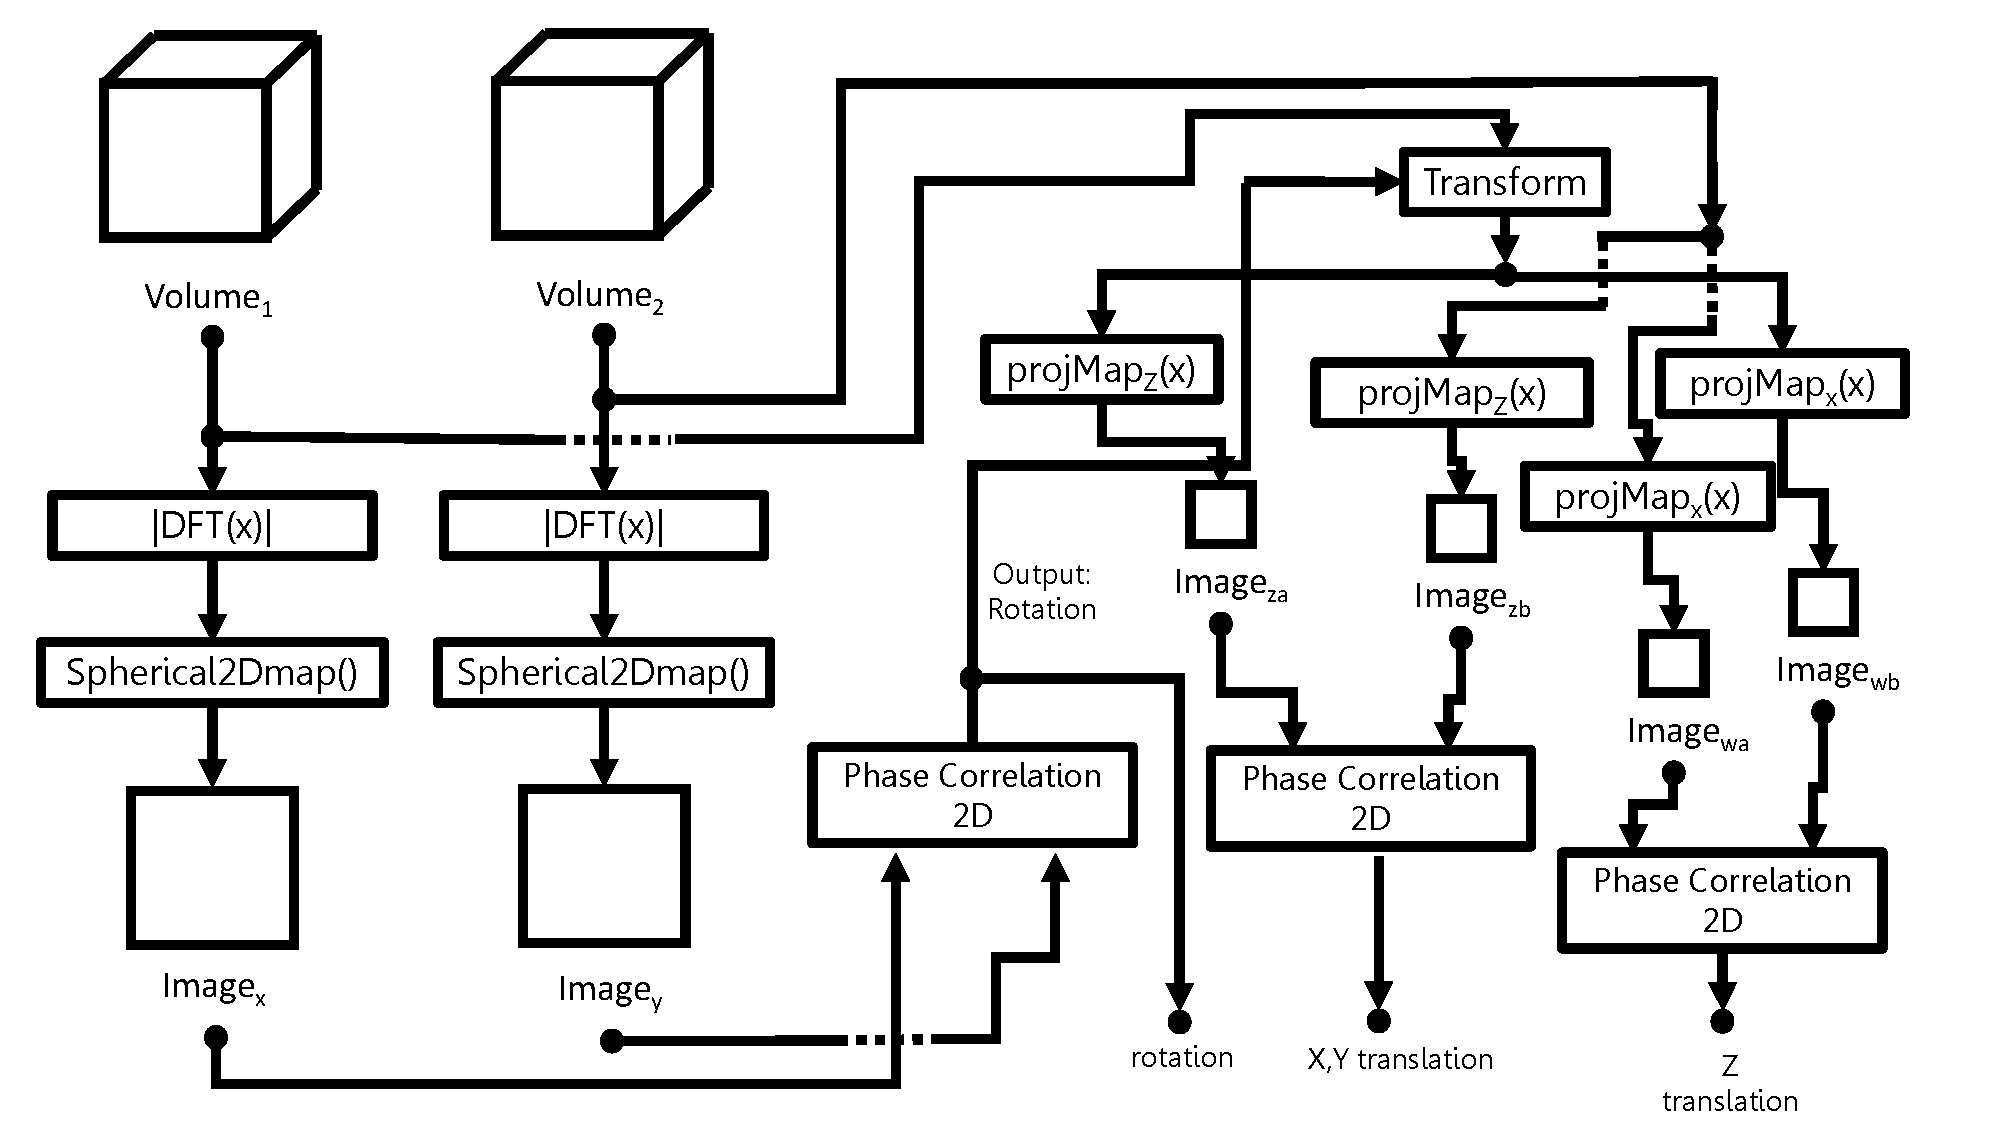
\includegraphics[width=6.0in]{images/ch2/pipeline3}
\caption{System Diagram for Fast Volume Registration}
\label{fig:PIPELINE3}
\end{figure*}

This transform converts rotation into translation whilst simultaneously unfolding the 3D space down to 2-dimensions. After this, a 2D phase correlation that requires significantly less processing compared with the 3D counterpart is used to compute the rotation. Next, having obtained the rotation parameter, the rotation is eliminated from the transformation by rotating the first volume by this parameter. The two volumes are then passed through two orthogonal projection mapping functions. This also converts the volumes to 2D space. We use two transforms for both volumes, one projection along the x-axis, another along the z-axis. Once the x-axis projections of both volumes are complete, we can do another 2D phase correlation to give us the z-translation. The 2D phase correlation of the z-axis projections gives us the x and y axis translations separating the original volumes. The final output of this method gives the rotation and translational shifts between the input volumes. The projections add little complexity to the overall algorithm and since 2D phase correlation operations are used in place of 3D ones, much computation time is reduced.

\subsection{Spherical-map transform}
\label{SMTransform}
The spherical map transform both reduces the 3D volume to a 2D image, and any rotation about the y-axis becomes x-axis translation in the output image. An example of the bunny model and the spherical-map transform of this model is given in figure \ref{fig:smtExample}, the mathematics are defined in equations \ref{eqn:invLPFuncs} and \ref{eqn:smtUpdate}. Given a coordinate in 2D Cartesian space x,y, we compute the ray $[Ray_x Ray_y Ray_z]^T$ from the volume center and sum up the voxel values along the ray (equation \ref{eqn:smtUpdate}). \\


\begin{equation} \label{eqn:invLPFuncs}
\begin{split}
Ray_x(x,y) & = cos\left(\frac{360x}{N}\right)sin\left(\frac{180y}{N}\right)  + \frac{N}{2} \\
Ray_y(y) & = cos\left(\frac{180y}{N}\right) + \frac{N}{2} \\
Ray_z(x,y) & = 	sin\left(\frac{360x}{N}\right)sin\left(\frac{180y}{N}\right) + \frac{N}{2}
\end{split}
\end{equation}

\begin{equation} \label{eqn:smtUpdate}
Im_{x,y} = \sum_{r=1}^{(2^{-1}N)^{1.5}}{Vol(Ray_x(x,y)r, Ray_y(y)r, Ray_z(x,y)r)} 
\end{equation}

This process essentially sums up the values along a given ray defined by scaling spherical coordinates and adding up the values intersecting the ray. The resulting image, maps 3D y-axis rotation to 2D x-axis translation.  \\

\begin{figure*}[t] 
        \centering
        \begin{subfigure}[b]{4.2in}
                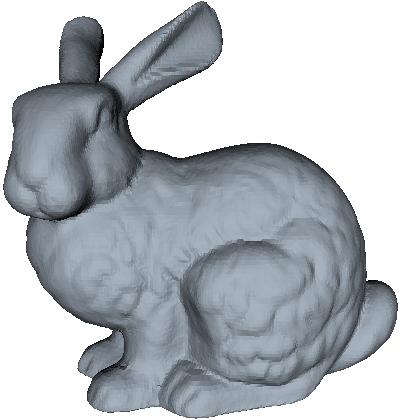
\includegraphics[width=4.2in]{images/ch2/bunny}
                \caption{original}
                \label{fig:bunnyOrig}
        \end{subfigure}
        \begin{subfigure}[b]{4.2in}
                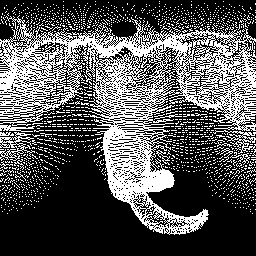
\includegraphics[width=4.2in]{images/ch2/spherical2DMap}
                \caption{transform}
                \label{fig:bunnySPTed}
        \end{subfigure}%
        \caption{The Spherical Map Transform.}
       \label{fig:smtExample}
\end{figure*}


\subsection{Projection-map transform}

The projection map transform is similar to an orthogonal projection of the volume along some given axis. For the projection map transform, given an output image $Im_a$ and an input volume $Vol_a$, each pixel in $Im_a$ is defined mathematically as the summation of values along a particular axis given the image coordinates. The x-axis transform and the z-axis transform are defined in equations \ref{eqn:xPMT} and \ref{eqn:zPMT} respectively. \\

WARNING: add in a picture here

\begin{equation} \label{eqn:xPMT}
Im(z,y) = \sum_{x=0}^{N}{Vol_a(x,y,z)}
\end{equation}

\begin{equation} \label{eqn:zPMT}
Im(x,y) = \sum_{z=0}^{N}{Vol_a(x,y,z)}
\end{equation}

The process defined by equation \ref{eqn:xPMT} maps 3D z-axis translation to 2D x-axis translation, whilst equation \ref{eqn:zPMT} maps 3D x-axis and y-axis translation into 2D x-axis and y-axis translation.


To assess the performance of our method, the size of the volumes being registered is defined as $N^3$ whilst each frame is sampled at a resolution of $W$ $\times$ $H$. The projection process requires $12WH$ operations whilst re-sampling the point cloud requires $2WH$ operations. The Volume Registration process, $VolumeRegister{\theta \varphi t_x t_y t_z}(V_1, V_2)$ consists of 2 $\times$ Hanning windowing processes, 2 $\times$ 3D FFTs, 2 $\times$ volume-logs, 2 $\times$ log-spherical transforms, 2 $\times$ phase correlation processes and 1 $\times$ linear transformation and peak finding. 

The Hanning windowing function requires 26 operations. The 3D FFT has complexity of $3N^3\log{N}$, the log and log-spherical transform functions require 3 and 58 operations per voxel respectively. Multiplying two frequency spectra together and transforming a volume requires 15 and 30 operations per voxel respectively. Finding the peak value requires $2N^3$ operations. The complexity in terms of number of operations for the phase correlation process is given in Eq. \ref{eqn:PCFULLPERFORMANCE} This process requires 2 $\times$ 3D FFTs, 1 $\times$ frequency spectra multiplication, and 1 $\times$ peak finding operation. 
\begin{equation} \label{eqn:PCFULLPERFORMANCE}
6N^3\log{N} + 2N^3 + 15
\end{equation}
The total complexity can then be found by taking into account the projection and re-sampling totals as well as the total for $VolumeRegister{\theta \varphi t_x t_y t_z}(V_1, V_2)$. Tallying the number of operations for each process and multiplying them by number of times the process is performed gives us the number of operations as a function of $W$, $H$ and $N$ in Eq. \ref{eqn:FULLPERFORMANCE}.
\begin{equation} \label{eqn:FULLPERFORMANCE}
6N^3 + 28WH + 18(N^3\log{N}) + 230
\end{equation}



To compare performance of the generic volume registration method with the speed up, we use the complexity defined in equation \ref{eqn:FULLPERFORMANCE}. Here, we ignore the cost of projecting the depth map. The 3D DFT has complexity $3N^3log(N)$. This is the first step (see figure \ref{fig:PIPELINE3}), the next is the spherical-map transform which is complexity $45N^3$. If processed on the GPU the performance becomes 45 operations per voxel assuming that one voxel is assigned to one unit of processing. A 3D transform is 30 operations per voxel, 2D phase correlation requires 15 operations to multiply the frequency spectra and $2N^2log(N)$ operations to do the 2D FFT. Finally a projection map transform requires 1 operation per voxel. \\

In total, the proposed method requires $2 \times$ 3D FFTs, $2 \times$ spherical-map transforms, $1 \times$ 3D geometrical transformation, $3 \times$ 2D phase correlations and $4 \times$ projection map transforms. The total complexity is added up for all of these functions and given in equation \ref{eqn:FULLPERF2}. \\

\begin{equation} \label{eqn:FULLPERF2}
6log(N)\times (N^3 + N^2) + 169
\end{equation}

Figure \ref{fig:perfComp} provides a visualization of the performance improvement which the proposed method achieves over the original Fourier volume registration approach. It is clear that the proposed method is around 3 times faster
than the original Fourier based volume registration approach. This is due to the reduction in the amount of data to process afforded by the novel spherical-map transform and orthogonal projection methods.

\begin{figure}[t]
\centering
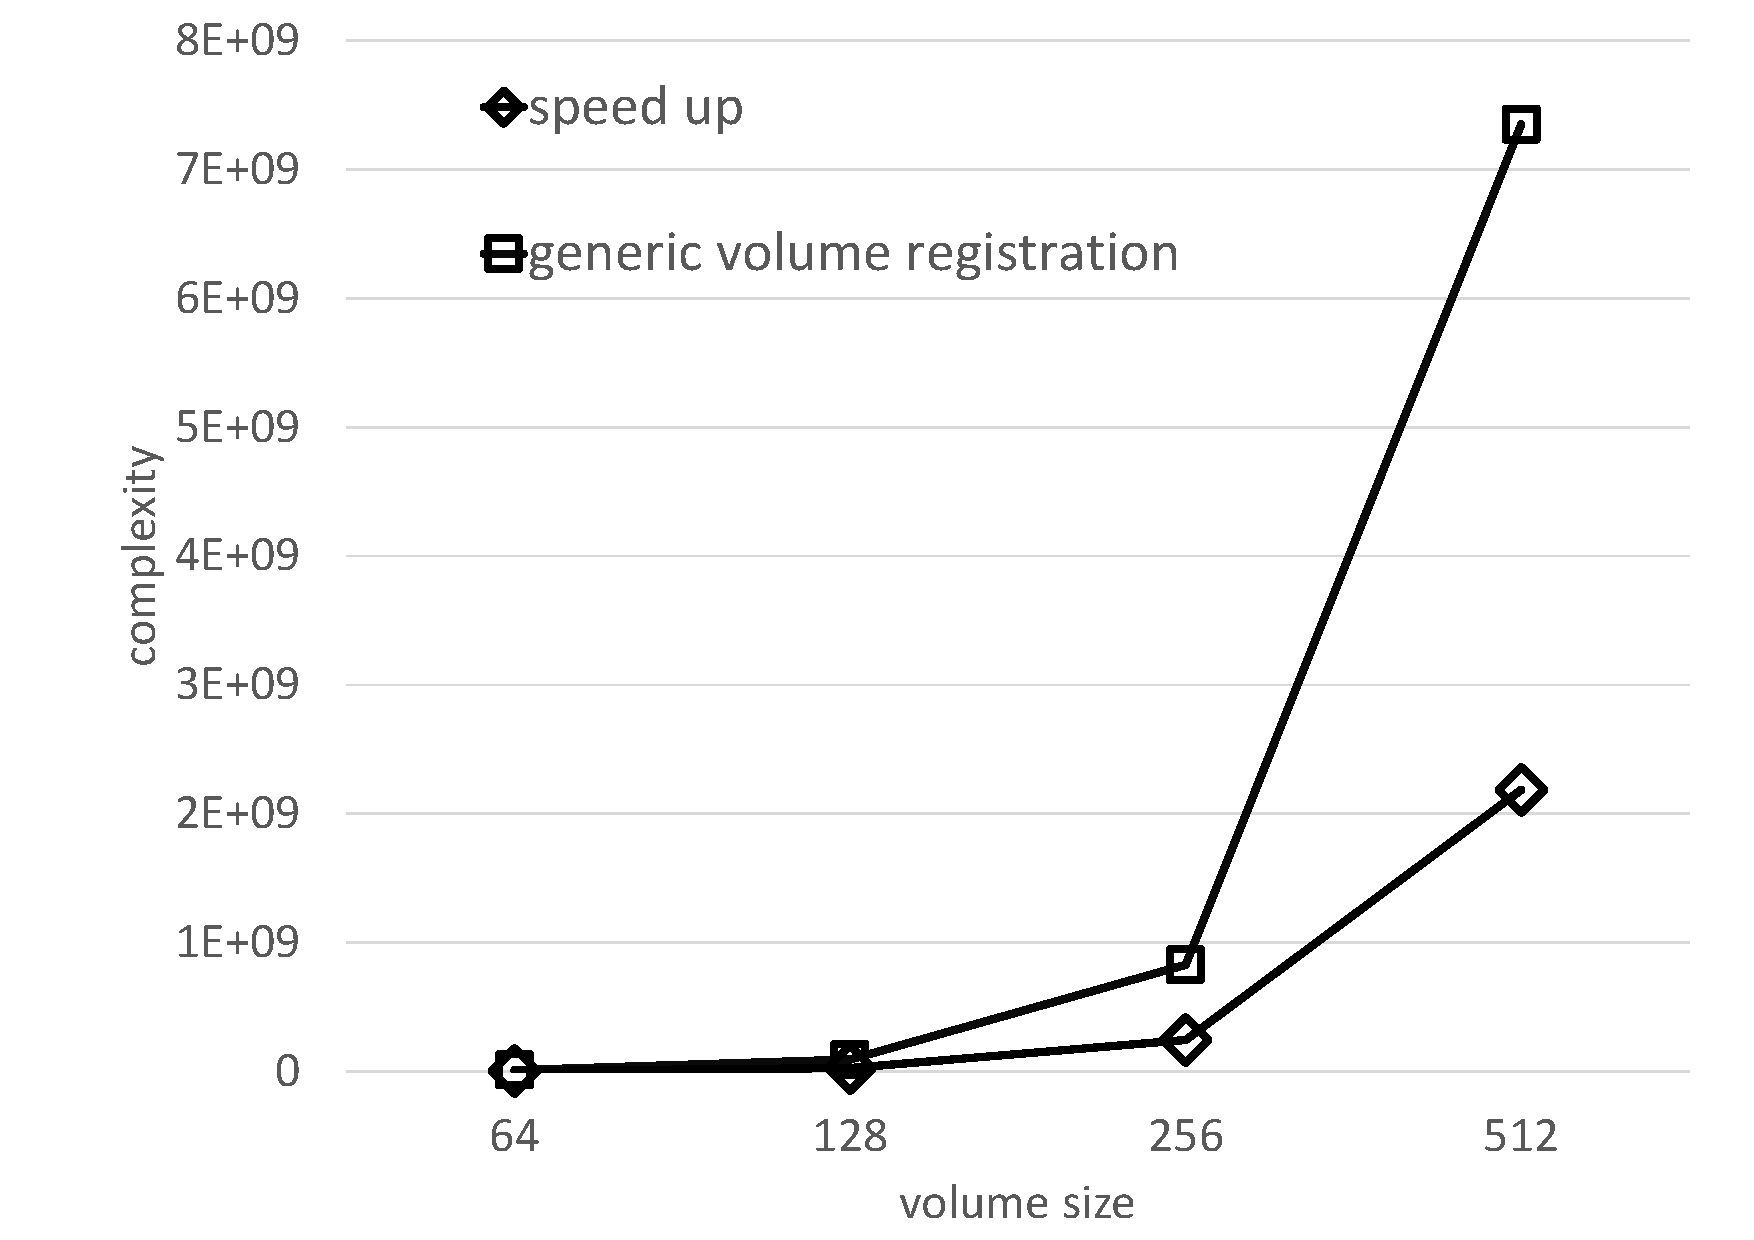
\includegraphics[width=4.0in]{images/ch2/perfcomp}
\caption{Comparison of performance between volume registration and the proposed speed up for different volume sizes.}
\label{fig:perfComp}
\end{figure}



\section{Fourier Volume Registration based 3D Reconstruction}


In this section we describe the general technique of recovering pose estimation via Fourier volume registration techniques. Several methods may be used and each has its own advantages and disadvantages and suitability depends on pose restriction, camera accuracy, noise levels and input data. 


\subsection{A Volume Registration based 3D Reconstruction Pipeline}

\label{METHOD_SECLL}
The proposed 3D reconstruction method consists of various steps. First each frame $f_i$ that is captured, consisting of a colour and depth image pair is projected into 3D space, forming colour point cloud $points_i$ and re-sampled into a volume $V_i$. Then, the transform parameters between pairs of volumes $V_i$ and $V_{i+1}$ are estimated using $VolumeRegister_{\theta \varphi t_x t_y t_z}$ shortened to $VR_{\theta \varphi t_x t_y t_z}$. These parameters are used to update transformation matrix $M$. The points corresponding to $f_2$ ($points_1$) are then transformed using the updated $M$ matrix and added to the cumulative $PointCloud$ database. Two lists, $Cameras$ and $Poses$, are also updated to track camera pose and location per frame. This basic procedure is given in listings \ref{algorithm:PCSLAM} and elaborated upon in subsequent subsections.
\begin{figure}
\begin{lstlisting}[language=c++,caption=Phase Correlation Based SLAM Algorithm,label=algorithm:PCSLAM,mathescape,basicstyle=\ttfamily]
$f_1$ = ReadFrame();
$PointCloud$ = project($f_1$);
$M$ = IdentityMatrix();
$Camera$ = $[0, 0, 0]^T$;
$Pose$ = $[0, 0, 1]^T$;
$Cameras$ = $\left[Camera\right]$, $Poses$ = $\left[Pose\right]$;
while(more frames){
	$f_2$ = ReadFrame();
	$points_1$ = project($f_2$);
	$points_2$ = project($f_1$);
	$V_1$ = ResampleVolume($points_1$);
	$V_2$ = ResampleVolume($points_2$);
	$(\theta, \varphi, t_x, t_y, t_z) = VR_{\theta \varphi t_x t_y t_z}(V_1, V_2)$;
	$M = M \times$TransformMat($(\theta, \varphi, t_x, t_y, t_z)$);
	$points_1$ = Transform($points_1$, $M$);
	$PointCloud$ = $PointCloud \cup points_1$;
	$Camera$ = $M^{-1} \times Camera$;
	$Pose$ = $M^{-1} \times Pose$;
	$Cameras.add(Camera)$;
	$Poses.add\left(\frac{Pose-Camera}{|Pose-Camera|}\right)$;
	$f_1$ = $f_2$;
}
\end{lstlisting}
\end{figure}


The input to our method is a color and depth image pair, $f(u,v)$ and $g(u,v)$ obtained using an Asus Xtion PRO LIVE sensor at a resolution of $640 \times 480$. Each pixel is projected into 3D space using $X_{u,v} = \frac{(u - c_x)Z_{u,v}}{f}$, $Y_{u,v} = \frac{(v - c_y)Z_{u,v}}{f}$ and $Z_{u,v}$ = $g(u,v)$. 
Here, $[c_x c_y]^T$ represent the center of the image whilst $f$ represents the focal length, defined as $525.0$. The point clouds generated by projecting these images are then quantized into image volumes. Results reported in this paper were obtained using volumes of $384^3$ voxels in size.

\begin{figure*}[t]
\centering
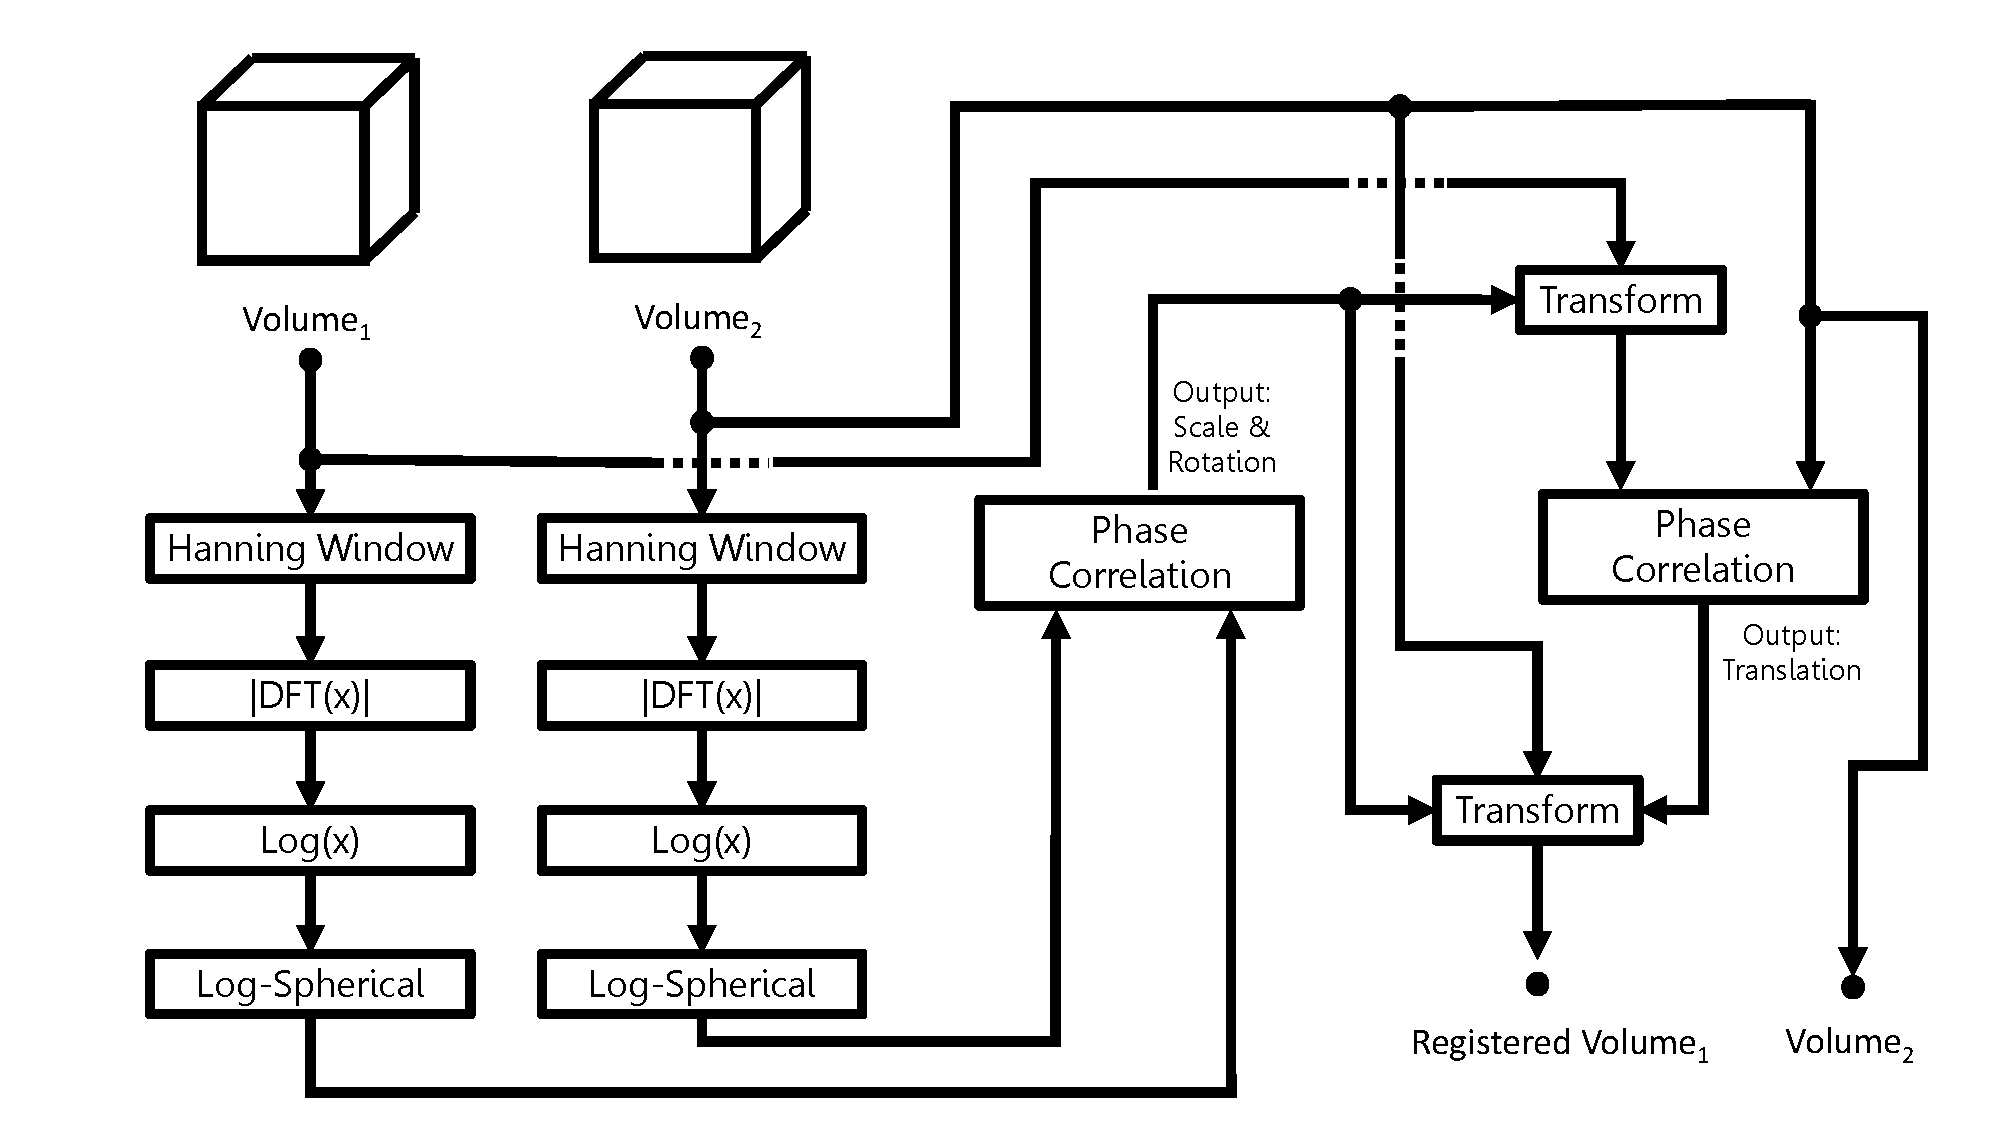
\includegraphics[width=6.0in]{images/ch2/pipeline2}
\caption{System Diagram for Registration Process}
\label{fig:PIPELINE}
\end{figure*}


\subsection{Error metrics}

In order to evaluate the accuracy of volume registration we use several error metrics including: Hausdorff error, mean squared error and the percentage of matched voxels. We describe mathematically those techniques here. All measurements are based on a simple function which computes the nearest neighbour for a given 3D point or voxel given a volume (or collection of 3D points). We define such a function, named nearest-neighbour in equation \ref{eqn:NN}.

\begin{equation} \label{eqn:NN}
NN(p, V) =  \{ q \in V | (Dist(q, p) < Dist(k, p))  \forall k \in V \}
\end{equation}

This function retrieves the closest corresponding point given a query point $p$ and a volume or point cloud of points, $V$. This function can be used to provide omni-directional error functions based on Hausdorff, mean squared and percentage accuracy error metrics.

Here some one-way error functions are described. The one was Hausdorff error is defined in \ref{eqn:HDOW} 

\begin{equation} \label{eqn:HDOW}
\sum_{k=0}^{N} Dist(P_k, NN(P_k, Q))
\end{equation}

\subsection{Reconstruction Integration}

Using the techniques of registration described in the above sections, there are several techniques which may be used to integrate these registered data. In most experiments we use the volume integration to combine the registered data in a single global model. We also propose several techniques for data representation and evaluate their abilities (see section \ref{sec:3DDataRepresentations}). As for the typical volume integration used, we create volumes with dimensions of $512\times 512\times 512$, although larger sizes may be used for increased accuracy. Once a frame is registered, it is projected into the volume. \\

This projection follows the following formula


\begin{equation} \label{eqn:volIntegration}
\begin{split}
x^{1} & = floor((x - frameCenter_x) \times scalar + volumeCenter_x) \\
y^{1} & = floor((y - frameCenter_y) \times scalar + volumeCenter_y) \\
z^{1} & = floor((z - frameCenter_z) \times scalar + volumeCenter_z)
\end{split}
\end{equation}

$frameCenter$ is the center of the projected frame space and $volumeCenter$ is the center of the integration volume, typically scalar is set to 1 or is used to trade-off resolution and map size. An example of an integration process is illustrated in figure XFDF. 


\subsection{Advantages and Disadvantages}





\section{3D Reconstruction Data Representation}
\label{sec:3DDataRepresentations}
In this section we introduce two data representations for recording 3D reconstructions. These novel representations are based on the Octree method. The representations are both designed to compress the data. These methods are inspired by the Shade-Tree and Interpolated Leaf Quad-Tree representations \cite{Gonzalez07ShadeTree, Lincoln13Interpolating} which are used for image compression. These techniques make use of Quad-Tree decomposition and have been shown to outperform several transform based methods of compression. 

\subsection{Octree Decomposition}

In this section we explain Octree decomposition. This strategy forms a cube shaped space around some 3D volumetric data. A data representation is then computed using the location and size of the cube. A measurement system is used to decide if the current data representation fits the data within the cube well or not. If so, then the data representation is used instead of the data. If not, the cube is broken down into 8 sub-cubes and the process is repeated. At each level of decomposition, the data representation achieves finer detail, but more nodes must be stored which means less compression. An example of the Octree is illustrated in figure [INSERT IT HERE].


\subsection{3D ShadeTree Coding}

The Shade-Tree compression system CITE HERE, was designed for the compression of 2D image data. However, this method is easily extended to 3D Volumetric data. In this system, octants are decomposed in the same manner as with a regular octree but the leaf node representation is different. In the Shade-Tree, the corner values in the volume are sampled for each node. Figure XXXXFFG shows an example of these corners given an Octree. The corner values are stored instead of the data within the cube. \\


The actual data representation is formed by interpolating between these 4 corner values to generate the data within the node. This representation saves space by storing 4 corner values only rather than the dense volumetric data. The method also boasts the ability for nodes to share data. For example, if two leaf nodes happen to share a corner we can simply encode the corner once using another data structure at the decompression stage at no cost to the representation. This is illustrated in figure FEFEEF. \\

This data representation may also be used to represent Signed Distance Functions, which are now commonly used in 3d reconstruction as a means of representation. In fact, such a scheme would greatly benefit the compression method of the Shade-Tree since its data is typically represented as smooth changes along a given path. 

\subsection{PlaneTree Coding}

Our method is based on octree subdivision, it begins by placing the mesh within a cube. It checks whether the the representation corresponding to this single cube is at a desired level of quality. If it is not, the cube is decomposed into 8 sub-cubes. For each sub-cube associated with the mesh, the process repeats. This process is typically controlled using an error threshold and a maximum depth value. At each level of subdivision, the error between the sub-cube (or node) representation of the space is compared to the part of the model within the cube. If the error is below the error threshold, decomposition stops. Likewise, if the level of subdivision is greater or equal to the maximum depth value, decomposition also stops. \\

In the typical octree node representation, the raw cube is used to represent the space. Unless this cube is small (deep within the tree) the error is typically high. Trees which are very deep require more storage space. Our method stores arbitrary first order planes within nodes at 20 bits per leaf. This small bit cost per leaf node greatly improves compression performance compared to the octree and makes it competitive with state of the art methods. \\

 
In the following sections, we present the details of the Plane-Tree in terms of subdivision, leaf node plane computation and representation as well as compression and decompression.


\subsection{Octree Subdivision}

Prior to compression, the input 3D model is normalized into a $512^3$ space. Starting with the cube which represents this space, we compute our 3D plane representation. Then the mean squared error between the sampled points of the plane and the sampled points of the model (which lie within the cube) is computed. If this value is below a given threshold, or the maximum level of subdivision is reached, decomposition stops. Alternatively if both of these predicates are not met, the cube is divided into 8 sub-cubes. Each sub-cube is then tested to see whether part of the mesh lies within it. If so, the process it repeated for that cube, otherwise no action is taken. \\

Each cube/sub-cube is referred to as a node. Each node which has no children is referred to as a leaf node. During compression/decompression, our plane based representation is only stored at leaf nodes, with non-leaf nodes serving only as paths giving the location of leaf nodes. Below, the computation and representation of our novel leaf node representation is discussed. \\

\subsection{Leaf Node Computation and Representation}
\label{NRep}
Our novel leaf node representation better represents the mesh which intersects it compared to the octree, it does so by using a first order plane. This representation requires only 20 bits, allowing us to achieve higher quality models whilst saving on bits which would otherwise be used to form a deeper, and thus more costly octree representation. It also gives our method an advantage at low bitrates. \\

In order to generate a plane for a given leaf node, we first sample the mesh within the node space. Using these points, the x, y and z axis variances are measured. These indicate how much variation lies across each axis within the node. We then find the plane using least squares, solving for the axis with the lowest variance. Once we have coefficients describing the plane, we use a single point on the plane, and the plane normal to describe it. \\

Using a point on the plane and a plane normal, we can find a set of triangles which represent the plane within the node. We first find all points in which the cube's edges intersect with the computed plane. Using the average point as the origin, and the plane's normal as the y-axis, we order the points based on their x/z angle. This gives us an ordered set of points which corresponds to a polygon defining the plane within the node. This polygon is then triangulated forming the final representation. This process is used at both the compression and decompression stages. \\

The triangles representing the plane within the node are then sampled along with the parts of the mesh lying within the node. The mean squared error (mse) is then taken between these samples for comparison with the error threshold value. Within the summation for the mse we use the closest point within the second point set, this is shown in equation \ref{eqn:MSE_1}.

\begin{equation}
 \label{eqn:MSE_1}
MSE(pts_1, pts_2) = \frac{1}{N}\sum_{i=0}^{N} (pts_{1_i} - closest(pts_{1_i}, pts_2))^2
\end{equation}

Using this equation and the sampled points from the plane triangles $p$, and the sampled points from the mesh $m$ (which lie within the cube), we take the average of both mean squared errors as a measurement of total error, $error = \frac{1}{2}MSE(p,m) + \frac{1}{2}MSE(m,p)$. This is the value which is compared with the error threshold to decide whether decomposition should stop or not. \\

In order to compress the data for our leaf node representation, we store the the plane using its normal vector and a single point lying on the plane. We store the normal vector using 12 bits (4 bits per coordinate). The point which lies on the plane is represented using two pieces of information, an edge number and a distance variable. First it must be mentioned that for a given plane which intersects a cube, a minimum of 3 of the cube's edges pass through the plane. We therefore record one of these edges (the edge number) and the distance from on of its end points (the distance variable). Each edge has a predefined number which identifies it, all edges also have a predefined start and end point. \\

Each cube has 12 edges in total, so 4 bits are used for the edge number, another 4 are used for the distance variable. Adding these to the normal vector totals to 20 bits per leaf node representation.  \\


\subsection{Compression and Decompression}

In order to compress our data structure we iterate through the tree in depth first order. If we encounter a non-leaf node, we first store a single bit of $1_2$. Then the configuration of the sub-nodes (since not every sub-node intersects the object) is stored as a single byte. Each bit is labelled $1_2$ if a particular sub-node exists and $0_2$ if it does not. This is possible since we order our sub-nodes in a predefined order. If a leaf node is encountered, we store a $0_2$, then record our 20 bit leaf node representation in three other files. One for the normal data, the distance variables and edge numbers totalling 4 files (tree, normals, distances and edge numbers). After the entire structure is stored we employ entropy encoding on each of these files. \\

In order to decompress our structure, we read the first bit of the output file. This checks if the current node is a leaf or not. If it is, we read out a 20 bit plane representation (from the three separate files) and generate a list of triangles representing where the plane intersects the node (explained in section \ref{NRep}). These triangles are then added to a final database which represents the decoded model. If we reach a non-leaf node, we read out the 8 bit sub-node configuration and repeat the process for each existing sub-nodes in the predefined order. \\  


\section{Sensor Input Techniques}


\subsection{Depth Sensor Based Reconstruction}

In this section we describe the process of projecting, registering and integrating 3D reconstructions from depth sensor based input. Depth Sensor based input is fast and reliable but such date not only requires specialized hardware, it also has several draw-backs discussed here. One drawback is that accuracy is limited by the resolution of the device. This means if the application requires higher resolution (more than the standard $640\times 480$) another technique (possibly based on stereo cameras of higher resolution may be required). Another drawback is that certain materials reflect infra-red light, meaning their depth/structure cannot be computed. Salient points within an image typically occur at the edges and corners of objects, these locations however, are known to produce noisy depth information at these pixel locations. \\

A major reason to choose depth sensor based reconstruction frameworks is the consistency and speed of depth data input. For scenes which are easily scanned by depth sensors, this sensor type is typically a preferred choice. A useful sensor input for 3D Fourier Volume Registration includes a color and depth image pair, $f(u,v)$ and $g(u,v)$ respectively. In our experiments, these are obtained using an Asus Xtion PRO LIVE sensor such that $u \in \{0..639\}$ and $v \in \{0..479\}$. Examples of these images are shown in figures \ref{fig:COLEXAMPLE} and \ref{fig:DEPTHEXAMPLE}. Using $Z_{u,v}$ = $g(u,v)$, $f(u,v)$ is projected into 3D space using equation \ref{eqn:PC_PROJECTION} to obtain the $X_{u,v}$ and $Y_{u,v}$ coordinate values in 3D space. Here, $c_x$ and $c_y$ represent the intersection point where the optical axis intersects the projection plane and are defined as $c_x = 319.5$, $c_y = 239.5$. Also $f_x$ and $f_y$ represent the focal length which is defined as $f_x$, $f_y = 525.0$. \\


\begin{equation} \label{eqn:PC_PROJECTION}
\begin{split}
X_{u,v} & = \frac{(u - c_x)Z_{u,v}}{f_x} \\
Y_{u,v} & = \frac{(v - c_y)Z_{u,v}}{f_y} \\
\end{split}
\end{equation}

\begin{figure}[t!] 
        \centering
        \begin{subfigure}[b]{1.8in}
                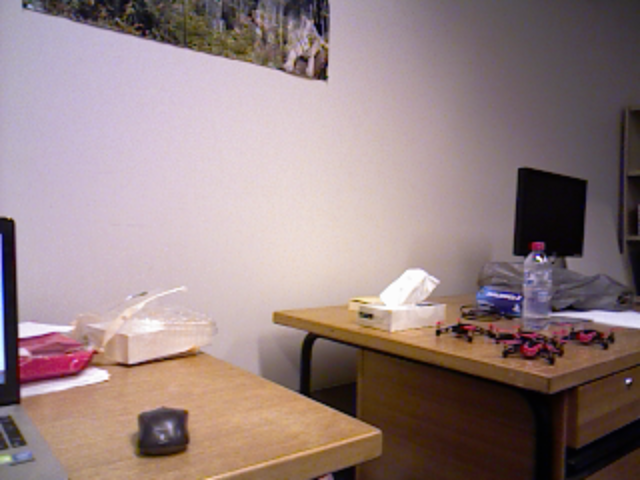
\includegraphics[width=1.7in]{images/ch2/colorF11}
                \caption{Color Image}
                \label{fig:COLEXAMPLE}
        \end{subfigure}%
        \begin{subfigure}[b]{1.8in}
                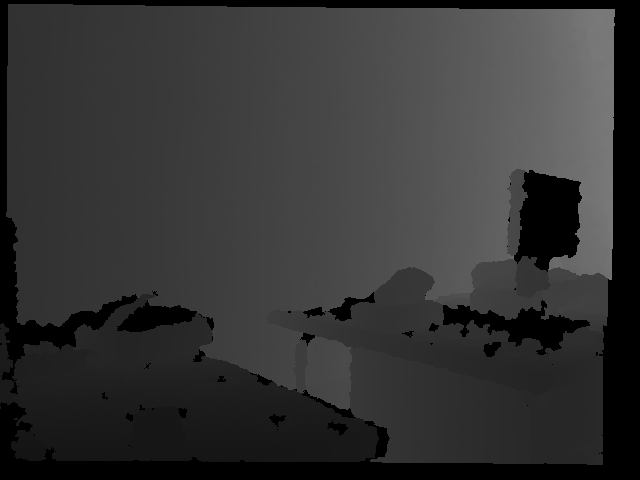
\includegraphics[width=1.7in]{images/ch2/depthF11}
                \caption{Depth Image}
                \label{fig:DEPTHEXAMPLE}
        \end{subfigure}
        
         \begin{subfigure}[b]{1.8in}
                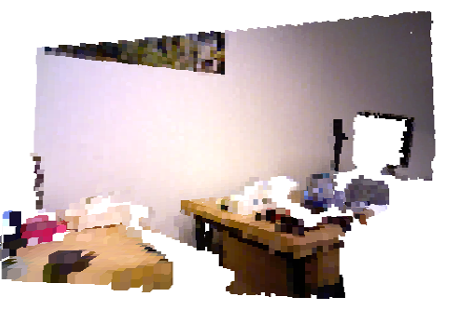
\includegraphics[width=1.8in]{images/ch2/volumeF11128}
                \caption{Projected Volume $128^3$}
                \label{fig:VOLUMEEXAMPLE128}
        \end{subfigure}%
         \begin{subfigure}[b]{1.8in}
                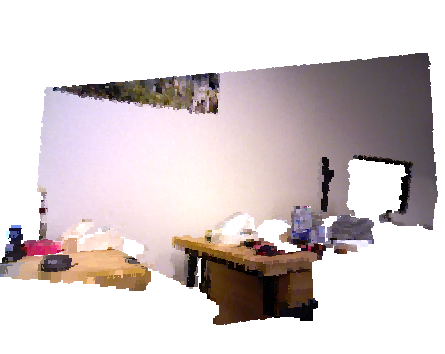
\includegraphics[width=1.8in]{images/ch2/volumeF11256}
                \caption{Projected Volume $256^3$}
                \label{fig:VOLUMEEXAMPLE384}
        \end{subfigure}%
       \caption{A Projected Frame.}
       \label{fig:PROJECTED_FRAME}
\end{figure}


To facilitate further processing, the projected image volumes are re-sampled. The results reported in this paper were obtained using volumes of $256^3$ voxels in size. An example colour and depth image pair and their volumetric projection is shown in figure \ref{fig:PROJECTED_FRAME}.  \\


\subsection{Stereo Camera Based Reconstruction}

The Fourier volume registration methods also work with stereo camera based data. This information can be generated using several of the techniques described in the literature review. Essentially the data must then be projected into depth frames which are registered using one of the proposed fourier volume registration techniques. Because stereo methods do not always accurately compute depth to scale, fourier volume registration has an advantage over other methods in that it also registers against scale. For systems where depth is estimated accurately (as accurately or more than depth sensors) results should work similarly.

\subsection{Monocular Sensor Based 3D Reconstruction}

Some preliminary research has been conducted in evaluating the use of Fourier volume registration given monocular data. From monocular video frames, depth was first computed. This data was fed into the fourier volume registration method in computing 3D reconstructions. Preliminary results are presented but further investigation is required in this area.



\section{Conclusion} % Methodology
\begin{savequote}[8cm]
  ``I just wondered how things were put together.''
  \qauthor{Claude Shannon}
\end{savequote}
\makeatletter
\chapter{Experiments}

\section{Experiments}

\section{Test Data}

Test Data was generated based on the testing requirements for this research. In order to robustly test the different pose-estimation procedures / 3D-registration methods we generated data from a variety of scenes. These scenes include both in-door and out-door scenes, scenes with large amounts of texture and scenes with little to no texture. We also captured scenes which may cause confusion for algorithms which rely on texture information. This data typically has many items which look similar locally but are actually different objects within the scene globally. \\

Moreover, our test-data also measure's each algorithm's ability to register different camera movements by localizing them to different scenes. Different camera motions captured include: camera translation and zooming as well as different axes of rotation. \\

Some frames from the original test-set are shown in appendix \ref{AppendixA}. The first scene: the Apartment Texture Rotate scene was taken by rotating the camera around the y-axis across an apartment. This scene contains plenty of textural information. The Apartment Texture X Axis scene is similar in terms of texture but contains both x and y axis rotation. This tests the Volume Phase Registration algorithm's ability to handle multiple axes of rotation. \\

The boxes scene was captured under arbitrary-rotation, translation and zoom-in/out camera motions. It contains some useful information on the boxes themselves, however the texture on the carpet is of little to no use for most feature based registration methods. The Desk Texture Translation scene contains a desk with a desktop computer and several items on it. The In-door space with texture-confusion contains a set of chairs and picture frames which look similar to eachother locally but may cause confusion for registration techniques which rely on local features.  \\

The kitchen scene was captured with both translation and zoom camera movements. The scene contains very little texture and the color is predominantly white. The Office textured blind-spot rotation scene is a textured office scene where the camera is rotated about the y-axis. The scene is focused on a large divider which seperates two desks. The divider may confuse registration methods which rely too heavily on minimization by aligning the large divider in priority rather than taking into acount the smaller details of the scene. \\

The Office scenes contain a decent amount of usable texture and different sets were created by translating, rotating about the y-axis and rotating about the x-axis. Other office scenes, where the camera has objects in both the foreground and the background and where the camera is lifted and rotated whilst focusing on an office desk/chair. \\

Some out-door scenes were also captured around the university. Scenes are captured with both rotation and translation camera movements. These scenes are also labelled as being susceptable to texture confusion.

\section{Analysis Tools}

In order to test different registration methods. Algorithms were written in C/C++ using both Visual Studio (2012 and 2015) on a Windows (7 \& 10) machine and code-blocks 16 on an Ubuntu machine. All source code is made available online at: https://github.com/lukes611/phdThesis. In order to measure registration algorithms we use the error metrics described in the ERROR METRICS SECTION section.  

\section{Algorithms}

Different 3D-registration algorithms were implemented to test the Fourier Volume Registration (FVR) method. We compared with Feature Matching methods because these methods are still dominant and very successful in image processing and computer vision. In this research we aimed to show that FVR was competitive with these feature matching methods whilst beating them in certain contexts (such as little textuere or scenes where texture confusion may occur). \\ 

We test with both 2D feature matching, where the features are found and matched between a pair of 2D-images, then RANSAC is used with the corresponding matches and true 3D point to compute pose. The pose is then used to reconstruct the scene. We found that SURF performed best out of the other feature matching methods, so we use SURF in our 2D feature matching algorithm. The 2D feature matching method is limited as it cannot register frames which have too few features or frames which contain texture confusion. It is also not able to handle wider base-lines. \\

We also test 3D-feature matching using an implementation of SIFT in 3D. This algorithm was tested and written in C/C++ and is also susceptable to failed registration in scenes with too few features and texture confusion but it shouble be more able to handle wider base-lines than the 2D counterpart as it works in 3D. //

Another algorithm we test against is ICP or Iterative Closest Point. This method has become very popular in 3D reconstruction and works well on most scene types. One disadvantage is that this method may get stuck in a minima and fail to register, this can occur especially when registering wider baselines. \\

The other method we test with is PCA or Principal Components Analysis is actually used to find the mean and principal components of a multi-dimensional data-set. This is useful for registration purposes as it works on wide-baselines, is very fast and provides additional information about a scene. The downside is that is is very susceptable to noisey or mis-aligned data. Our FVR method actually makes use of information from PCA so it is good to compare the two to find out what improvements if any are made by FVR. \\

The final algorithm tested is the proposed FVR algorithm, which uses both PCA and Fourier Phase Correlation to find the registration transformation between two 3D data-sets. This algorithm was proposed to handle general transformations about any rotation axis, translation axis as well as handle scaling. It was also designed to be able to handle noisey data, data with texture-confusion and data with little to no texture making it a viable option in the 3D registration and pose estimation research areas.


\section{Qualitative Experiments}

Our Qualitative experiments were performed by using different algorithms to generate 3D reconstructed scenes. 

\section{Quantitative Experiments}

\subsection{Camera Movement Experiments}

\subsection{Pose Estimation Experiments}

\subsection{Noise Experiments}




\begin{figure*}[t] 
        \centering
        \begin{subfigure}[b]{2.0in}
                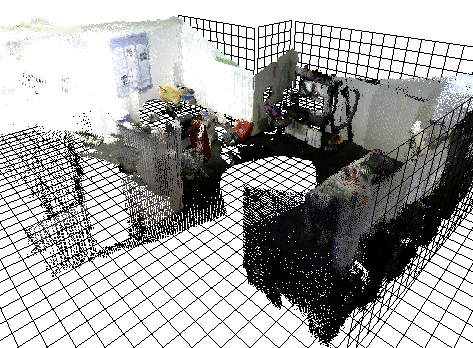
\includegraphics[width=2.0in]{images/ch2/unit21}
                \caption{Apartment}
                \label{fig:RECON_UNIT}
        \end{subfigure}%
        \begin{subfigure}[b]{2.0in}
                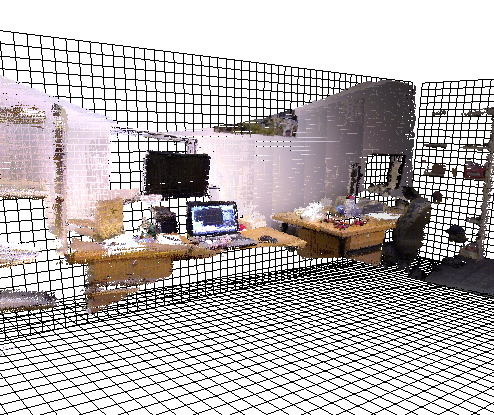
\includegraphics[width=2.0in]{images/ch2/officeA}
                \caption{Office}
                \label{fig:RECON_OFFICE}
        \end{subfigure}%
        \begin{subfigure}[b]{2.0in}
                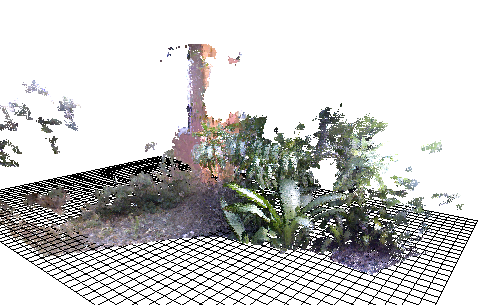
\includegraphics[width=2.0in]{images/ch2/outdoorA}
                \caption{Garden}
                \label{fig:RECON_GARDEN}
        \end{subfigure}
       \caption{Reconstructed Scenes.}
       \label{fig:RECONSTRUCTIONS}
\end{figure*}


\subsection{Codec Evaluation \& Comparison Techniques}

Codec evaluation involves comparing storage requirements between the original model and codec output. In the case of lossy codecs, a quantitative quality metric is also required. Compression metrics are easy to compute, quality metrics are more involved and there have been many proposed techniques. Quality metrics compare the distortion created by the codec relative to the original model. Two measurements are usually performed, the distance from the compressed model to the original and the distance from the original to the compressed model. Quality metrics are split into empirical and perceptual based metrics. Empirical metrics measure geometric error and perceptual metrics estimate human perception. Perception based metrics are a part of psychophysics research. For a more in-depth survey of these methods, see work by Bubill \textit{et al.} \cite{Bulbul11Assessing}.

\subsubsection{Compression Metrics}

In the context of 3D model compression, the file size of both, the compressed model and the original are compared. Alternatively, the file size of the compressed model from one codec can be compared to the file size of the same model compressed using another codec. The compression ratio ($CR$), defined as the original file size divided by the compressed file size, is a measure of compression performance. Another metric used is called the bit rate, different bit rates are used depending on the representation being compressed. The mesh representation uses bits per vertex (bpv) and bits per triangle (bpt), the volumetric representation uses bits per voxel and the point cloud representation uses bits per point.

\subsubsection{Empirical Error Metrics}

The following metrics are used to assess the error between two data samples. For two points, $p$ \& $q$, in $\Re^3$ space, the basic euclidean distance metric,
$$
ED(q,p) = \sqrt{(q_x - p_x)^2 + (q_y - p_y)^2 + (q_z - p_z)^2}
$$,
the absolute error,
$$
AE(q,p) = \|q_x - p_x\| + \|q_y - p_y\| + \|q_z - p_z\|
$$
and the squared error $SE$, 
$$
SE(q,p) = (q_x - p_x)^2 + (q_y - p_y)^2 + (q_z - p_z)^2
$$
are often used as a basis for other metrics. 3D models can be sampled into a set of points in $\Re^3$. Using these samples, the following metrics can be used: sum of distances ($SOD$), sum of absolute differences ($SAD$), sum of squared errors ($SSE$), mean square error ($MSE$) and root mean square error ($RMS$). Since the two models may be sampled differently, the minimum error from one sample to the others is used. These metrics are defined below using two point sets, $A$ \& $B$ where the length of these sets is $M$ and $N$ respectively.
$$
SOD(A,B) = \sum_{k=0}^{M} \min_{b \in B}(ED(A_k,b))
$$

$$
SAD(A,B) = \sum_{k=0}^{M} \min_{b \in B}(AE(A_k,b))
$$

$$
SSE(A,B) = \sum_{k=0}^{M} \min_{b \in B}(SE(A_k,b))
$$

$$
MSE(A,B) = \frac{1}{M}SSE(A,B)
$$

$$
RMS(A,B) = \sqrt{MSE(A,B)}
$$

For each of these metrics, $METRIC(A,B) \neq METRIC(B,A)$. Therefore, these methods are often averaged (below). This is termed the average metric (AM), as opposed to the minimum metric (MM) which is the smallest value of the two.

$$
AvgError = \frac{Metric(A,B)+Metric(B,A)}{2}
$$

Another metric, the Hausdorff distance ($HD$) is a measure of overall shape similarity. It is defined as the largest value of the maximum distances between objects from $A$ to $B$ and from $B$ to $A$. For example, for two objects $A$ \& $B$, the Hausforff distance $HD$, from $A$ to $B$, is defined as,
$$
HD(A,B) = \max(D(A,B),D(B,A))
$$
where $D(A,B)$ is defined as,
$$
D(A,B) = \{a \in A \| \max(dist(a,B)\}
$$
and $dist(a,B)$ is defined below.
$$
dist(a,B) = \{b \in B \left| \min(\|a-b\|)\right.\}
$$

\subsubsection{Human Perception Based Metrics}

Lavoue \textit{et al.} \cite{Lavoue06Perceptually} devised a metric based on structural distortion, this method correlates well with human perception. It is based on the SSIM method of Wang \textit{et al.} \cite{Wang04Image}, which is a popular image metric. Lavoue \textit{et al.} call their method the, Mesh Structural Distortion Measure (MSDM). An updated version of this metric was also developed \cite{Lavoue11Multiscale}.

\paragraph{Laplacian Metric}

Karni \& Gotsman \cite{Karni00Spectral} developed their own on-line metric for use during their spectral based codec. It is based on the laplacian and measures the difference between two objects in terms of their smoothness. 

\paragraph{Elastic Deformation Based Metric}

Bian \textit{et al.} \cite{Bian09Evaluation} developed a novel metric, useful for both on and off-line model comparison. The algorithm is based on the theory of strain fields. A strain field is a metric derived from elasticity, it is used to describe the deformation of some object which has elastic properties. Using this concept, both models are treated as having elastic properties in order to perform quality assessment.

\paragraph{Saliency Based Metrics}

Howlett \textit{et al.} \cite{Howlett04Experimental} and Lee \textit{et al.} \cite{Lee05Mesh} both presented work aimed at determining salient features in 3D models. They incorporated these findings in their own metrics. Howlett \textit{et al.} used a human gaze detection device to study the psychophysical effects of viewing 3D objects. Both of these metrics are based on preserving the sections of the object in which any distortion would be visibly noticeable to humans.

\paragraph{The Depth Difference Metric}

Krivokuca \textit{et al.} \cite{Krivokuca12New} developed a perceptual based metric for the off-line quality assessment of 3D models. This method is independent of model representation and is based on generating multiple depth maps from different orthographic perspectives. It improves upon both the Hausdorff distance and RMS error and is good at detecting both small and large geometric errors. Krivokuca \textit{et al.} call their method, the Depth Difference (DD). It works by comparing orthographic depth maps from both the original and compressed models. First a difference depth image is calculated ($DDI$) from orthographic depth maps of the original object ($DIO$) and of the compressed object ($DIC$). The $DDI$ is calculated using element-wise matrix subtraction,

$$
DDI = DIO - DIC
$$

Then the average depth distance value ($ADD$) is calculated from the $DDI$ matrix, this equation is presented below.

$$
ADD = \frac{1}{MN} \sum_{y=0}^{M} \sum_{x=0}^{N} DDI_{y,x}
$$

This $ADD$ value is then summed up and averaged over different orthographic views, this average is the Depth Difference.

 % Experiments &
\section{Results}

%in methodology section?
\section{Test Data}

\section{Analysis Tools}

\section{Qualitative Experiments}

\section{Quantitative Experiments}

\subsection{Pose Estimation Experiments}

\begin{figure*}[t!] 
        \centering
        \begin{subfigure}[b]{6.0in}
                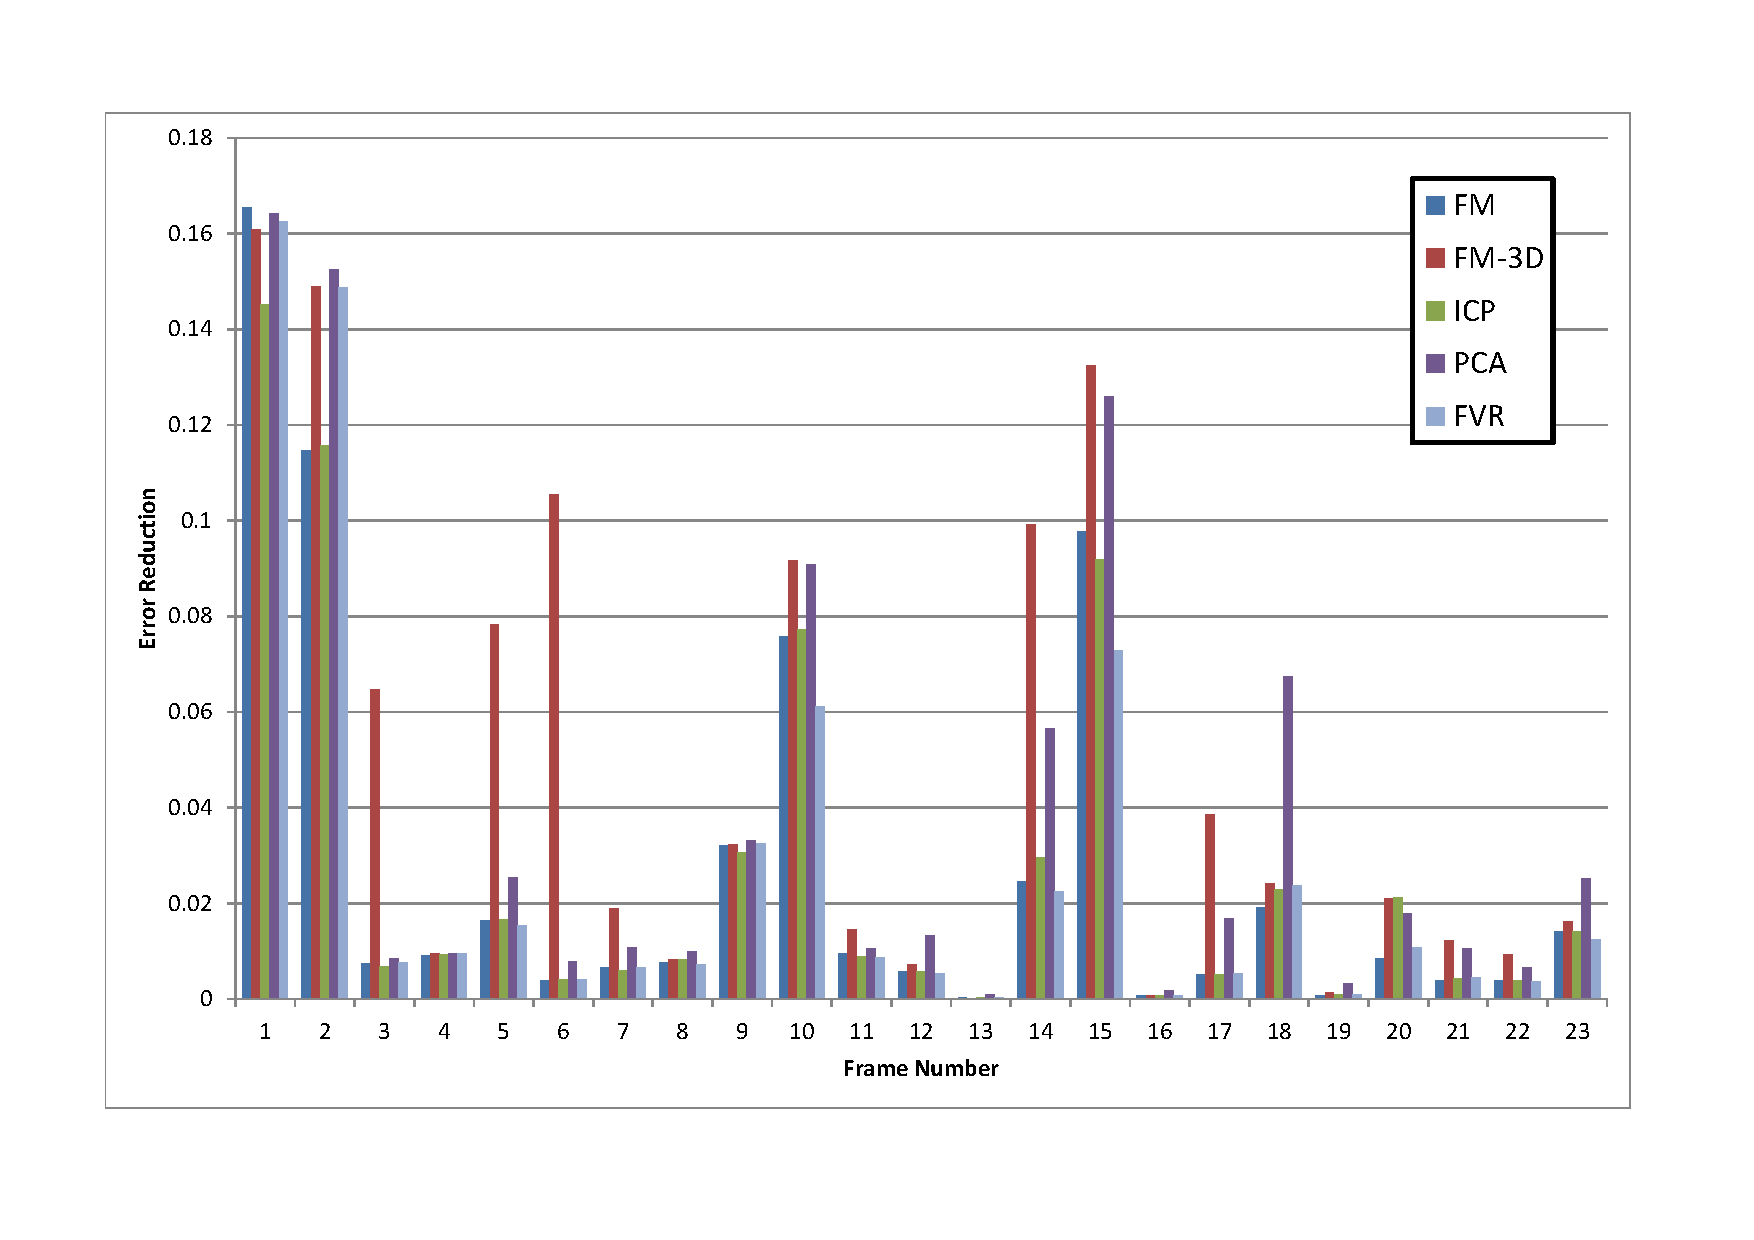
\includegraphics[width=6.0in]{images/results/Apartment_Texture_Rotate}
                \caption{original}
                \label{fig:PEE1}
        \end{subfigure}
       \caption{Registration improvements for Apartment Texture Rotate for different methods.}\label{fig:PEE1Fig}
\end{figure*}

\begin{figure*}[t!] 
        \centering
        \begin{subfigure}[b]{6.0in}
                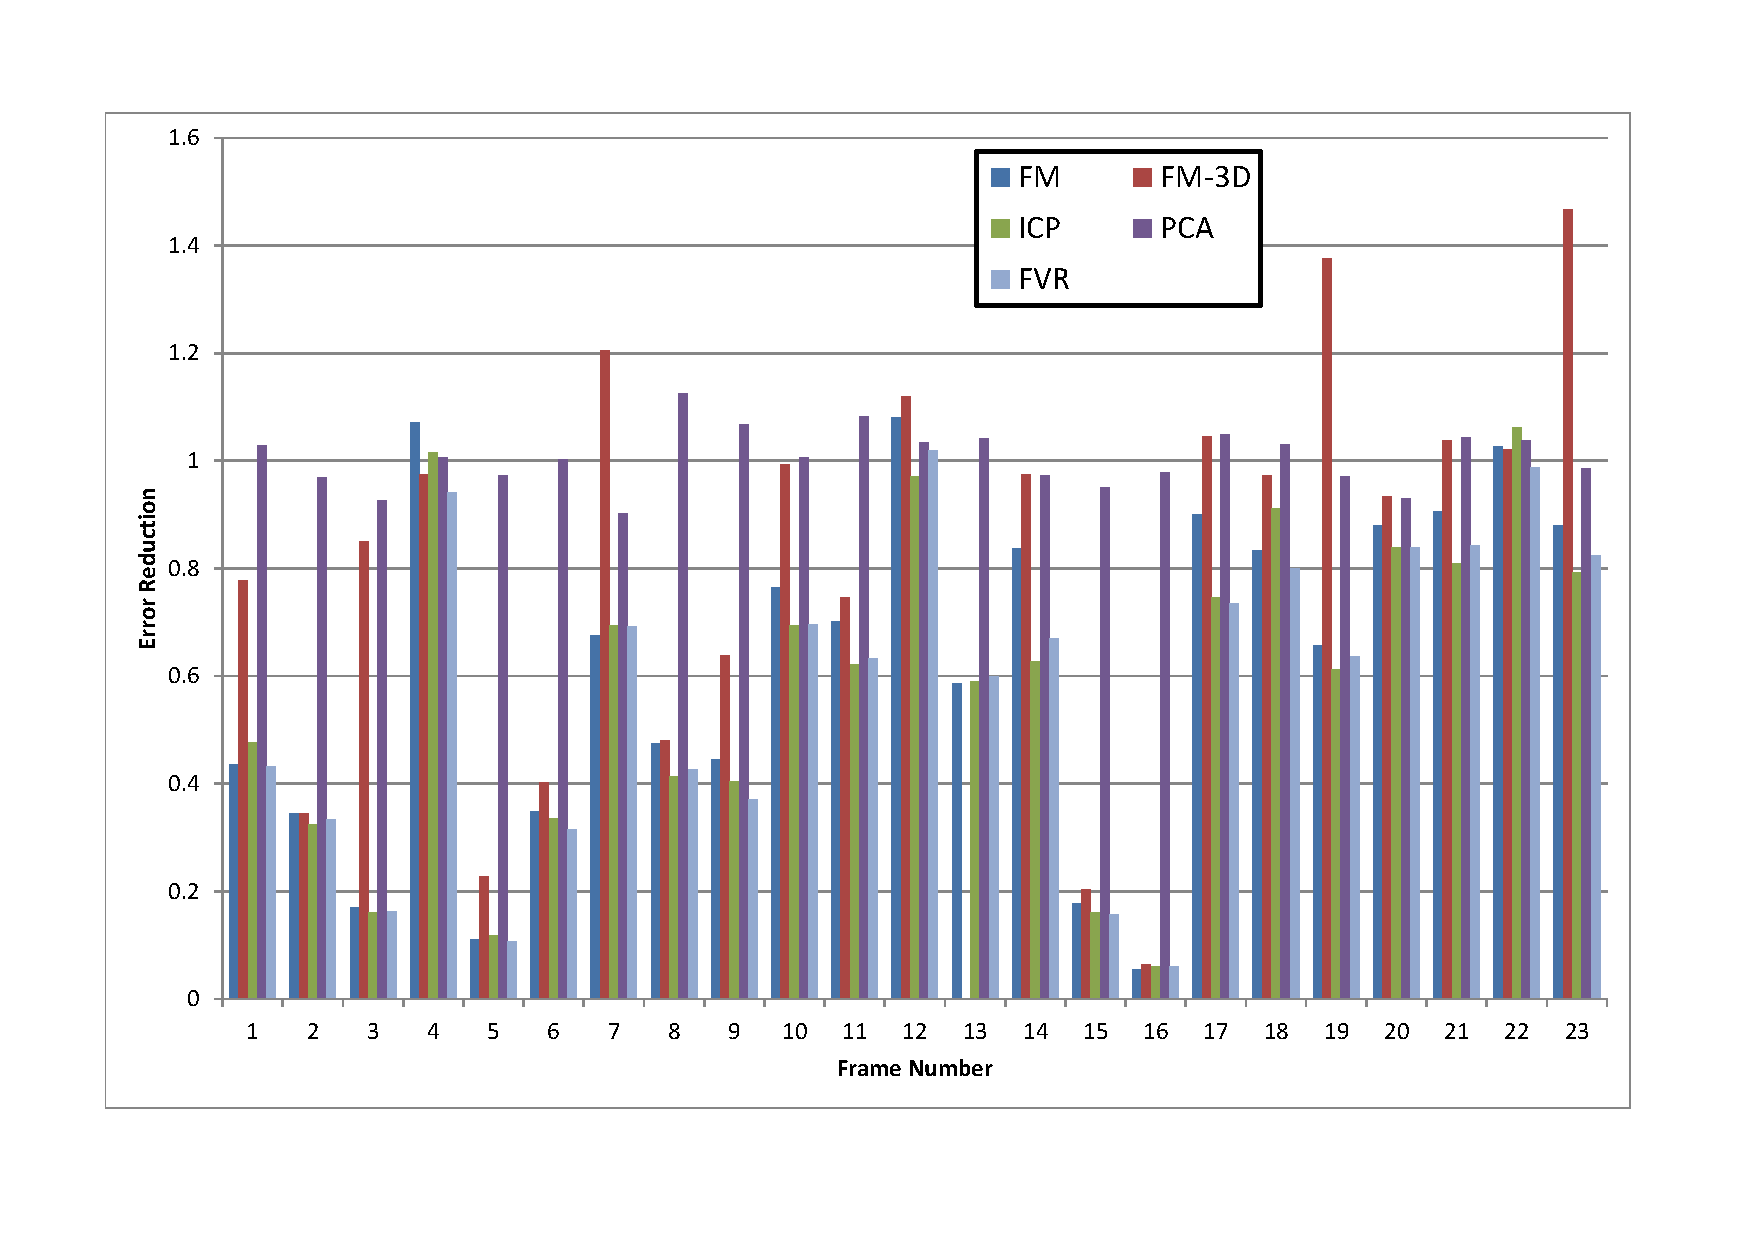
\includegraphics[width=6.0in]{images/results/Apartment_Texture_Rotate_XAxis}
                \caption{original}
                \label{fig:PEE2}
        \end{subfigure}
       \caption{Registration improvements for Apartment Texture X-Axis Rotate for different methods.}\label{fig:PEE2Fig}
\end{figure*}


\begin{figure*}[t!] 
        \centering
        \begin{subfigure}[b]{6.0in}
                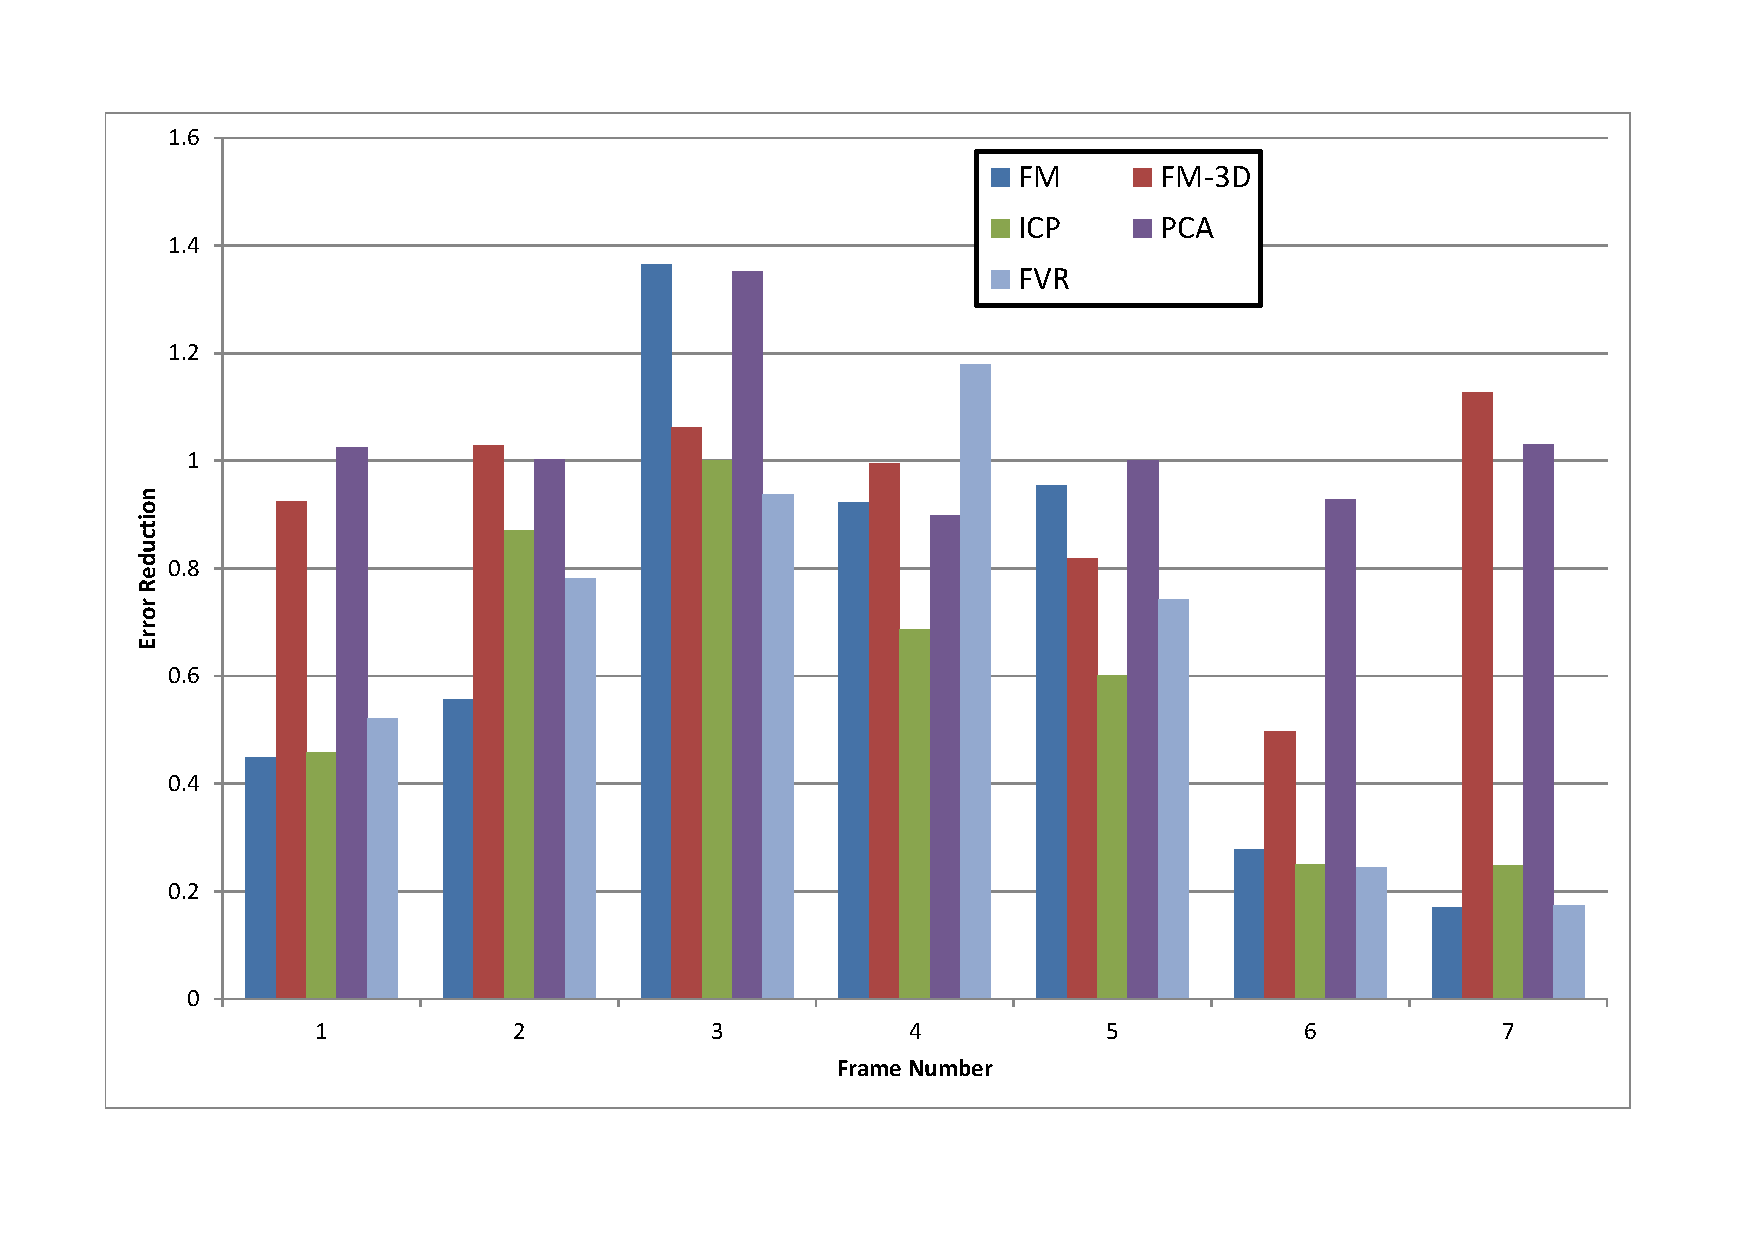
\includegraphics[width=6.0in]{images/results/Boxes_Texture_Rotate}
                \caption{original}
                \label{fig:PEE3}
        \end{subfigure}
       \caption{Registration improvements for Boxes Texture Rotate for different methods.}\label{fig:PEE3Fig}
\end{figure*}

\subsection{3D Registration Experiments}

\subsection{Noise Robustness Tests}

hi


\section{Conclusion}
 % Results
\begin{savequote}[8cm]
  ``Learn from yesterday, live for today, hope for tomorrow. The important thing is not to stop questioning.''
  \qauthor{Albert Einstein}
\end{savequote}
\makeatletter
\chapter{Conclusion}

\section{Research Aims Revisited}

The primary aim of this research was to improve the storage, quantitative quality and perceptual quality of 3D models. Hierarchical methods were investigated and this led to a new image codec, ILQT \cite{Lincoln13Interpolating} as well as the proposed scheme, the Shade-Octree. The research question was, ``Do hierarchical techniques bring state of the art compression performance to 3D data?'' Results from chapter 4 show that the SOT outperforms the OT compression scheme as well as several state of the art methods in terms of rate-distortion and perceptual quality. The primary aim of this research has been accomplished because the SOT produces models which have improved storage efficiency, whilst improving quantitative quality and perceptual quality compared with other compression schemes. The proposed research question can also be answered. The SOT, a hierarchical codec, does achieve state of the art performance in the field of 3D data compression.

\section{Future Work}

There is still much work to be done in the area of hierarchical 3D data compression. One possible project could be to improve the SOT. Currently the SOT can produce holes in the output mesh, an investigation of this may lead to improved results. Other projects could investigate the extension of the PJQ, wedglet, BSP-tree and QB tree to 3D model compression.
 % Conclusion
\appendix
none
\makeatletter
\chapter{Appendix A}
\label{AppendixA}

\section{Test Data}

%keep
\begin{figure*}[t]
\centering
\begin{subfigure}[b]{1.5in}
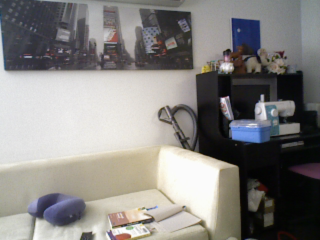
\includegraphics[width=1.5in]{{images/experiments/test_data/Apartment.Texture.rotate.0}.png}
\caption{Frame 1}
\end{subfigure}%
\begin{subfigure}[b]{1.5in}
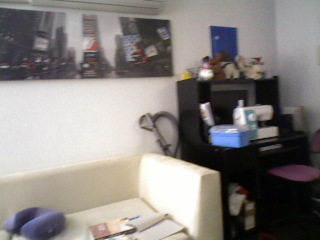
\includegraphics[width=1.5in]{{images/experiments/test_data/Apartment.Texture.rotate.1}.png}
\caption{Frame 10}
\end{subfigure}%
\begin{subfigure}[b]{1.5in}
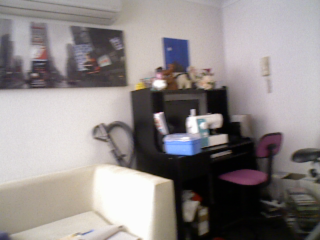
\includegraphics[width=1.5in]{{images/experiments/test_data/Apartment.Texture.rotate.2}.png}
\caption{Frame 15}
\end{subfigure}%
\begin{subfigure}[b]{1.5in}
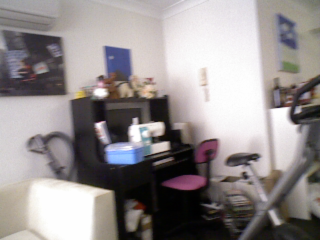
\includegraphics[width=1.5in]{{images/experiments/test_data/Apartment.Texture.rotate.3}.png}
\caption{Frame 20}
\end{subfigure}%
\caption{Four Sample Frames from the Apartment Texture Rotate Data Set}
\label{fig:Apartment_Texture_rotate}
\end{figure*}


%keep
\begin{figure*}[t]
\centering
\begin{subfigure}[b]{1.5in}
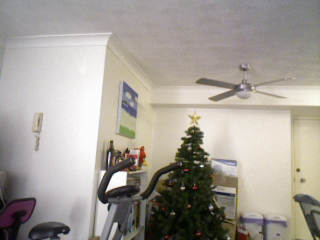
\includegraphics[width=1.5in]{{images/experiments/test_data/Apartment.Texture.rotateXAxis.0}.png}
\caption{Frame 1}
\end{subfigure}%
\begin{subfigure}[b]{1.5in}
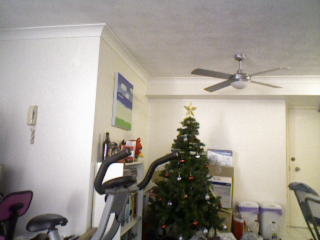
\includegraphics[width=1.5in]{{images/experiments/test_data/Apartment.Texture.rotateXAxis.1}.png}
\caption{Frame 10}
\end{subfigure}%
\begin{subfigure}[b]{1.5in}
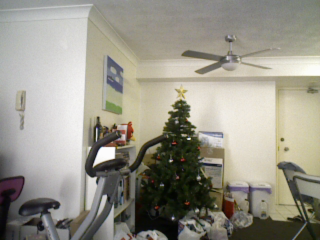
\includegraphics[width=1.5in]{{images/experiments/test_data/Apartment.Texture.rotateXAxis.2}.png}
\caption{Frame 15}
\end{subfigure}%
\begin{subfigure}[b]{1.5in}
\includegraphics[width=1.5in]{{images/experiments/test_data/Apartment.Texture.rotateXAxis.3}.png}
\caption{Frame 20}
\end{subfigure}%
\caption{Four Sample Frames from the Apartment Texture X-Axis Rotation Data Set.}
\label{fig:Apartment_Texture_rotateXAxis}
\end{figure*}


%keep
\begin{figure*}[t]
\centering
\begin{subfigure}[b]{1.5in}
\includegraphics[width=1.5in]{{images/experiments/test_data/Desk.Texture.Translation.0}.png}
\caption{Frame 1}
\end{subfigure}%
\begin{subfigure}[b]{1.5in}
\includegraphics[width=1.5in]{{images/experiments/test_data/Desk.Texture.Translation.1}.png}
\caption{Frame 10}
\end{subfigure}%
\begin{subfigure}[b]{1.5in}
\includegraphics[width=1.5in]{{images/experiments/test_data/Desk.Texture.Translation.2}.png}
\caption{Frame 15}
\end{subfigure}%
\begin{subfigure}[b]{1.5in}
\includegraphics[width=1.5in]{{images/experiments/test_data/Desk.Texture.Translation.3}.png}
\caption{Frame 20}
\end{subfigure}%
\caption{Four Sample Frames from the Desk Texture Translation Data Set.}
\label{fig:Desk_Texture_Translation}
\end{figure*}


%keep
\begin{figure*}[t]
\centering
\begin{subfigure}[b]{1.5in}
\includegraphics[width=1.5in]{{images/experiments/test_data/Office.Texture.blindSpotRotation.0}.png}
\caption{Frame 1}
\end{subfigure}%
\begin{subfigure}[b]{1.5in}
\includegraphics[width=1.5in]{{images/experiments/test_data/Office.Texture.blindSpotRotation.1}.png}
\caption{Frame 10}
\end{subfigure}%
\begin{subfigure}[b]{1.5in}
\includegraphics[width=1.5in]{{images/experiments/test_data/Office.Texture.blindSpotRotation.2}.png}
\caption{Frame 15}
\end{subfigure}%
\begin{subfigure}[b]{1.5in}
\includegraphics[width=1.5in]{{images/experiments/test_data/Office.Texture.blindSpotRotation.3}.png}
\caption{Frame 20}
\end{subfigure}%
\caption{Four Sample Frames from the Office Texture.blind-spot Rotation Data Set.}
\label{fig:Office_Texture_blindSpotRotation}
\end{figure*}


%keep
\begin{figure*}[t]
\centering
\begin{subfigure}[b]{1.5in}
\includegraphics[width=1.5in]{{images/experiments/test_data/Office.TexturedItems.Translation.0}.png}
\caption{Frame 1}
\end{subfigure}%
\begin{subfigure}[b]{1.5in}
\includegraphics[width=1.5in]{{images/experiments/test_data/Office.TexturedItems.Translation.1}.png}
\caption{Frame 10}
\end{subfigure}%
\begin{subfigure}[b]{1.5in}
\includegraphics[width=1.5in]{{images/experiments/test_data/Office.TexturedItems.Translation.2}.png}
\caption{Frame 15}
\end{subfigure}%
\begin{subfigure}[b]{1.5in}
\includegraphics[width=1.5in]{{images/experiments/test_data/Office.TexturedItems.Translation.3}.png}
\caption{Frame 20}
\end{subfigure}%
\caption{Four Sample Frames from the Office Textured Items Translation Data Set.}
\label{fig:Office_TexturedItems_Translation}
\end{figure*}


%keep
\begin{figure*}[t]
\centering
\begin{subfigure}[b]{1.5in}
\includegraphics[width=1.5in]{{images/experiments/test_data/Office.Texture.rotation.0}.png}
\caption{Frame 1}
\end{subfigure}%
\begin{subfigure}[b]{1.5in}
\includegraphics[width=1.5in]{{images/experiments/test_data/Office.Texture.rotation.1}.png}
\caption{Frame 10}
\end{subfigure}%
\begin{subfigure}[b]{1.5in}
\includegraphics[width=1.5in]{{images/experiments/test_data/Office.Texture.rotation.2}.png}
\caption{Frame 15}
\end{subfigure}%
\begin{subfigure}[b]{1.5in}
\includegraphics[width=1.5in]{{images/experiments/test_data/Office.Texture.rotation.3}.png}
\caption{Frame 20}
\end{subfigure}%
\caption{Four Sample Frames from the Office Texture Rotation Data Set.}
\label{fig:Office_Texture_rotation}
\end{figure*}



\chapter{Appendix B}
\label{RawQuantitative1}

\section{Registration Errors}

\chapter{Appendix C}
\label{RawQuantitative2}

\section{Noise Results} % Appendix A
\backmatter
\openup -0.5em
%\bibliographystyle{plain}
\bibliographystyle{IEEEtran}
\bibliography{bibliographies/slam,bibliographies/compress}
\end{document}